The content you've provided is LaTeX code, which is a typesetting system used for creating documents. The code you've provided doesn't contain any text that needs to be translated into English. It's mostly defining styles, colors, and new commands. 

For example, the command `\definecolor{mGreen}{rgb}{0,0.5,0}` is defining a new color named `mGreen` with the RGB values of 0, 0.5, 0. 

The command `\newcommand{\sys}{{\textsc{SocksDirect}}\xspace}` is defining a new command named `\sys` that will output the text "SocksDirect" in small caps.

The command `\newenvironment{icompact}` is defining a new environment for lists with specific parameters for parsep, partopsep, topsep, itemsep, parskip, and leftmargin.

If you have any text content in your LaTeX document that needs to be translated into English, please provide that.

\chapter{Acceleration of SocksDirect Communication Primitives}
\label{chapter:socksdirect}

% !TeX root = ../main.tex
\chapter{绪论}

\section{研究的背景和意义}

随着互联网的发展,互联网数据中心(Internet Data Center,IDC)在世界各地兴起。21 世纪第一个十年,数据中心主要处理 Web 网站、搜索引擎等容易并行的任务。因此,互联网数据中心多使用大量低成本的标准服务器搭建。

近十年来,大数据处理与机器学习的兴起改变了数据中心的负载特性。一方面,大数据处理、机器学习等负载对算力要求很高。与此同时,由于 Dennard 缩放定律的终结,近十年来,通用处理器的频率提升和多核核数增加都受到功耗墙的限制。因此,通用处理器性能提升 ``免费的午餐'' 已经结束,体系结构的创新迎来了春天,GPU、FPGA、TPU 等定制化硬件在数据中心内大量部署。另一方面,大数据处理、机器学习等负载需要多个节点紧密协同处理,对节点间的通信带宽和延迟要求较高。因此,近十年来,数据中心网络从 1 Gbps 发展到 40 Gbps,并有向 100 Gbps 演进的趋势。定制化硬件之间的专用互连也成为趋势。

与此同时,数据中心的运营模式也在经历一场云化的变革。数据中心的算力逐渐集中到少数几家云厂商,每家拥有数以百万计的服务器。

因此,如英伟达 CEO 黄仁勋所说,未来的数据中心会像超级计算机一样。




\begin{figure}[htbp]
	\centering
	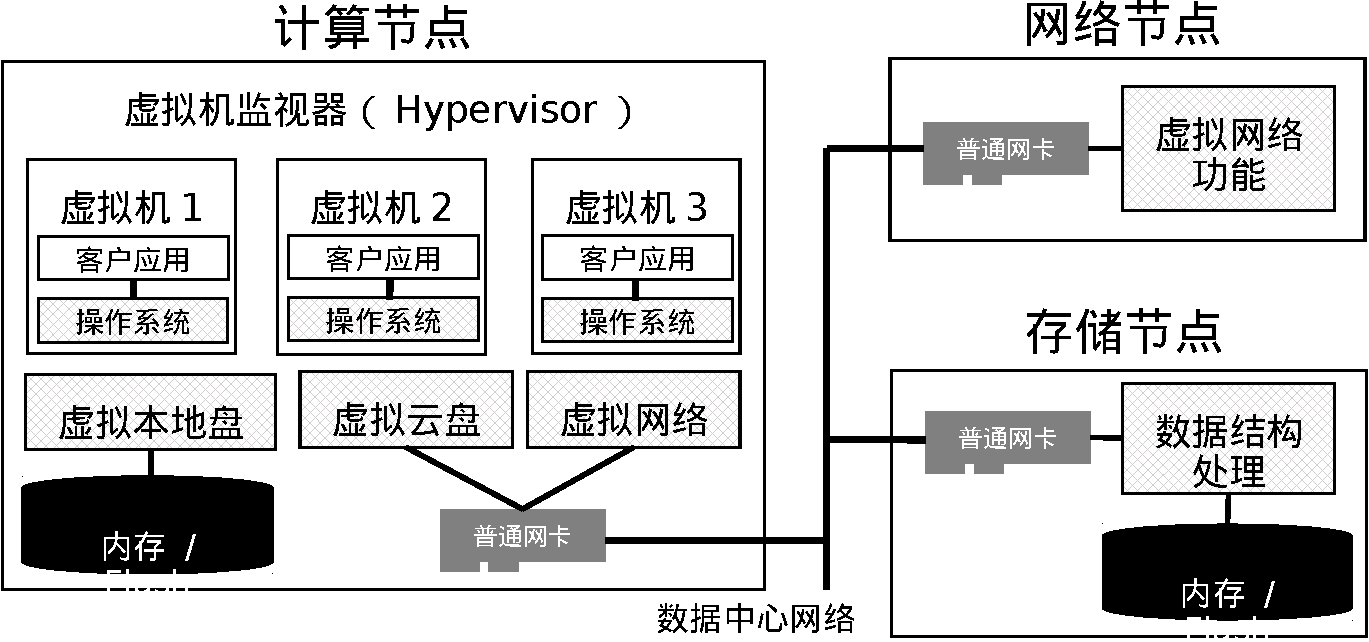
\includegraphics[width=0.8\textwidth]{figures/virt_arch.pdf}
	\caption{虚拟化的数据中心架构。}
	\label{background:fig:virt-architecture}
\end{figure}

\section{国内外研究现状}




第二章提炼 2 页

\section{本文的研究内容和贡献}



\begin{figure}[htbp]
	\centering
	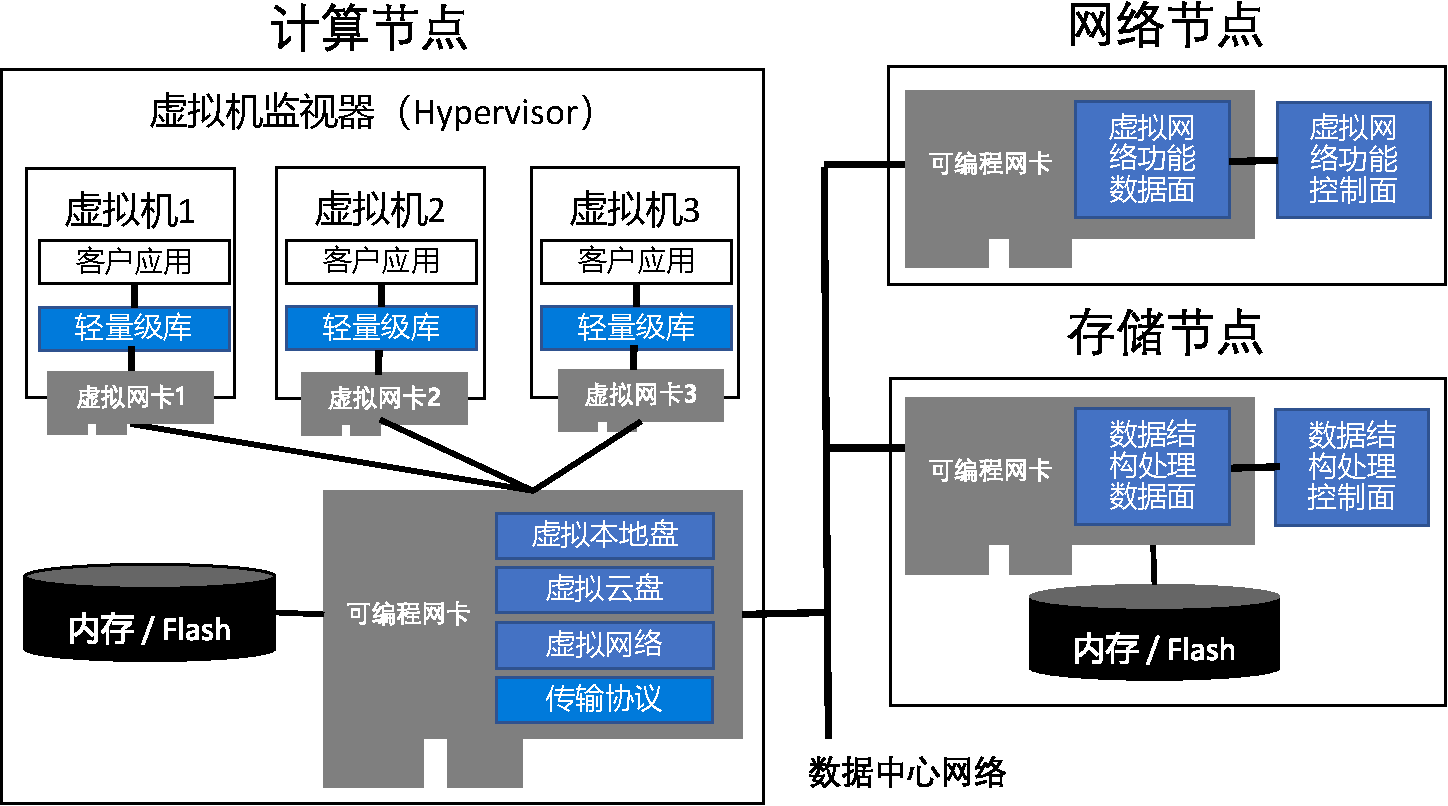
\includegraphics[width=0.8\textwidth]{figures/accel_arch.pdf}
	\caption{基于可编程网卡的数据中心系统总体架构。}
	\label{arch:fig:accel-arch}
\end{figure}

摘要的扩充,第三章提炼 2 页

\section{论文结构安排}

本论⽂的内容结构安排如下:
第 1 章为绪论。
第 2 章介绍了数据中心的背景知识和硬件的发展趋势,分析了可编程网卡的四种架构,并调研了可编程网卡在数据中心的应用。
第 3 章提出了基于可编程网卡的高性能数据中心系统架构。
第 4 章提出用可编程网卡加速云计算中的虚拟网络功能。为了简化FPGA编程,提出了首个适用于高速网络数据包处理、基于高级语言的模块化FPGA编程框架ClickNP。
第 5 章提出用可编程网卡加速远程数据结构访问,并设计实现了一个高性能内存键值存储系统 KV-Direct。
第 6 章提出用可编程网卡和用户态运行库相结合的方法为应用程序提供系统原语,并设计实现了一个用户态套接字系统 SocksDirect。
第 7 章总结全⽂并展望未来研究方向。
%!TEX root=main.tex
\chapter{数据中心与可编程网卡概论}
\label{chapter:background}

本章介绍全文的背景和相关工作。第 1 节回顾数据中心的发展历史,展望数据中心的未来趋势,提出数据中心的性能开销与挑战,以及性能优化的可能方向。第 2 节综述数据中心计算、内存、存储和网络互连系统硬件的发展趋势。第 3 节讨论基于专用芯片、网络处理器、通用处理器、FPGA 的四种可编程网卡架构。第 4 节调研可编程网卡在微软 Azure、亚马逊 AWS 等数据中心的部署。

\section{数据中心的性能挑战}
\label{background:sec:challenge}

\subsection{数据中心的过去、现在与未来}

从 20 世纪 50 年代计算机的诞生到 90 年代互联网兴起前,人类的算力大部分用于高性能计算、数字化企业和个人计算机(PC),其产生的数据大多存储在一个个信息孤岛上。需要处理大量信息的大型机乃至超级计算机一般采用软硬件一体化系统,即软硬件是由同一个公司团队开发的。由于采用了高速硬件互连、硬件冗余,这些系统往往同时具备高性能和高可靠性,但成本随系统规模的扩大急剧增加。为了充分利用昂贵的计算机,虚拟化的概念应运而生。其中 20 世纪 50 至 60 年代的分时系统 \cite{strachey1959time,amdahl1964architecture} 实现了多个用户任务分时复用硬件,发展成为 70 年代 UNIX 等现代操作系统 \cite{bach1986design} 的前身。20 世纪 70 至 90 年代,虚拟机监视器(Virtual Machine Monitor,VMM)进一步实现了多个操作系统分时复用硬件 \cite{popek1974formal,agesen2010evolution},为云计算的发展做了技术准备。

20 世纪末,连接信息孤岛的搜索引擎拉开了互联网时代的序幕。数据中心不仅需要搜集、处理和索引海量信息,还需要实时响应大量用户的信息检索请求。传统的超级计算机、大型机和企业级存储不仅成本高昂,也无法满足海量信息存储和用户请求处理的可扩放性。为此,Google 提出用普通商用服务器组建可扩放的数据中心,用软件来实现存储的分区和冗余、用户请求的分派,在相对不可靠的硬件基础上组建起容错的系统 \cite{dean2008mapreduce}。

这些普通商用服务器之所以成本较低,是因为它的架构与大量商用的个人计算机(PC)类似,CPU、内存、主板、硬盘、网卡等组成部分都是标准组件,由各个专业公司独立设计实现。操作系统、数据库、Web 服务器等软件也是标准化的,或者由专业公司开发,或者是开源软件。产量大的标准组件能更好地平摊研发、流片等一次性工程费用(Non-Recurring Engineering,NRE),从而降低标准组件的价格。由标准组件构成的系统虽然降低了数据中心的软硬件成本,但也给标准组件的开发者施加了限制:大家需要遵守标准组件之间的接口和协议,只能在自己的边界内创新。数据中心系统的搭建者则只能像搭积木一样组合标准组件,而很难通盘考虑、全局优化。

21 世纪的第一个十年,互联网的发展让越来越多的企业需要提供 24 小时运行的网络服务,互联网数据中心(Internet Data Center,IDC)托管服务逐渐兴起。然而,IDC 托管需要客户事先购买服务器硬件,并需要运维人员维护,有较高的资产成本(capex)和运营成本(opex)。很多企业的网络服务一方面具有较高的季节性(如亚马逊的黑五促销),因此在闲时大量的计算资源被闲置;另一方面数据和用户规模的扩张很快,给购买硬件和 IDC 选址带来了时间压力。为此,虚拟机托管服务提供了按需租用的虚拟机资源,实现了服务器资源按 CPU 核的切片和在不同客户间的分时复用,也便于客户内部运维人员的管理和调度。

云计算是虚拟机托管服务的升级版,标志性的变革是计算和存储的解耦。虚拟主机托管服务把一台主机上的计算和存储资源分片成多个虚拟机,一旦主机的硬件或虚拟化软件(hypervisor)发生故障,虚拟机也就停机,其中的数据还有丢失的风险。在云计算中,虚拟机的存储资源在分布式存储系统中有多个副本,从而计算节点发生故障时可以从其他计算节点重启虚拟机,存储节点的故障则一般对客户透明。计算和存储的解耦不仅大大提高了服务可用性和数据安全性,也方便了虚拟化软件升级和虚拟机热迁移。


\textbf{云的趋势。摩尔定律。}

\textbf{10 年前,大规模数据处理。}

\textbf{5 年前,深度学习开始兴起。}

\iffalse

\textbf{产品容易传输、各行各业都能用到的基础设施会云化……}
电力作为工业和城市的基础资源,早期也是由需要电的工厂、学校等自己购买发电机来发电,逐渐才形成今天庞大而复杂的电力系统,由发电、输电、变电、配售电等多个标准化的环节构成,客户只需要按需租用电力资源。
计算机作为信息社会的基础设施,自然也不例外。从早期的客户自己购买和运维计算机、操作系统、应用程序,到今天被称为云计算的按需租用计算、存储和网络资源甚至更上层的应用服务。
未来,对提供互联网服务的公司和个人而言,自建数据中心、购买和运维服务器就像自建发电厂、购买和维护发电机一样,在大多数场景下成本很高且没有必要。

随着云计算的发展,工程师们重新获得了在计算机全栈(full-stack)上创新的机会。在云计算平台中,软件和硬件的环境都由服务商控制,在达到了一定的规模以后,各种形式的定制(customization)都成为可能。只要能够提高性能,降低价格,增强竞争力,云服务商有足够的动力去定制芯片,改变网络协议,改变服务器架构,更改操作系统,甚至重新编写应用程序。下一代云平台想要保持竞争优势,除了完善的软件栈外,还必须在体系结构上创新。像过去一样完全使用现成部件(off-the-shelf components)就可以构建有竞争力的公有云平台的时代已经一去不复返了。而在不远的未来,这些云端体系结构的创新必然会向下流动,对未来私有云、企业服务器甚至个人计算机和移动计算的体系结构都会带来深远影响。
\fi

\textbf{云计算和 5G 需要虚拟化,需要灵活性、可编程性和可调试性}


\textbf{计算粒度:从物理机,到虚拟机,到容器(基于容器的微服务),到函数 Granular Computing}

例如,微信有超过 3000 个微服务运行在超过 2 万台服务器上。入口层的微服务每天响应 100 亿至 1000 亿次用户请求,而每个用户请求会在系统内部触发更多的微服务请求,因此整个微信后端每秒需要响应数以亿计的微服务请求 \cite{zhou2018overload}。

加州大学伯克利分校对无服务器计算(serverless computing)的预测报告 \cite{jonas2019cloud} 表明,尽管无服务器计算的范式有诸多优势,也是各大云服务商争相推广的新服务,但由于云存储的性能问题和临时存储服务的缺失,很多类型的应用使用无服务器计算的性能和成本不理想。


\subsection{虚拟化的数据中心架构}

中国系统科学的先驱钱学森老先生说: ``任何事物的开始总是比较简陋的,只有在不断发展的过程中才逐渐完善,逐渐形成一整套复杂而又有机地结合着的体系。'' \cite{qianxuesen}
例如,火车和飞机作为交通工具,早期没有火车站、机场,没有车辆段、修配厂等辅助设施,更没有铁路行车信号、空中交通管制和相关的法律法规。
云计算的发展也是相似的。
使用 OpenStack 开源软件中的一部分组件,我们就可以轻松地搭建出一个由管理、计算、存储节点构成的私有云,满足实验室或小型公司内部的搭建 Web 服务、共享文件、OA 系统等需求。
然而,如果是针对学校或中型公司的需求,就需要支持不同部门之间的隔离……需要 VPC 的概念,网络虚拟化,网络节点承载网络功能……
如果需要大数据处理,深度学习,需要不同硬件,高性能互连……还需要共享数据结构存储……
发展到现代的公有云,提供了上百种不同层次的服务和解决方案。
\textbf{补全}

尽管现代的云计算平台服务多样、结构复杂,其基础也是计算机所必需的计算、内存、存储、网络和互连资源。
在目前基于机架服务器的数据中心中,由于计算设备和内存间高带宽、低延迟的需求,计算和内存一般是绑定在同一台服务器中的。
为了高效地共享计算、存储和网络互连资源,这些资源都被虚拟化,由池化的机架服务器节点提供。
庞大而又复杂的云服务体系是由计算节点池、网络节点池、存储节点池和管理节点池构成的。

\begin{figure}[htbp]
	\centering
	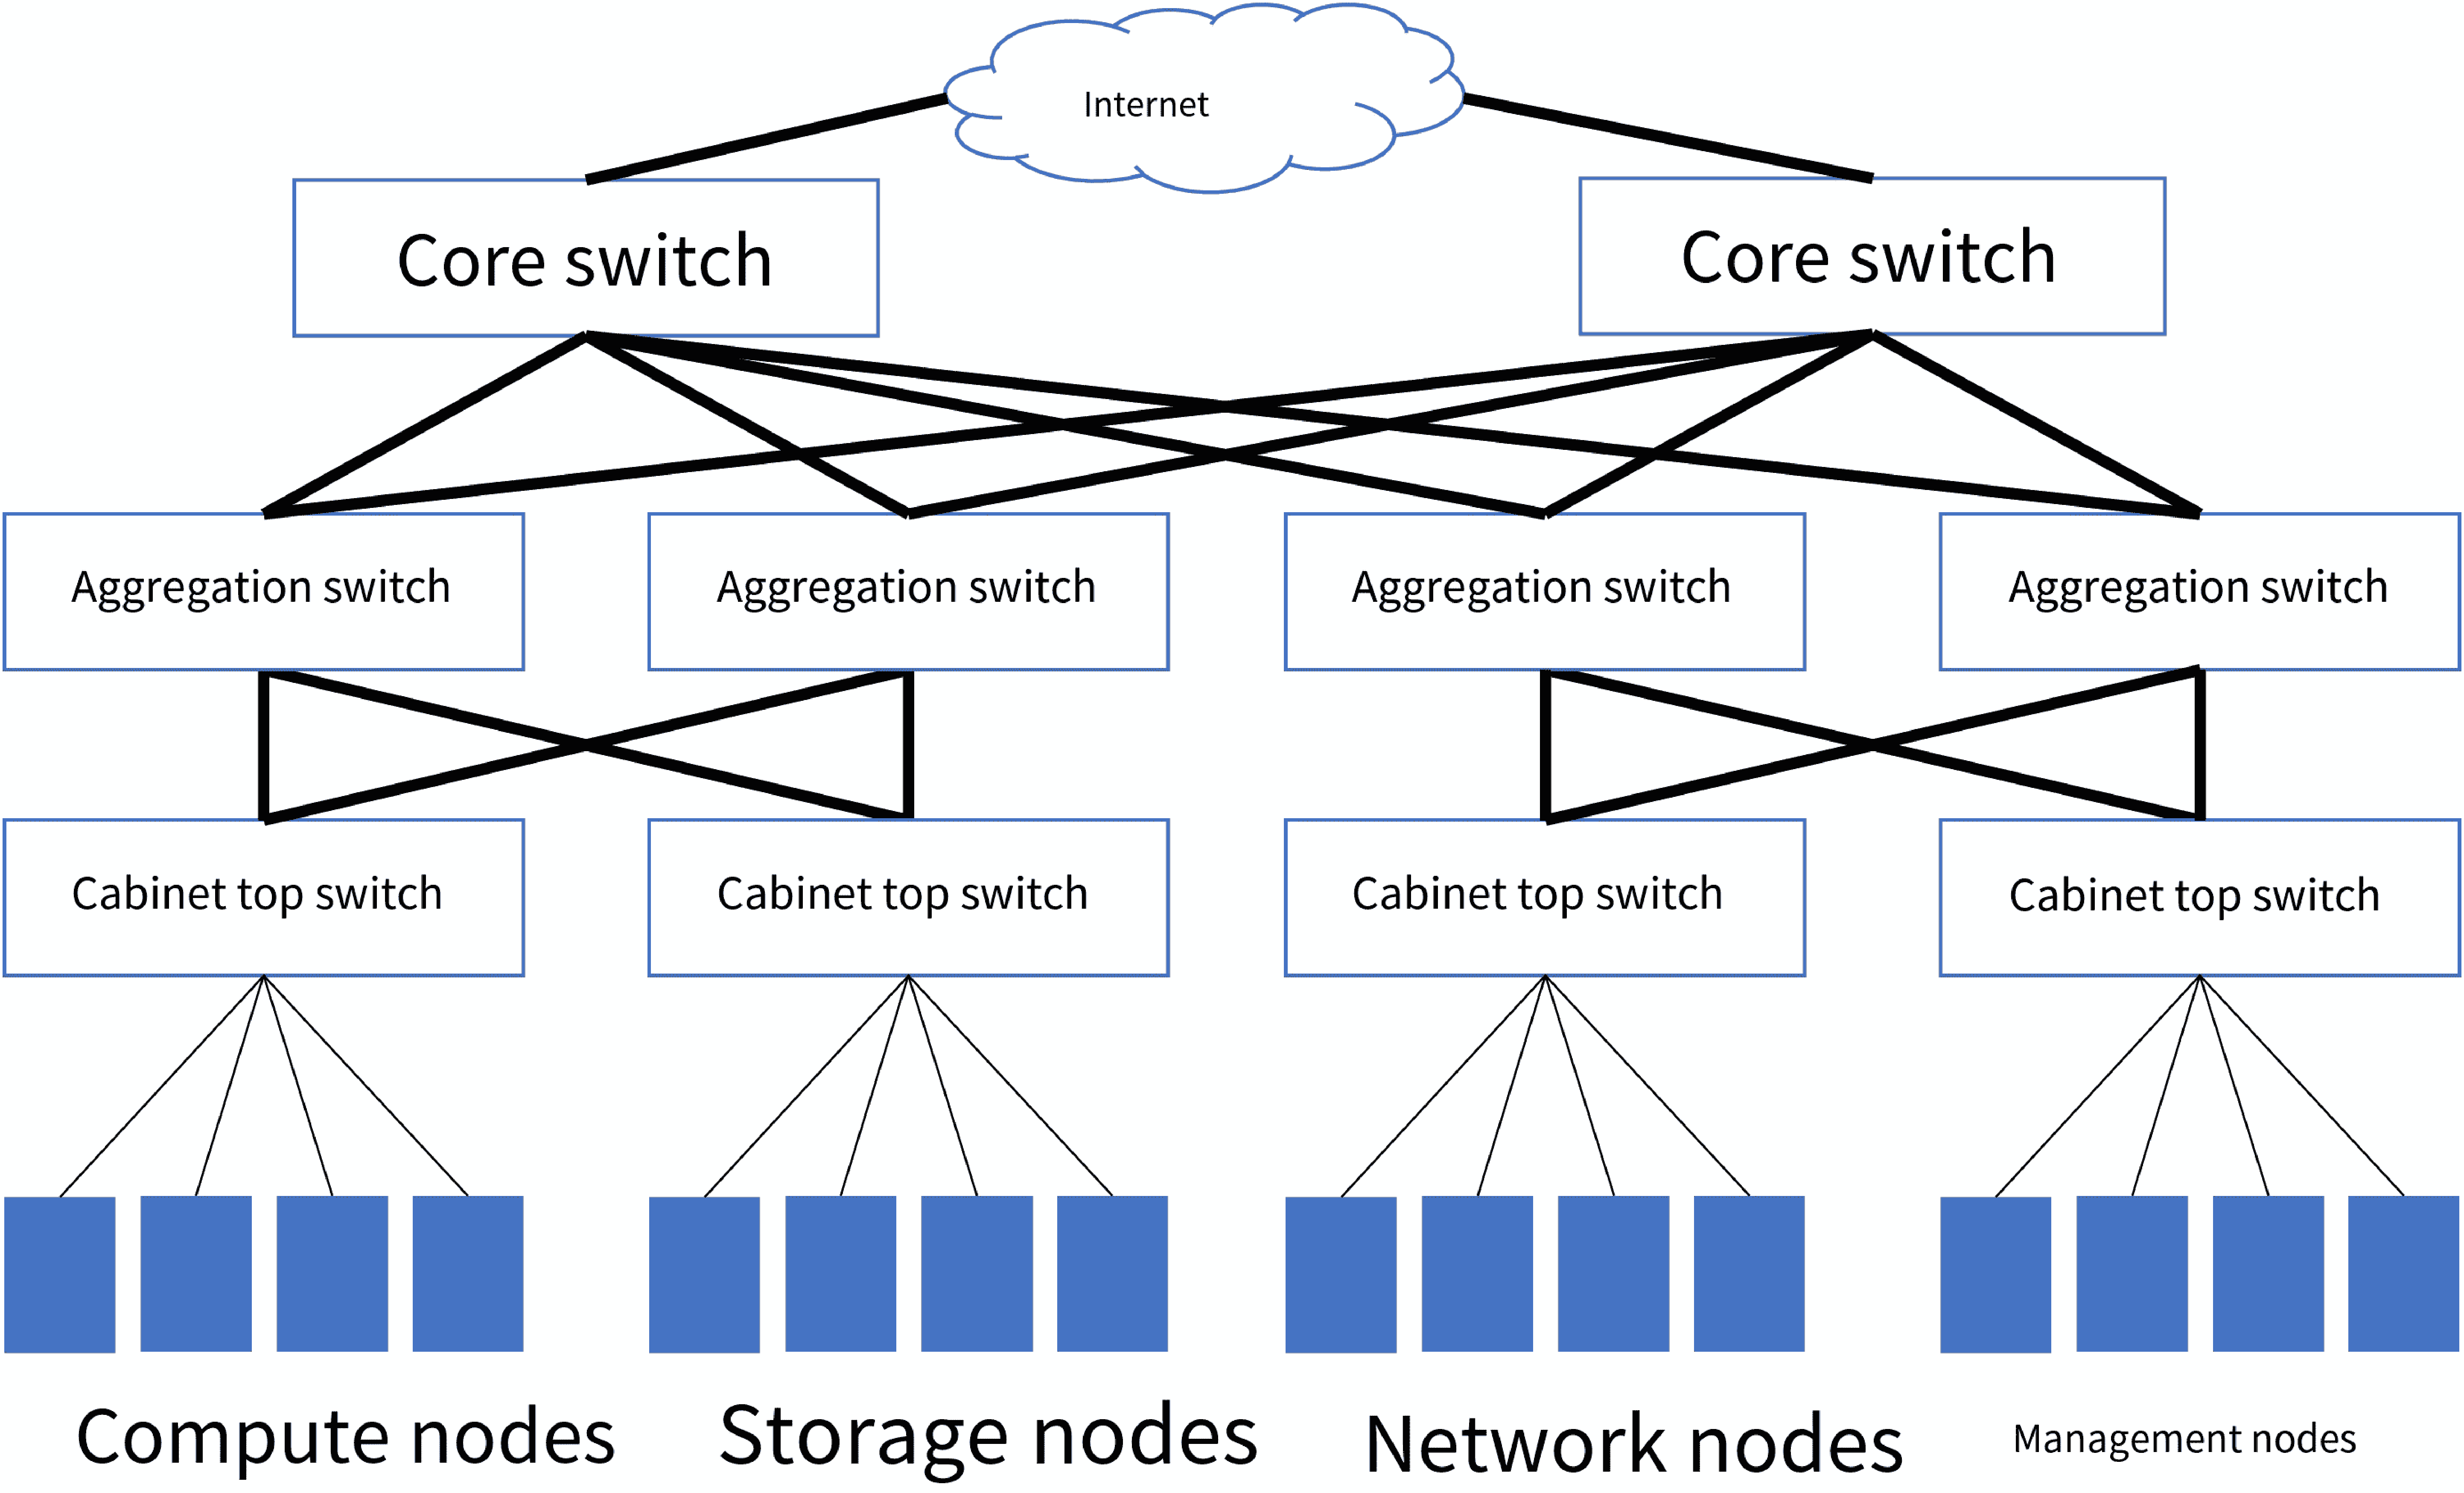
\includegraphics[width=0.6\textwidth]{figures/DC_arch.pdf}
	\caption{数据中心架构。}
	\label{background:fig:cloud-architecture}
\end{figure}

\begin{figure}[htbp]
	\centering
	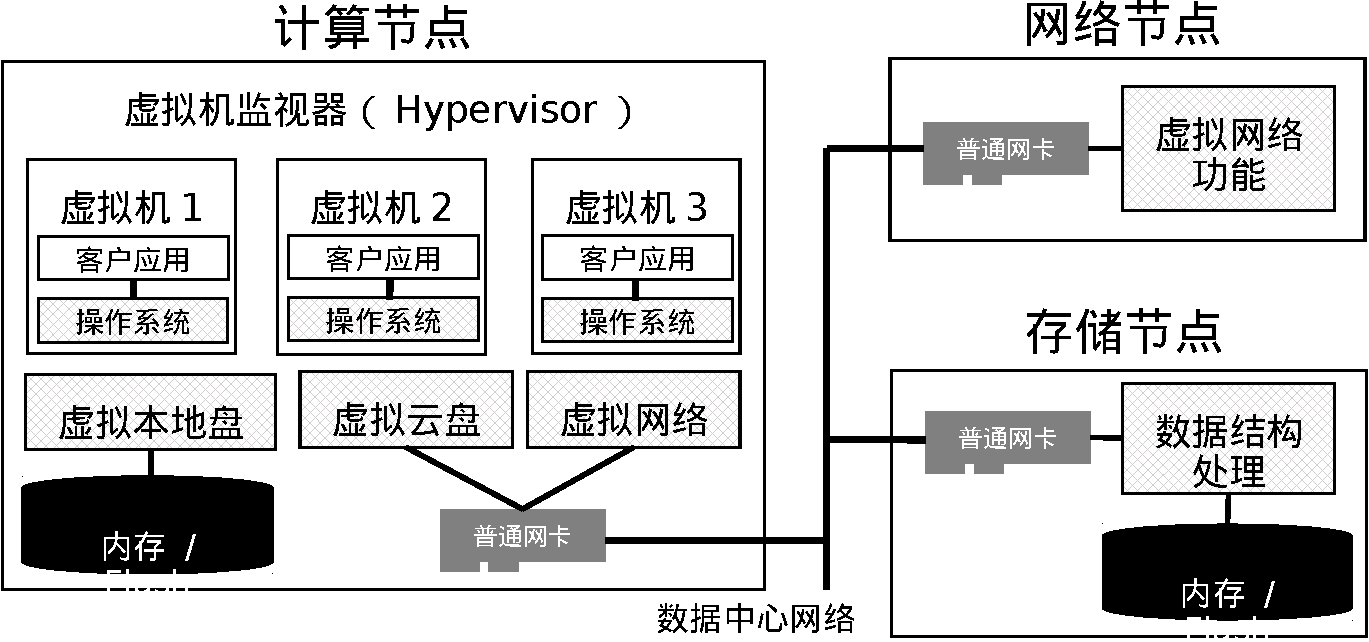
\includegraphics[width=0.8\textwidth]{figures/virt_arch.pdf}
	\caption{虚拟化的数据中心架构。}
	\label{background:fig:virt-architecture}
\end{figure}


\subsubsection{虚拟网络}

除销售虚拟机外,销售基础架构即服务(IaaS)的云供应商必须提供丰富的网络语义,例如具有客户提供的地址空间的私有虚拟网络,安全组和ACL,虚拟路由表,带宽计量,QoS等。 

计算节点上虚拟网络的数据面可以用匹配-操作表(Match Action Table)来描述,理论上可以在商用网络交换机上实现。
2007 年,斯坦福大学提出的 OpenFlow \cite{mckeown2008openflow} 统一了不同厂商交换机的控制面接口,从而可以用软件来对网络进行编程,即软件定义网络(Software Defined Networking,SDN)。
为了支持软件定义网络的控制面,Onix \cite{koponen2010onix} 提出了一个大规模交换机的控制框架,Frenetic 等编程语言 \cite{voellmy2010nettle,foster2011frenetic} 提出用函数式响应型编程(Functional Reactive Programming,FRP)的范式简化控制面事件处理,Covisor \cite{jin2015covisor} 实现了控制面的虚拟化。
随着交换机的可编程性越来越高,用软件自顶向下地定义交换机的数据面转发行为成为可能,而不是像 OpenFlow 那样自下而上地适配交换机的固定功能。

为此,2013 年,斯坦福大学提出了 P4 \cite{bosshart2014p4},提供可编程的数据包解析、有状态的匹配-操作流水线等编程抽象。
学术界提出了 P4 语言在可编程交换机芯片 \cite{bosshart2013forwarding}、可编程网卡 \cite{kaufmann2016high}、FPGA \cite{wang2017p4fpga}、CPU 虚拟交换机 \cite{shahbaz2016pisces} 上的多种实现。
工业界的 Barefoot Tofino 交换机芯片 \cite{barefoot-tofino}、Mellanox Connect-X 网卡 \cite{mellanox}、基于 FPGA 的 Xilinx SDNet 网络处理器 \cite{xilinx-p4} 等也支持了 P4 语言。

然而,基于网络交换机的虚拟网络在云数据中心中有两个根本挑战。
首先,虚拟网络的语义非常复杂,而且变化太频繁,以至于固定功能的传统交换机硬件更新的速度很难匹配需求变更的速度。
其次,一台柜顶交换机连接了数十台机架服务器,一台机架服务器又可以虚拟化出数十台虚拟机,因此交换机需要支持至多上千台虚拟机的数据面封装和转发规则,现有商用交换机芯片的查找表容量不足。
为此,微软提出了类似 P4 的 VFP 编程抽象 \cite{firestone2017vfp} 以支持基于主机的软件定义网络,在虚拟交换机软件中实现虚拟网络。基于主机的虚拟网络可以很好地随计算节点服务器的数量扩放,并保持了物理网络的简单性。

在这种基于虚拟交换机的网络虚拟化模型中,进出物理设备的所有网络I / O都专门在管理程序的主机软件分区中执行。 VM发送和接收的每个数据包都由主机网络堆栈中的虚拟交换机(vSwitch)处理。 接收数据包通常涉及管理程序将每个数据包复制到VM可见缓冲区,模拟到VM的软中断,然后允许VM的OS堆栈继续进行网络处理。 发送数据包类似,但顺序相反。 与非虚拟化环境相比,这种额外的主机处理:降低性能,需要对权限级别进行额外更改,降低吞吐量,增加延迟和延迟变化,并提高主机CPU利用率。

如图 \ref{background:fig:network-perf-trend} 所示,数据中心网络性能的提升速度远远超过通用处理器,在 10 Gbps 网络中只需要一个 CPU 核,而在现在的 40 Gbps 网络中就需要 5 个左右的 CPU 核,而在未来的 100 Gbps 网络中甚至需要 12 个 CPU 核。这就带来了 ``数据中心税''。





\begin{figure}[htbp]
	\centering
	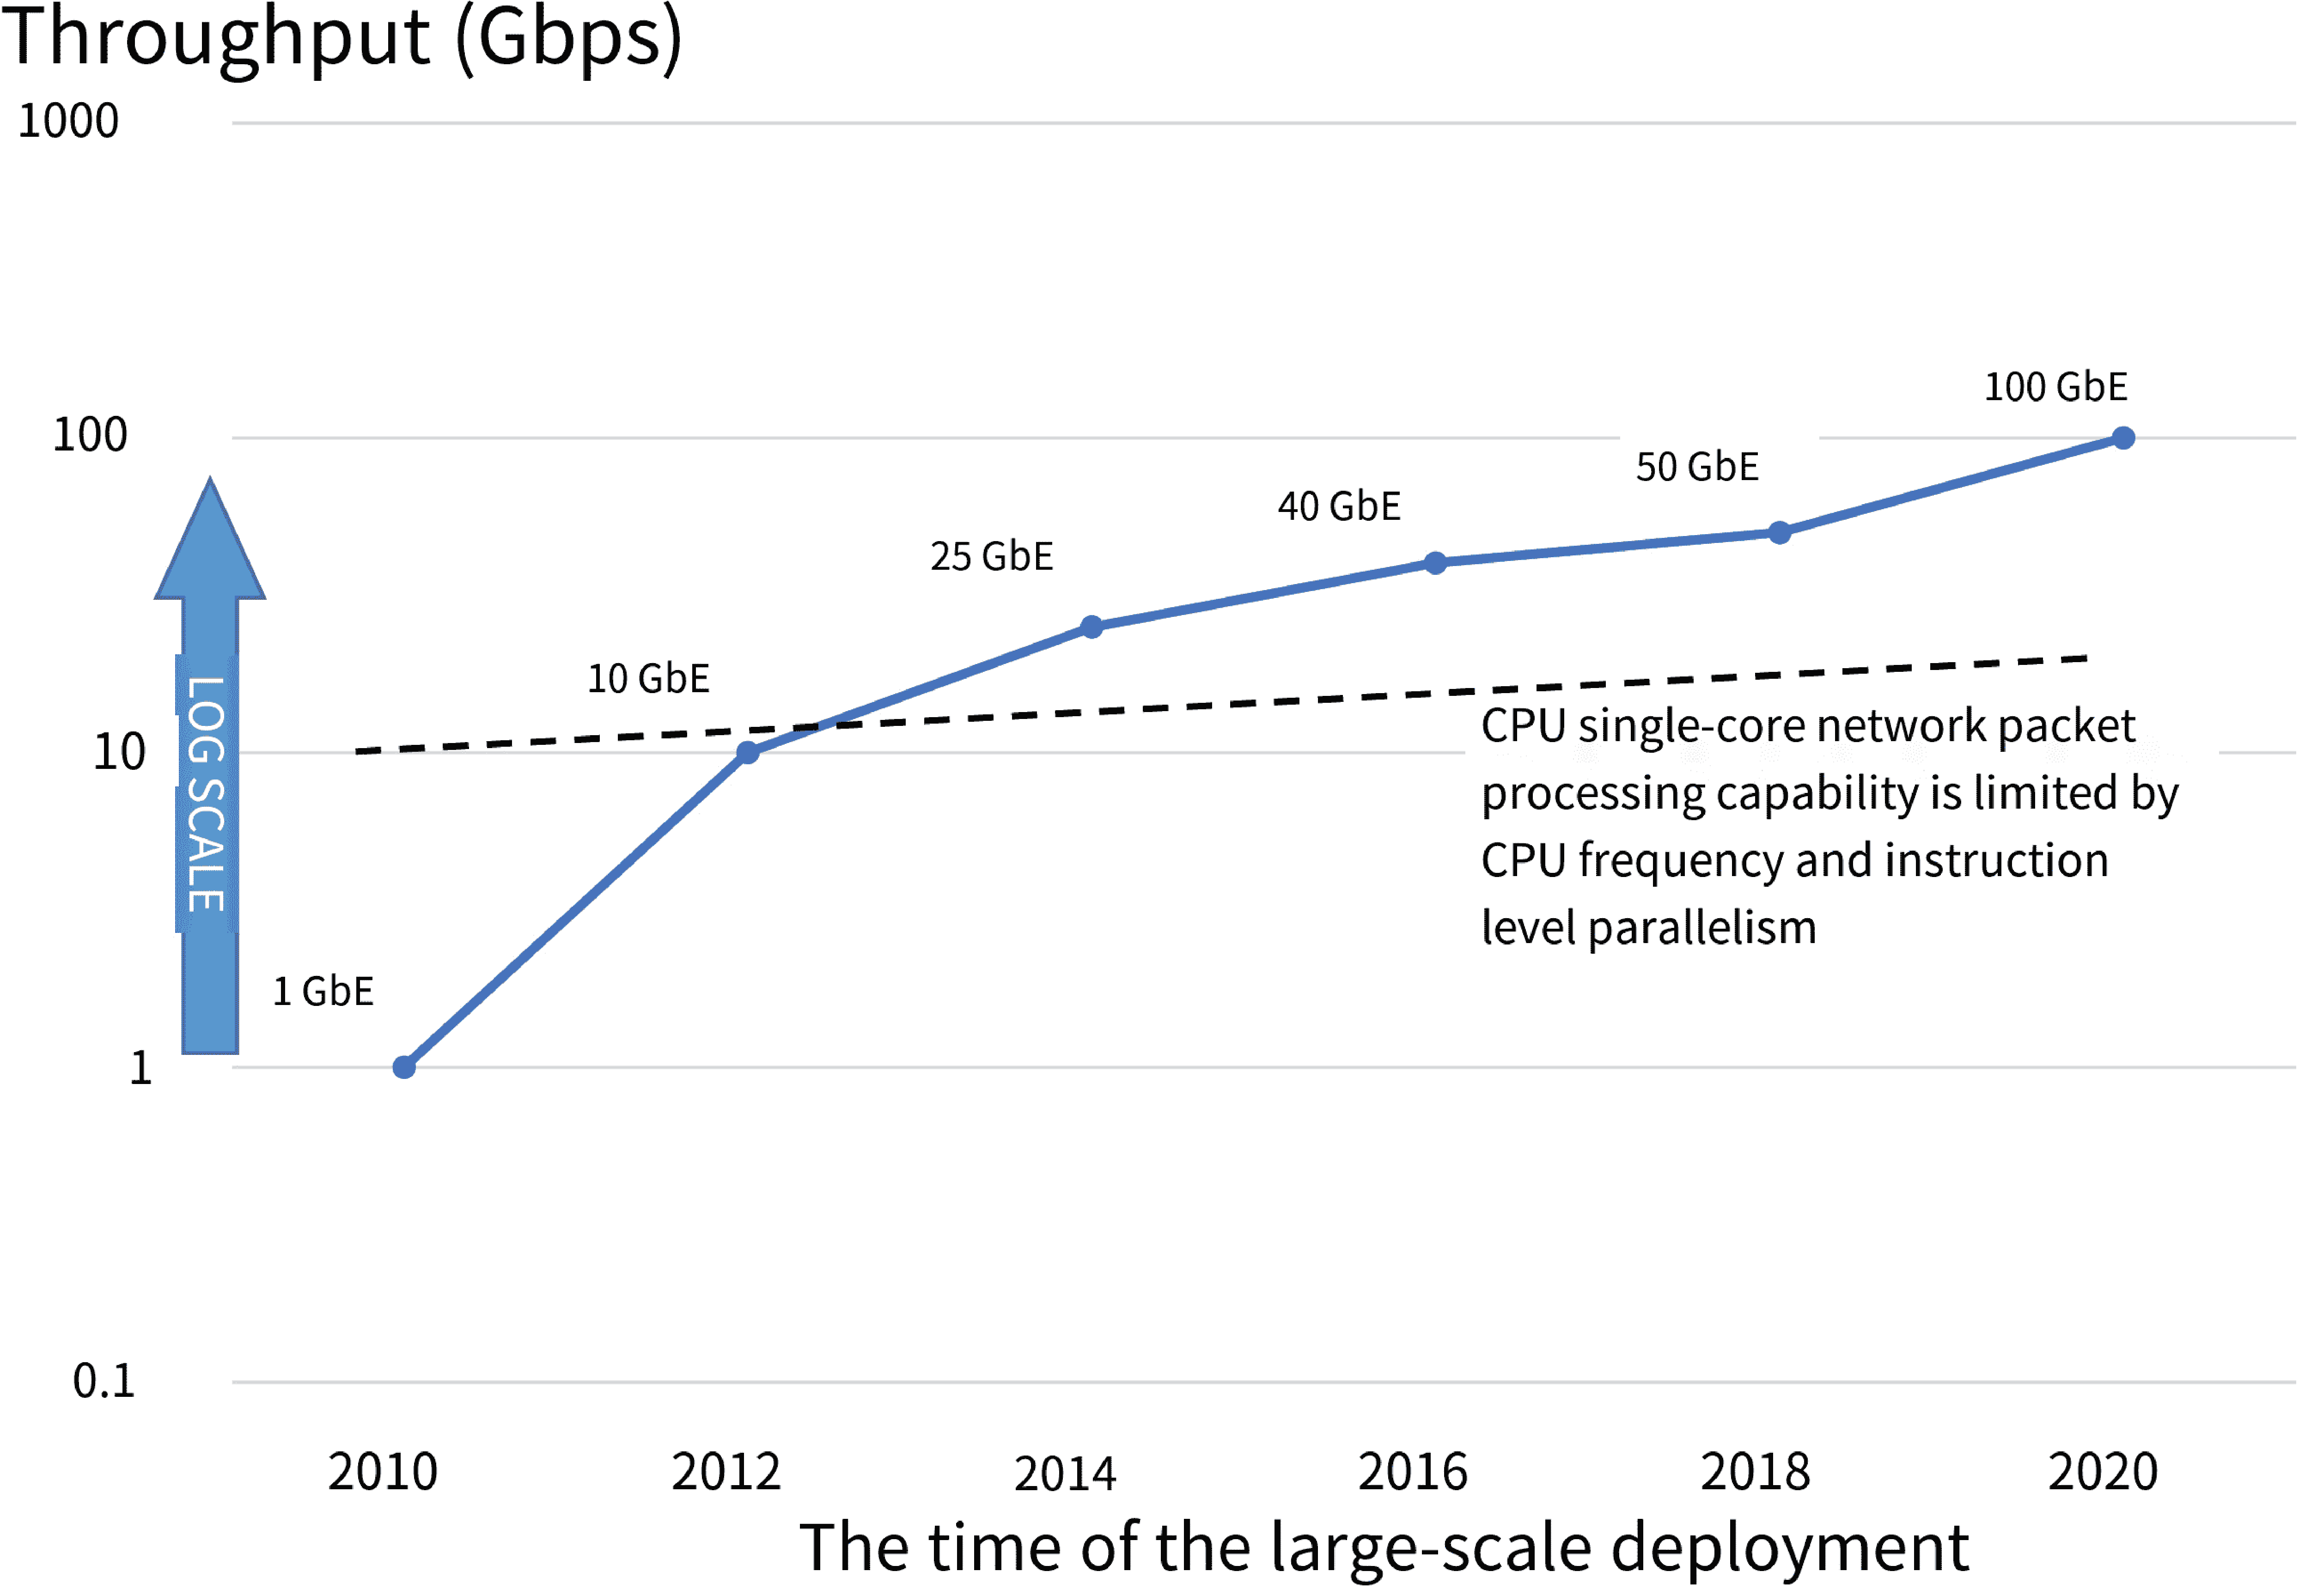
\includegraphics[width=0.6\textwidth]{figures/network_perf_trend.pdf}
	\caption{数据中心网络性能的提升速度远超 CPU。}
	\label{background:fig:network-perf-trend}
\end{figure}


\subsubsection{网络功能}

如图 \ref{background:fig:network-architecture} 所示,两个计算节点上的客户虚拟机之间通信时,经常需要经过一系列网络功能。相比计算节点上的虚拟网络,网络节点上的网络功能就复杂得多。

例如,可扩展的L4负载平衡器 \cite{ananta}

P4 的编程灵活性不足以实现。


\begin{figure}[htbp]
	\centering
	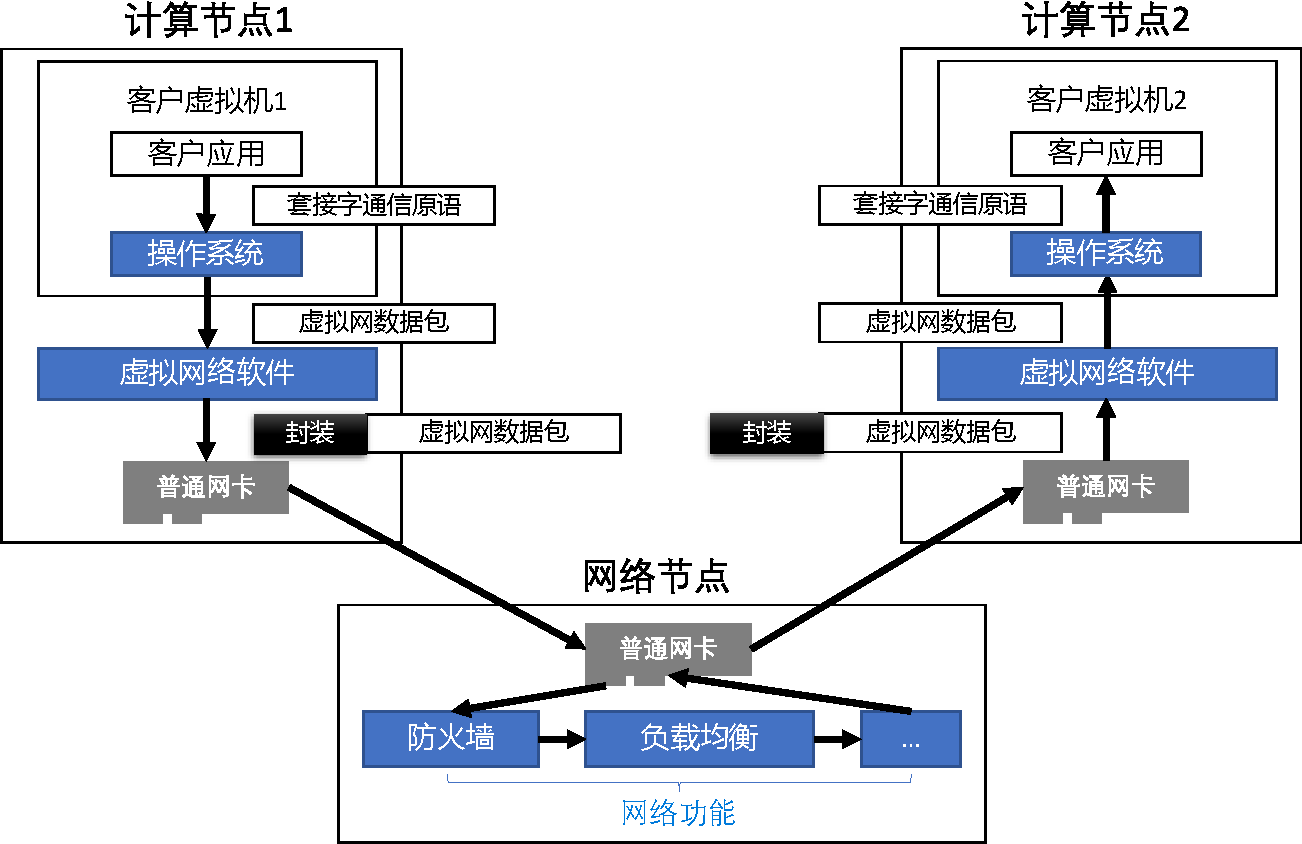
\includegraphics[width=0.8\textwidth]{figures/VPC_arch.pdf}
	\caption{数据中心虚拟网络架构。}
	\label{background:fig:network-architecture}
\end{figure}




Click \cite{kohler2000click} 提出了模块化的网络编程框架。近年来,ClickOS \cite{martins2014clickos} 和 NetBricks \cite{netbricks} 提出了基于 CPU 的

E2 \cite{palkar2015e2} 网络功能

\subsubsection{虚拟存储}




\begin{figure}[htbp]
	\centering
	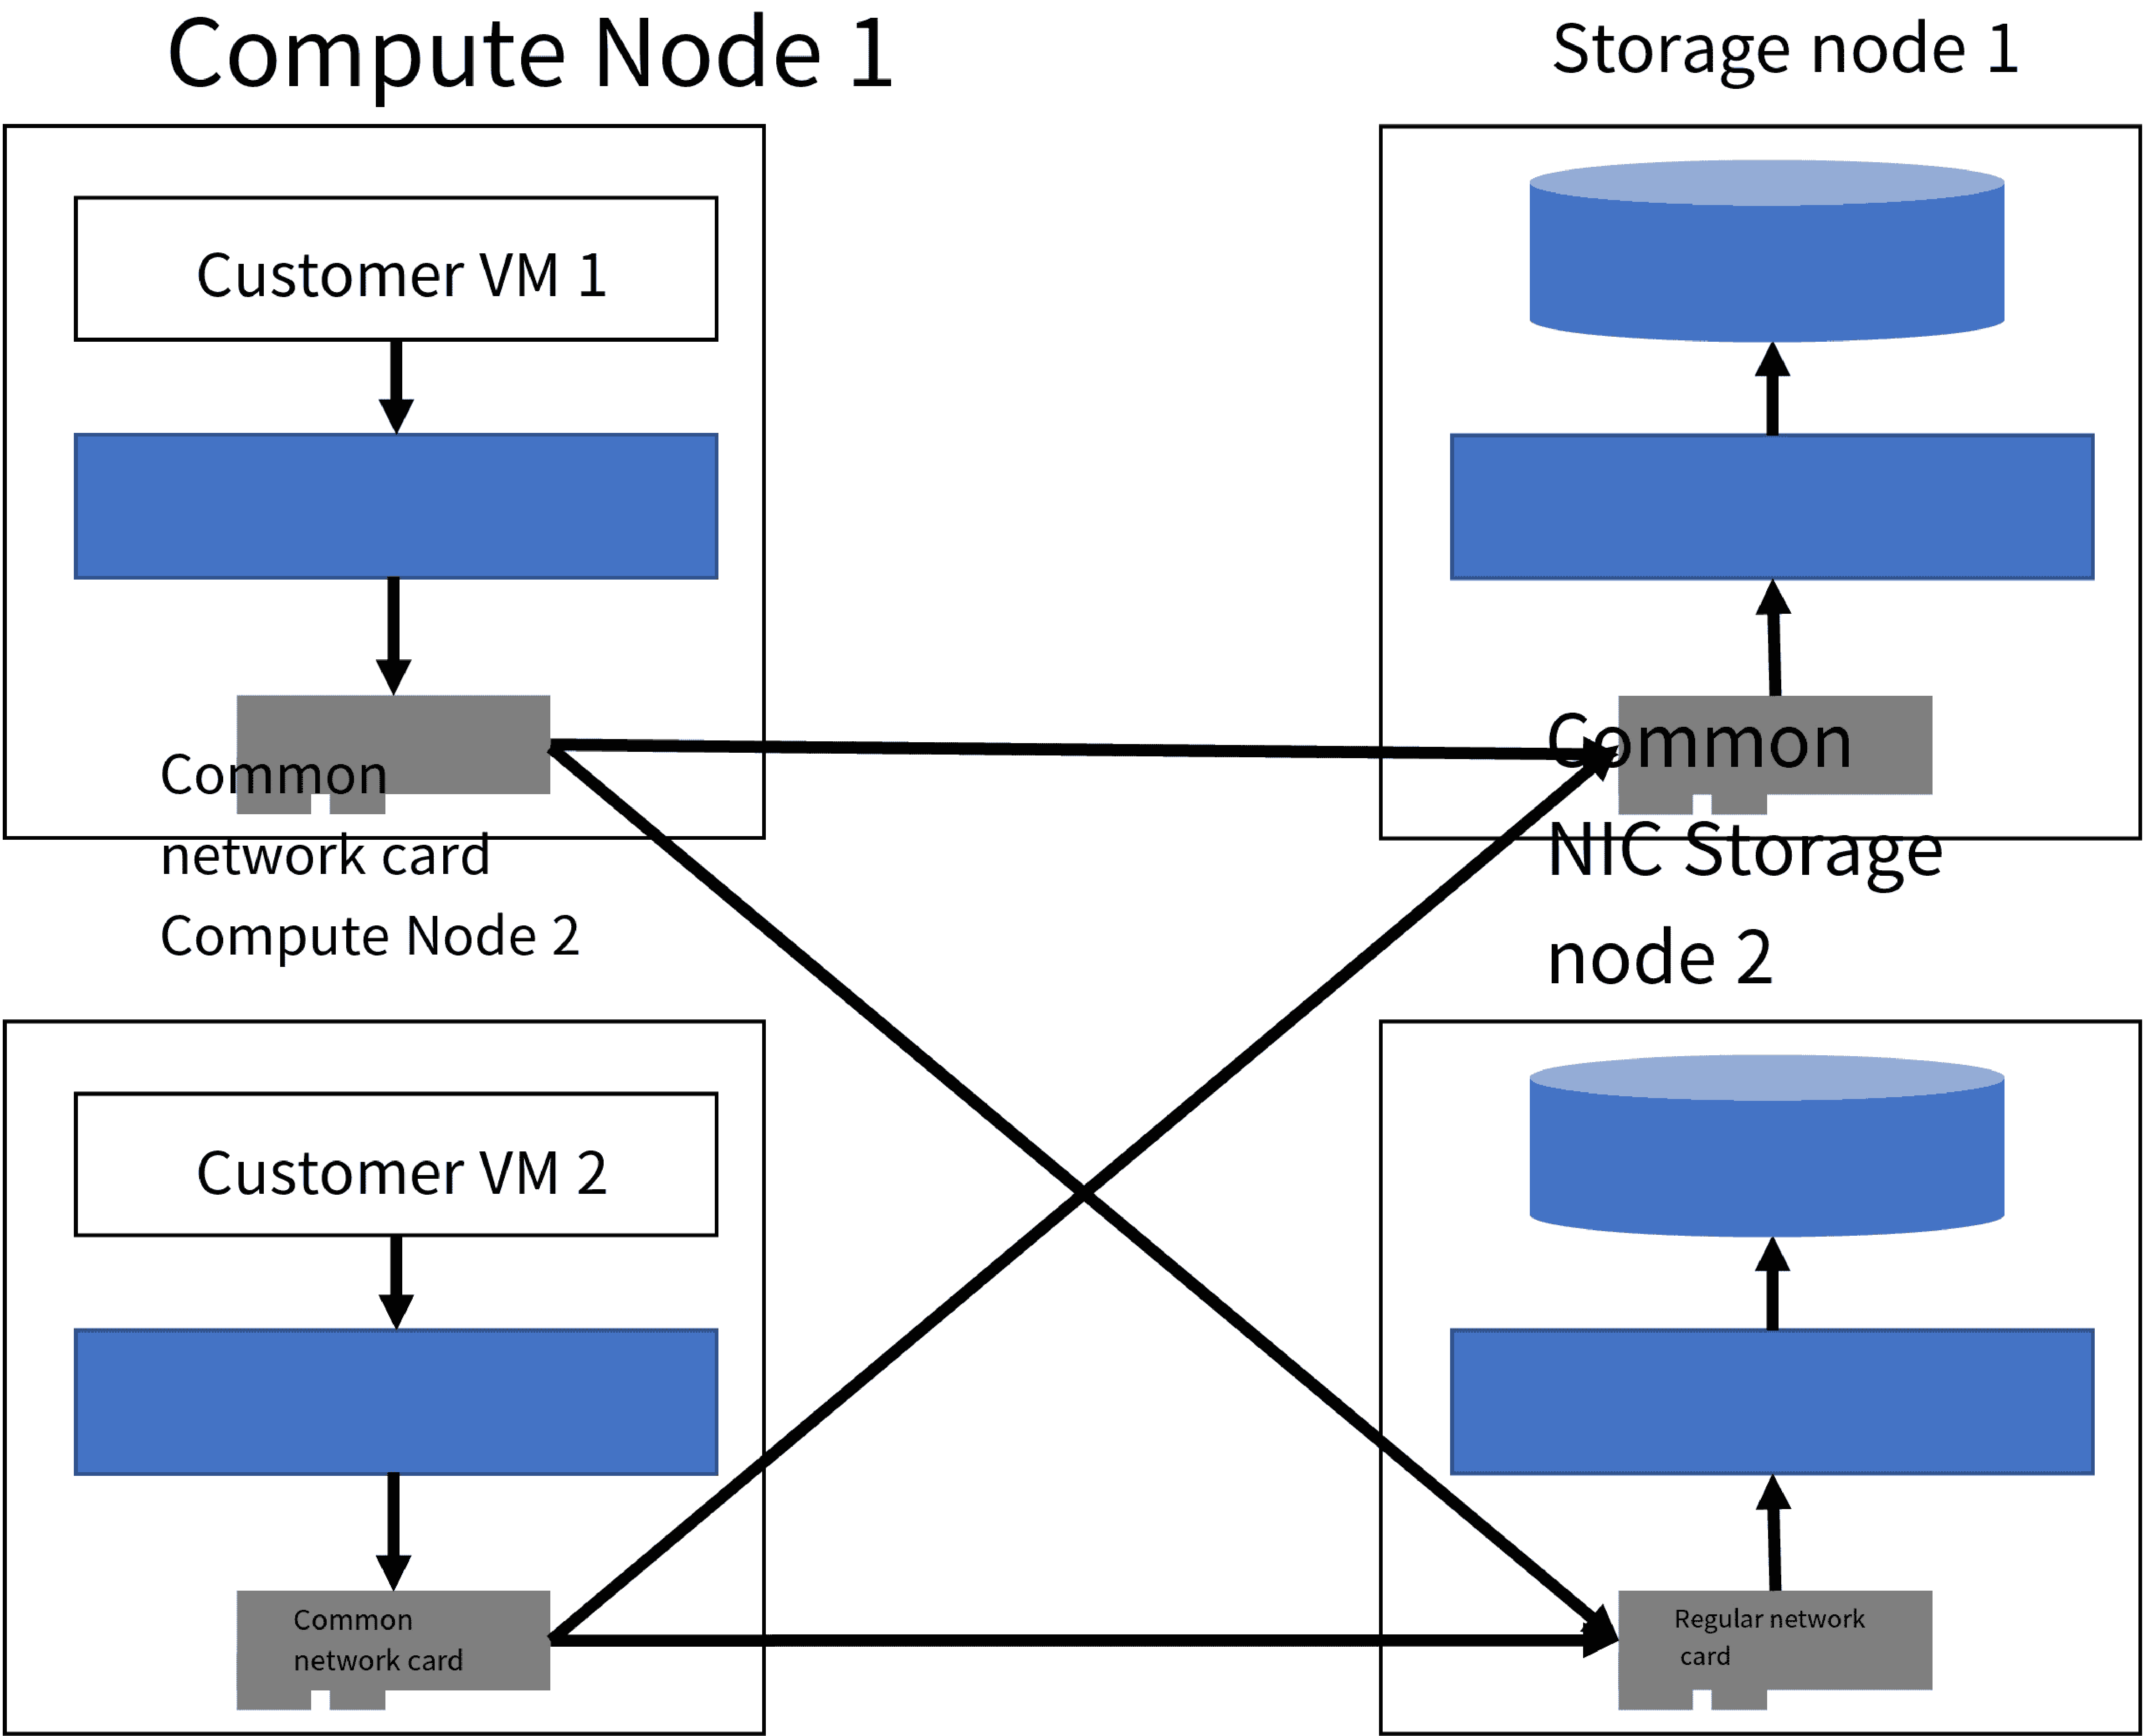
\includegraphics[width=0.6\textwidth]{figures/storage_arch.pdf}
	\caption{数据中心云存储的简要架构。}
	\label{background:fig:storage_arch}
\end{figure}

块存储,本地盘

对象存储,文件存储

临时存储(Serverless computing)

由于云存储的物理存储跟计算节点是分离的,需要把数据从存储节点通过网络搬运过来,还要进行压缩和加密。




\subsection{数据中心功耗的挑战}

如今的一个大型数据中心可以占据几个足球场的面积,容纳数十万台服务器,消耗几十甚至上百兆瓦的电力,相当于一个小型工业城镇的耗电量。据统计,2018 年全球数据中心约消耗 416 太瓦时的电力,相当于 2\% 左右的全球电力能源 \cite{datacenter-energy},占整个信息与通信产业(ICT)能耗的约 33\%。据预测,2025 年,信息与通信产业将消耗 17.8\% 至 20.7\% 的全球电力能源,其中数据中心占 43\% 至 58\% \cite{power-consumption},这意味着 2025 年数据中心将消耗全球电力的约 10\%。因此,数据中心的性能与效率不仅关系到互联网公司的资产和运营成本,还关系到信息产业的未来。

为什么能源问题对信息产业的未来如此重要呢?
1961 年,钱学森预言,``长远以来人们就有在宇宙空间飞行的愿望……星际航行将是科学技术在 20 世纪后半叶中最突出的成就。'' \cite{qianxuesen}
可惜,不同于钱老等大科学家和阿瑟·克拉克等大科幻作家的预言,星际航行的探索尽管推动了众多科学和工程技术的大发展,但由于能源和材料的限制,至今没有成为一项大众技术。
而信息和通信技术(ICT)由于摩尔定律所预言的指数级性能提升,成为 20 世纪末以来最为耀眼的科技新星。

由于信息是无形的,我们可以通过把信息的存储和处理单元做得越来越小来提升单位面积集成电路的存储和处理单元数量,从而提升单位面积集成电路的性能。这也是摩尔定律的原始表述。
更为深刻的是 Dennard 缩放定律 \cite{dennard1974design},即集成电路的性能在不消耗更多能源和面积的情况下能够每两年翻倍。
它的理论基础是每两年采用一代新的半导体工艺,晶体管尺寸缩小 30\%,从而芯片面积缩小 50\%。为了保持电场的恒定,电压随晶体管尺寸同比例降低了 30\%。与此同时,由于芯片尺寸缩小了,延迟降低了 30\%,时钟频率就可以提升 40\% \cite{borkar1999design,borkar2011future}。
在那个年代,集成电路的动态功耗占了功耗的主要部分,其与电容、电压的平方和频率成正比,从而可以计算出功耗降低了 50\%。
按照这个理想模型,每两年集成电路的面积和功耗都减半,就可以在原有的面积和功耗下塞进两倍数量的晶体管,而且时钟频率还提高到了 1.4 倍。
对于冯·诺伊曼体系结构的单线程微处理器,这些增加的晶体管主要用于更大的缓存、更复杂的流水线、超标量、乱序执行、寄存器重命名、分支预测等,以提高每时钟周期所能执行的指令数。
根据 Pollard 经验定律 \cite{pollackpollack},每时钟周期的计算能力大约与晶体管数量的平方根成正比。
单位时间的算力等于时钟频率乘以每时钟周期的算力,因此每两年微处理器的性能提升到 2 倍,还不消耗更多的能源和面积。

信息系统性能提升的速度在处理宏观有形物体的其他行业是难以想象的。
1976 年,协和式客机的速度就突破了音障,然而它因为油耗太高而没有经济性。现代客机与 50 年前的多数客机一样,仍然以亚音速飞行。
而从普速火车到高铁的大量系统创新,也只把运营速度提高到了 2 倍多。
目前,人类的主要能源来源是化石能源,由于其使用成本和环境影响,在新能源技术取得重大突破前,能源仍然是各行各业发展的重要制约因素 \cite{energy}。
相比数据中心,移动终端和物联网设备对功耗更敏感,因为电池的能量密度提升缓慢,而这些设备对体积和重量很敏感。

不幸的是,进入 21 世纪以来,摩尔定律和 Dennard 缩放定律的红利正在逐渐消失。
首先,随着集成电路特征尺寸的缩小,电压也随之降低。但控制晶体管的阈值电压越低,晶体管的漏电流就会迅速增长,成为集成电路功耗的重要组成部分。
为了控制漏电流,阈值电压不仅不能降低,甚至需要比前一代集成电路有所提高 \cite{borkar1999design}。
因此,每一代新的半导体工艺,每晶体管的功耗不会像预期的那样降低一半。
其次,由于每晶体管的面积缩小一半,功耗却没有降低这么多,单位面积集成电路的功耗就会升高。
目前 100 平方毫米芯片的功耗大约是 65 瓦 \cite{borkar2011future},成为人类最高功率密度的可控设备之一,单位体积的功率密度甚至与航空发动机相当。因此,芯片的散热问题成为制约集成电路规模的主要因素。
再次,对于同一个集成电路,在允许的范围内,为了提高一倍的性能而把时钟频率提高一倍,电压就要相应提高一倍来降低晶体管的翻转延迟,因此功耗大致与时钟频率的三次方成正比。
由于散热的限制,集成电路的时钟频率也受到限制,靠 ``超频'' 来大幅提升集成电路性能是不现实的。
最后,目前 7 nm 半导体工艺已经量产,而硅原子的半径为 0.1 nm。
随着集成电路的特征尺寸越来越接近原子尺寸,量子效应不可忽略,给光刻技术带来了很大的技术挑战 \cite{borkar2011future}。
事实上,约 2010 年以来,集成电路特征尺寸的缩小已经明显放缓,不再能保持两年一代的速度。
综上,在当前的半导体技术框架下,单位面积集成电路的性能已经不再能维持两年提升一倍的速度,而且性能的提升也意味着功耗的提升,``免费的午餐'' 结束了。

在通信技术方面,信道编码从相对低效的汉明(Hamming)码和格雷(Golay)码,发展到卷积码,再到接近香农极限的 Turbo 码和从故纸堆中翻出来的 LDPC 码,以及理论上达到香农极限的 Polar 码,在物理信道和信噪比不变的前提下,通信系统的吞吐量逐渐接近香农极限。
事实上,Turbo 码在 HSPA、LTE、WiMAX 等无线通信标准中被广泛采用,LDPC 码被用于 5G eMBB 数据信道、IEEE 802.11n 无线局域网、WiMAX 等,Polar 码也被用于 5G eMBB 控制信道等。
现代无线通信系统的性能提升已经不再主要依靠信道编码的改进,而是主要依靠带宽更高的物理信道、MIMO、改进的多址技术、改进的信道估计和干扰管理、中继等空中接口技术,以及核心网的云化和微服务化。其中的很多环节依赖于计算性能的提升,例如 5G 核心网数据面处理的延迟和吞吐量要求都显著提高,MIMO 等技术也增加了很多计算量,因此仍然受制于集成电路的性能。
如果计算、存储和通信系统的性能只是依靠消耗更多的能源和材料线性增长,显然是既不经济又不可持续的。

\subsection{性能优化的空间}

在摩尔定律和 Dennard 缩放定律的红利逐渐消失的今天,我们是否可以继续提升计算、存储和网络的性能,维持信息产业的高速发展呢?
答案是肯定的。
从远期来看,量子计算、DNA 存储 \cite{bornholt2016dna}、光存储 \cite{glass-a-new-media-for-a-new-era}、光交换 \cite{farrington2011helios} 等新技术有无限可能。
从近期来看,基于半导体集成电路的当前计算机系统性能还有大量的可优化空间,我们还有机会 ``从摩尔定律这个柠檬里又榨出这么多汁来'' \cite{threebody},这也是本文关注的重点。

首先,从芯片的体系结构角度看,传统的冯·诺伊曼体系结构并不能充分利用每个晶体管的计算能力。
理论上,每时钟周期的算力可以与晶体管数量成正比,但前述的 Pollard 经验定律 \cite{pollackpollack} 指出,每时钟周期的算力事实上是与晶体管数量的平方根成正比。
例如,1971 年的全球第一款微处理器 Intel 4004 使用 10 微米制程,有 2300 个晶体管,时钟频率 108 KHz,每秒能执行 90 K 次 4 位运算。
2016 年 Intel 基于 Broadwell 架构的 Xeon E5 微处理器使用 14 纳米制程(4004 的 1 M 倍),有 72 亿个晶体管(4004 的 3 M 倍),基频 2.2 GHz(4004 的 20 K 倍),每秒能执行约 300 G 次 64 位运算 \footnote{假设应用使用 AVX2 指令,不使用 FMA3 指令,没有超频。}(4004 的 3 M 倍) \cite{intel-e5-v4}。
可以看到,Xeon E5 每时钟周期能执行的运算数是 4004 的约 150 倍,而晶体管数是 300 万倍。即使考虑到 64 位计算比 4 位计算复杂的因素,仍然意味着 4004 每个晶体管对算力的贡献比 Xeon E5 高数百倍。
这是由于冯·诺伊曼结构微处理器的指令集和微体系结构越来越复杂,一方面是为了提高单线程性能、添加更深的缓存层次来解决 ``内存墙'' 问题,另一方面是为了支持多核间的通信与同步、操作系统和虚拟化技术,真正用于计算的晶体管占比越来越少了。

\begin{figure}[htbp]
	\centering
	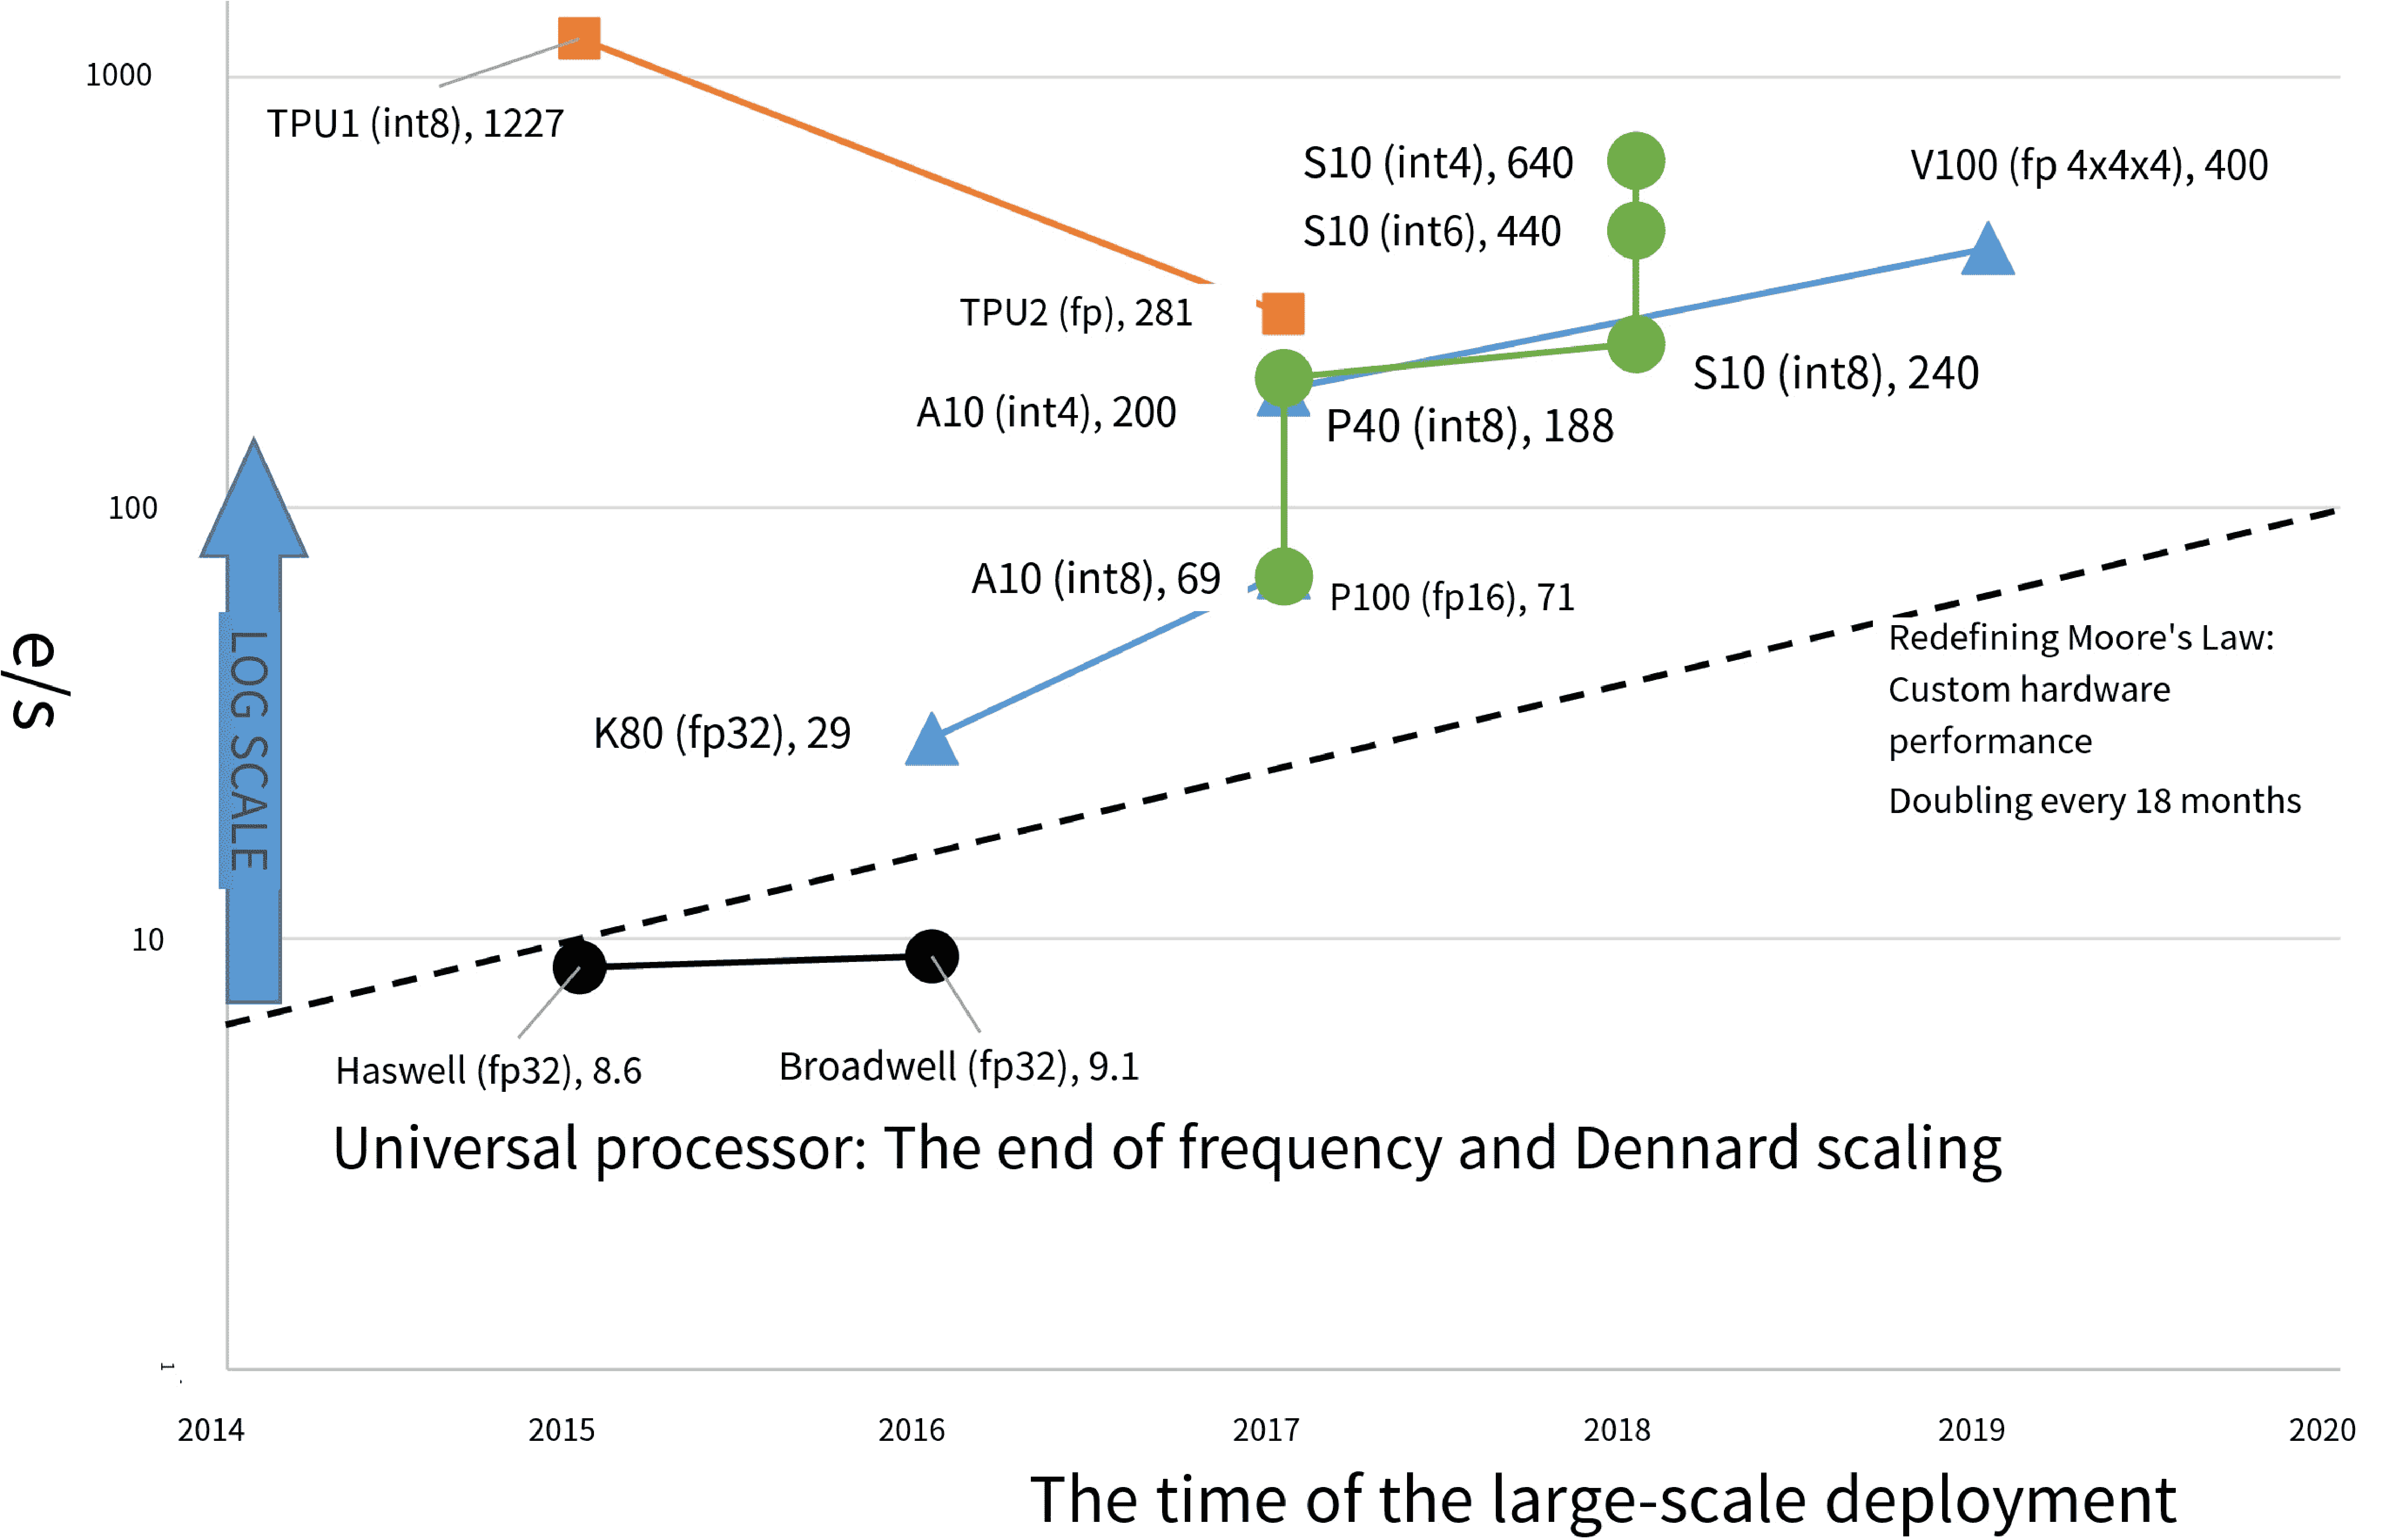
\includegraphics[width=0.8\textwidth]{figures/moores_law_redefined.pdf}
	\caption{通用处理器的频率和 Dennard 缩放逐渐终结,但定制化硬件重新定义并延续了摩尔定律。}
	\label{background:fig:moores_law_redefined}
\end{figure}

第二,操作系统,大量开销,数据中心税。

第三,软件开发,安迪比尔定律。

第四,数据中心层面:大部分物理服务器的使用率只有大约10\%到15\%,但是功耗却与使用率最高时相差无几。云为什么需要热迁移?


\iffalse

\subsection{芯片的发展}

计算机体系结构的进步是和半导体集成电路的发展分不开的。可以毫不夸张地说,计算机的发展是集成电路技术最大的推动力,也是最大的获益者。过去半个多世纪以来,集成电路一直大致保持着摩尔定律预测的速度发展,高度集成的芯片带来一次又一次计算机体系结构的革命,从巨型机(MainFrame)到个人电脑(Desktop),从服务器到云计算平台,从笔记本电脑到移动计算,集成电路使得各种形态的计算机快速地渗透到我们生活的方方面面。而另一方面,正是计算的需求,推动了中央处理器 (CPU),内存 (DRAM),图形加速器 (GPU) 以及高速网络芯片的发展。芯片技术和计算机体系结构相辅相成,共同推动了计算机系统软件和计算机应用的发展,使信息技术在短短的几十年中获得了如此重要的社会和经济地位。

目前信息科学技术依然处于一个高速发展的阶段,新的应用层出不穷:人工智能、物联网、虚拟现实、区块链,新兴的方向让人目不暇接,每一项技术都有无穷的潜力,可能推动人类社会进入全新的未来。而另一方面,基于半导体硅的CMOS集成电路芯片技术由于受到物理规律的限制,已经开始达到瓶颈。一方面芯片的线宽(Feature Size)在5纳米以下已经很难进一步缩小,而另一方面功耗和散热已经成为现代芯片技术难以绕过的难题。在这种情况下,计算机技术会何去何从?未来的计算机如何满足不断增长的计算能力的需求?

借助这篇短文,我们想探讨一下我们认为计算机系统在未来几年中发展的可能方向,尤其是集成电路技术如何与计算机体系结构继续相互推动,提高计算的速度和效率,满足不断增长的算力需求。目前学术界和工业界的共识是,科学家们看来不太可能找到短期内能代替CMOS的技术,计算机技术性能的提升在短期内必须主要依靠计算机体系结构的创新。在这篇短文里,我们着重探讨一下云计算平台的体系结构可能的发展趋势和方向。在可以预见的未来,云计算会是非常重要的计算平台,它会提供人类社会主要的算力,推动整个世界的数据处理能力。当然,移动计算、物联网以及其它“端”也是非常重要的发展方向,但限于篇幅,在这篇短文中我们就不详细探讨这些方面的发展。

\subsection{云计算平台的变革}

在21世纪初期,云计算的概念刚刚起步的时候,云计算的平台基本上就是一个普通的企业数据中心,只不过规模比较大而已。当时的云计算与传统意义上科学计算用的超算平台在硬件上有很大区别。科学计算用的超级计算机往往使用定制的芯片,定制的网络,不惜成本地追求最高的性能。而云平台的特点就是把普通的低端商用服务器规模化,用软件实现高容错、高可靠性,降低成本,提供高性能的服务。

随着云计算商业模式得到用户的认可,特别是公有云的概念被广泛接受,经过近二十年的发展,目前主要的云计算平台提供商已经取得了巨大的商业成功。云计算平台的规模已经大大扩张。业界领先的云平台已经拥有遍布世界各地数以百计的数据中心以及数以百万计的服务器。这对计算机的体系结构带来了非常多新的挑战。建设一个大规模的云计算平台需要巨大的投资,任何能够减少单机成本的创新都能带来极高回报;云计算需要大量电力维持运转,提高系统的效率,降低功耗是重要的指标;云计算平台的一个大卖点就是弹性和灵活的配置,如何提供弹性同时尽可能减少系统空闲是一个复杂的问题;云计算需要保证可靠性,需要易于管理,需要保护私有信息,这里有非常多的挑战都需要解决。

在计算机发展的早期,软硬件是由同一个公司团队开发的,许多黑科技在这个大环境下被发明创造出来,对后世产生了深远影响。随着计算机的发展,设计分工变得越来越细,CPU、内存、网络、操作系统等等计算机的组成部分逐渐由各个专业公司独立完成,这使得工程师们必须遵守现有的体系框架,跨界创新变得非常困难。虽然在某些专用领域(例如游戏机)设计师们还可能做系统全盘考虑,但在通用计算领域这几乎成了不可能的任务。


\subsection{可编程逻辑阵列FPGA 和专用集成电路 ASIC}

为了更好了解集成电路和计算机体系结构,需要在这里简单介绍一下两个重要的集成电路技术。

ASIC(Application Specific Integrated Circuit,专用集成电路)是为某些应用专门开发的集成电路芯片。ASIC开发门槛比较高,研发周期也比较长。在目前的技术水平下,中等复杂度的ASIC前期投入的一次性开发成本(NRE, Non-Recurring Engineering)会在数百万到一两千万美元左右,并且需要一两年的开发周期。

FPGA(Field Programmable Gate Array,可编程门阵列)是一种可以重新定制 (reconfigurable) 的集成电路元器件。直观上来说,FPGA就是一个可以用编程的方法重新组合的一大堆电子元器件。这些元器件包括逻辑门(如与,或,非门),寄存器 (Register),加法器,静态内存(SRAM)等等,用户可以定制它们之间的连接从而组成不同的电路。如今的FPGA除了基本元件,还加入了越来越多的DSP和硬核(hard IP),以提高乘法、浮点运算和访问外围设备的性能。FPGA的优点是技术比较成熟,开发门槛相对其它集成电路(如ASIC)较低,部署后依然可以修改,缺点是性能比专用芯片差。

FPGA传统上被广泛应用于原型设计,逻辑电路模拟,以及高端路由器等等的领域。最近几年FPGA开始被在数据中心中得到越来越广泛的应用。在数据中心中,FPGA主要被用在两个方面,一方面是用于部署后依然可能需要改变的应用上,比如网卡。由于公有云的网卡上经常需要调整或添加协议,需要经常对硬件重新编程。另一种应用是计算加速:对于一些特殊的计算,可以利用FPGA可以高度并行化的的特性加速。在数据中心中用FPGA加速应用的一个大概的规则是10,100,1000规则:应用需要可以被加速十倍以上,如果加速比太小就不值得做硬件的实现了;被加速的部分核心大约相当于100行以下的代码,更复杂的逻辑用硬件实现难度就会比较大;而计算在数据中心应该需要至少1000台左右的服务器,如果服务器数目远远小于1000台,可能就不值得开发硬件方案了。当然,这些数字都是非常粗略的估计,应该根据FPGA的部署情况,应用本身的价值,以及开发人员的实际情况做相应调整。

在过去,开发ASIC往往是专业硬件芯片公司才能做到的事情。但随着云计算平台规模的不断扩大,云计算系统公司也开始尝试针对自己的云独立设计专用芯片。
\fi

\section{数据中心硬件的发展趋势}
\label{background:sec:hardware}



现代计算机系统大致可以被划分成四个主要部分:计算系统(Compute)、内存系统(Memory)、存储系统(Storage)以及网络和互连系统(Networking and Interconnect)。


\subsection{计算系统}

计算系统是整个计算机的核心,通常是由中央处理器CPU和一些为特殊应用服务的加速器构成。从整个计算机体系结构的发展来看,计算系统上的创新可能是最受关注的一个领域了。

在过去,计算系统基本上就等同于CPU,而CPU上的创新是由Intel、IBM等少数几个大公司主导的。传统上计算力是计算机系统中相对比较富裕的资源。一方面得益于摩尔定律及CPU体系结构的进步,CPU的速度和效率得到了长足的进步;另一方面其它的子系统例如硬盘,内存和网络因为相对缓慢的进展而往往成为实际应用的瓶颈。这种情况在最近几年发生了很大改变:随着新的硬件如固态硬盘和超高速光通信网络的出现, I/O往往不再是瓶颈;而新的应用如深度学习和内存数据库等对算力有极大需求,传统的CPU已经越来越难以支撑这些应用。正因为如此,在计算系统上创新,也就是大家通常所说的异构系统成为近年来计算机体系结构研究的一个热点。

\subsubsection{深度学习加速器}

最近深度学习的热潮,使得计算加速成为一个热点。从大学到工业界,从初创企业到业界巨头,从传统的半导体公司到传统的应用软件开发商都在尝试设计专门针对深度学习应用的硬件加速器,为小到低功耗的IoT设备,大到整个数据中心设计解决方案。在云计算领域,谷歌作为利用集成电路ASIC加速深度学习的先行者,为此设计的专用张量处理器(TPU)目前已经发展到第3代,无论从技术创新,吸引眼球,还是商业运作方面都取得了极大的成功。微软利用FPGA做深度神经网络(DNN)加速,也已经在Azure云平台上线。

深度学习包括训练和推理两种场景。训练所需的内存大、运算复杂,大多部署在云数据中心,NVIDIA的GPU具有巨大的生态系统优势,仅有第三代TPU、Graphcore等少数深度学习加速器正在挑战其垄断地位。推理的应用场景则较为异构。移动计算场景下低功耗是最重要的需求,如寒武纪神经网络处理器以知识产权(IP)授权的形式集成进入华为麒麟970处理器;搜索推荐、自动驾驶和虚拟现实场景下,既需要毫秒甚至微秒级的低延迟,又需要较高的吞吐量。推理的多种场景下不仅有不同的性能指标,所需的神经网络运算也不尽相同。加速器除了支持循环神经网络、卷积、矩阵乘法、正则化等经典神经网络运算,还需要与场景相关的算法共同演进,利用稀疏化(sparsity)、量化(quantization)等技术在不降低精度的前提下提高算力,并支持动态控制流等新兴的神经网络结构。\textbf{cite 张宸的 paper}

\subsubsection{FPGA和可重构硬件}

用FPGA做计算加速在学术界已经被研究多年,在某些特定的领域也得到了一些应用。而将FPGA大规模部署在通用服务器上却是最近几年才开始取得的突破。很多公司都开始做一些这方面的尝试,特别是微软和百度在有效利用FPGA做云计算加速方面做了很多工作。例如微软在Azure云平台上已经全面部署了FPGA模块。FPGA在云平台上可以被广泛用于数据压缩、数据加密、图像处理、网络功能、大数据处理以及深度学习的加速。目前云计算一个探索的方向是将FPGA作为服务提供给第三方开发者。随着云端FPGA开发环境和开发工具的完善,越来越多的应用会利用FPGA的重构能力获得加速。

收购Altera后,Intel推出集成了FPGA的Xeon芯片,这将大大提高FPGA作为计算加速器的效率;而Xilinx则推出了全新的代号为Everest的可重构硬件构架,专门针对服务器的计算加速。这些技术必将对未来几年的云计算平台架构带来深远影响。除此之外,一些研究机构和初创企业开始再次尝试设计新一代粗粒度可重构硬件。粗粒度可重构硬件对于一些合适的应用可以兼顾FPGA可重构和ASIC高效率的优点,虽然过去的一些类似尝试最终没有取得商业成功,但云计算蓬勃发展的大环境很可能让这一技术焕发新的生命。\textbf{cite Intel Agilex 和 Xilinx ACAP}

\subsubsection{通用可编程加速器}

得益于深度学习的高速发展,传统的计算加速器比如NVIDIA的Tesla以及Intel的Xeon Phi近年来也在数据中心和云平台上取得了很大的成功。除了深度学习,这些加速器还可以被用于加速科学计算,数据库检索,机器学习,图像处理等许多不同领域的应用。这些可编程通用加速器主要是利用计算的并行性来获得比CPU更高的性能和效率。但是,目前已有的这些加速器主要是为高性能计算设计的,还没有公司专门为云计算平台的一些主流应用比如数据压缩,网络包处理,加密解密等等设计一个通用的加速器。这很可能是一个有一定潜力值得挖掘的新方向。

对加速器来说,一大挑战是普通的内存无法满足并行计算需要的数据吞吐带宽。利用3D封装技术实现的HBM(High Bandwidth Memory )最近开始被广泛应用在这些加速器中。随着集成电路工艺的改进,集成计算和内存于同一芯片的PIM(Processing In Memory)方法开始重新受到重视,在这个技术上的突破可能给可编程加速器带来性能的飞跃。

\subsubsection{通用处理器}

在可以预见的未来,云计算中的大部分代码,特别是不易并行的代码,仍将主要在CPU上执行。为了隐藏访存延迟,提高流水线利用率,CPU使用乱序和推测执行来动态调度指令的执行顺序。过去的推测执行在微体系结构方面的副作用导致了Spectre等安全漏洞,需要未来的CPU体系结构设计做出重大的改变。

乱序和推测执行受到指令窗口的限制,只能隐藏百纳秒级的延迟(基本对应于内存访问的延迟)。对于访问网络、存储、加速器等带来的微秒级延迟,还没有很好的解决方法。简单地增大乱序执行指令窗口是不现实的,而操作系统现有的线程切换机制开销过高。编程语言现有的协程(coroutine)机制一方面使编程变得复杂,另一方面在访问网络、存储、加速器等外设时仍然依赖开销较高的内存屏障。未来计算机体系结构的一大挑战是解决对程序员透明的微秒级细粒度并发。这需要CPU体系结构、编程语言和操作系统的协同设计。

通用处理器并不仅仅只存在于服务器的中央处理器。加速器、硬盘、网卡等设备上一般也有用于控制和通信的处理器。此类处理器往往需要根据领域需求定制,而使用MIPS或ARM需要不菲的授权费。最近,加州大学伯克利分校提出了RISC-V,一种开放的指令集架构(ISA),以缩短定制化处理器架构的周期和成本。RISC-V以及其相对应的软件生态的出现和完善使得Intel,ARM之外的公司和个人也可以在CPU体系结构上创新,而不用被编译器,操作系统,及上层的应用生态限制。RISC-V这一开放指令集架构的运动必然会对未来CPU的生态产生非常大的影响。很多公司会有机会完全抛弃Intel和ARM另起炉灶,为自己的应用设计和生产自己的CPU。让我们拭目以待。

\subsubsection{软件的挑战}

对所有提高计算系统效率和性能的技术来说,可编程性永远是一个无法绕过的坎。近年来,硬件的高层次综合技术和软件并行编程技术都有了很大的进展,这降低了利用新的计算资源的门槛。尽管如此,如何方便而有效地利用这些非传统的计算资源依然是一个长期的难题,需要大量的持续投入。

不同于PC时代分工明确、由各个公司分别掌控的标准化模块,云计算中从硬件到软件全栈优化和定制化的需求是开源生态系统近十年来蓬勃发展的主要驱动力之一。未来的异构计算软件框架也将形成开放的软硬件接口标准和开源生态系统。

\subsection{内存系统}

内存系统用来存放程序运行时的代码和数据。目前几乎所有的计算机系统上,内存系统都是由少量基于静态内存(SRAM)的缓存(Cache)和大量的动态内存(DRAM)组成的。除了极少数为科学计算或超大型数据库设计的高性能计算机外,绝大部分计算机上的内存只能被本地同一主板上的一颗到几颗CPU芯片访问。在过去的半个世纪以来,内存系统的主要特性都一直没有什么变化,非常令人振奋的是,最近几年内出现的几项新技术可能会改变这一现状。

\subsubsection{高速非易失性内存(Non Volatile Memory,NVM)}

目前被广泛使用的动态内存(DRAM)制造工艺已经接近物理极限,价格一直居高不下,另外,DRAM需要不断刷新来保持数据,功耗较高。长期以来科学家们一直在寻找能够代替DRAM的存储器件。通过科学家们多年以来不懈努力,一直声称有希望取代DRAM的高速非易失性内存目前看来终于快要进入实际应用阶段了。相比传统的NAND Flash,新一代的高速非易失性内存存取速度要快得多。虽然它们短期内还不能完全取代DRAM,但至少希望能够在不久的将来会代替一部分普通内存。目前看来,Intel和Micron合作的3D XPoint技术 \cite{3d-xpoint} 会是最快进入市场的非易失性内存,另外一些基于忆阻器件(ReRAM) \cite{akinaga2010resistive} 和磁阻器件(MRAM) \cite{tehrani1999progress} 的非易失性内存可能会紧随其后进入市场,学术界也在积极研究相变内存(PCM) \cite{raoux2008phase,lee2010phase} 和 STTRAM \cite{kultursay2013evaluating,apalkov2013spin} 等非易失性内存技术。

非易失性内存相比DRAM有价格低,容量大,功耗小,断电可以保持数据的优点,但同时又有存取速度慢,写入周期有限等等限制。如何有效地利用非易失性内存目前是一个重要研究方向。
目前,大多数工作把非易失性内存当作介于动态内存和闪存持久化存储之间的存储层级,即所谓的 ``慢速内存'',形成两层的异构主存体系结构 \cite{dulloor2016data,agarwal2017thermostat}。
在应用程序的使用接口方面,大多数工作把非易失性内存抽象成块设备 \cite{bailey2011operating,huang2014nvram,kim2016nvwal,mogul2009operating,nanavati2017decibel,hu2017log} 或文件系统 \cite{condit2009better,yang2015nv,xu2016nova},并支持标准的 POSIX 接口。
为了降低操作系统软件存储协议栈开销,NVTree \cite{yang2015nv}、NVWal \cite{kim2016nvwal}、NOVA \cite{xu2016nova}、Decibel \cite{nanavati2017decibel}、LSNVMM \cite{hu2017log} 等工作旨在高效管理存储在非易失主存中的数据。
PASTE \cite{honda2018paste} 提出了存储和网络协议栈的协同处理。
从体系结构的角度,为了消除应用程序访问非易失性内存的额外软件开销,AMD 等 CPU 厂商正在通过改进内存控制器,把非易失性内存映射到 CPU 的内存地址空间,从而应用程序可以像访问动态内存那样访问非易失性内存。


\subsubsection{内存解聚(Memory Disaggregation)}

传统的服务器上的CPU、内存、存储等资源聚合在一起成为独立的单元,一台服务器需要通过网络API访问远程的资源,使用上非常不便和低效。目前一个计算机体系结构研究的热点是资源解聚,也就是让资源可以不受服务器物理边界的限制被透明地远程访问。内存解聚指的是计算机的计算系统(CPU、GPU等)可以自由而透明地高效共享远程计算机的内存,这样可以大大增加内存的利用率,降低云计算平台的成本。

要想实现这一目标,计算机系统的软硬件都需要做很大的改变。从硬件上来看,如何能让远程访问满足内存所需的带宽和延迟要求是一个巨大挑战。幸运的是,利用内存访问的局部性,如果一部分热数据仍在本地,剩余的数据通过远程访问,则远程内存的带宽和延迟要求能比本地内存大大降低。加州大学伯克利分校的研究指出,要把内存解聚后的系统性能与全部使用本地内存的差距控制在5\%以内,带宽需要达到40 Gbps,端到端往返延迟需要不超过3~5微秒。现代数据中心的带宽已能满足大多数应用的需求,但延迟仍有一个数量级的差距。

从系统软件上来说,如何有效共享远程的内存,让应用克服远程内存访问的延迟和带宽限制也有很多问题需要解决。与传统的swap不同,把一块内存放在远程会减少对应远程机器的本地内存,因此一块内存放在本地还是远程、放在远程的哪台机器上,需要根据集群全局的信息来决策。另外,远程内存的延迟远大于本地内存,当等待远程内存时,如果不希望CPU核闲置,就需要调度其他任务。前面“通用处理器”一节已经谈到,这种微秒级的延迟隐藏仍是一个没有很好解决的问题。

\subsubsection{HBM(High Bandwidth Memory )}

HBM使用2.5D集成电路封装技术,将内存和逻辑芯片封装在同一硅片衬底中,从而提供更高的带宽。前面已经提到HBM已经开始被用到计算加速器上,但目前这一技术还没有用在通用的计算CPU上。一方面普通外置DRAM已经可以满足通用CPU带宽的需求,不需要高成本的HBM,另一方面现代应用通常需要很大的内存容量,目前的HBM还无法满足。但是从系统整体设计的角度来看,计算加速器独占高速内存是不正确的设计。CPU应该和加速器共享高速内存,这样不仅能够更充分地利用HBM,同时CPU和加速器之间的协同也更加简单高效。但是目前由于CPU和加速器是由不同公司设计制造的,所以只能采用一个权宜的设计。如果单个公司控制整个系统的设计,可能结果就不一样了。在微软的XBOX One X 中,CPU就是和GPU共享高速的GDDR5的,而AMD的APU也一直在推动CPU和GPU共享内存。随着计算加速的普及,在以后的云平台中CPU可能会与加速芯片共享HBM。从CPU角度看HBM就是一块高速内存,而普通DRAM就会成为一个容量的扩展,变成内存层次(Memory Hierarchy)中的另外一层。

\subsubsection{软件的挑战}

传统的内存层次(Memory Hierarchy)通常有三层。cache是透明的,用户的程序一般不需要直接操作;而可以按照字节寻址的DRAM的性能是统一的,这是应用程序需要控制的内存区域;对用户完全透明的虚拟内存(Page Swap)虽然理论上非常优美,但由于内存与磁盘之间的延迟相差多个数量级,实际使用中很小比例的内存不命中就会极大影响应用的性能,所以一般是万不得已的最后选择。新一代的内存系统势必需要在传统的内存层次中再增加一个层次。用户程序是需要显式调用专用的API去存取这片内存,还是应该对应用透明?这个层次的内存应该如何能够被高效使用目前还没有定论。

\subsection{存储系统}

存储系统过去主要是由基于磁介质的硬盘和磁带组成,近年来基于NAND  Flash的固态硬盘被广泛应用于数据中心,而磁带已经开始淡出历史舞台。与内存系统不同,存储系统主要用来存放需要长期保存的数据。

\subsubsection{SCM(Storage Class Memory)}

SCM实际上是上一小节中讨论过的高速非易失性内存的另一种描述方式。在传统的计算机体系结构中,基于DRAM的内存和基于硬盘的存储是完全不同的两个系统,它们分别由操作系统中的内存管理系统和文件系统分别管理,基本上井水不犯河水。可是随着技术的发展,高速非易失性内存有潜力成为可以同时代替内存以及硬盘的一种器件,这时文件系统和内存系统的边界就开始模糊起来了。将高速非易失性内存用文件系统管理起来,利用它的非易失特性储存需要长期保存的数据就是SCM。SCM的出现对存储系统提出了新的挑战,如何有效地利用SCM高带宽、低延迟、可字节寻址的特性加速应用程序是一个需要解决的问题。

首先,机械硬盘和基于NAND Flash的固态硬盘是以“块”为基本单位来读写的,从而随机读写的性能远低于连续读写。SCM可以按照字节寻址和读写,随机与连续读写的性能差距较小,从而降低了应用对数据排布的要求。很多应用可以把SCM文件映射到内存后直接访问,省去在文件存储格式和内存数据结构间来回转换的开销。

其次,传统系统为了在断电或系统崩溃后能够恢复,往往需要日志和快照技术来把一致的内存状态显式写入存储系统。利用SCM的非易失特性,把DRAM作为SCM的写通(write-through)缓存,应用就可以直接操作其上的数据结构而无需额外的日志和快照。

\subsubsection{存储解聚(Storage Disaggregation)}

类似于内存解聚,存储系统同样可以通过解聚来提高利用效率和性能。微软研究院将存储系统的解聚分为四个层次。一是配置解聚,即标准的机柜(rack)离线配置成存储阵列或计算阵列。二是故障解聚,即计算节点发生故障时把其硬盘分配给新的计算节点,无需搬运数据即可恢复服务。三是动态弹性解聚,即根据计算和存储的需求比例动态调整每块硬盘属于哪个服务器。前三个层次中,每块硬盘在每个时刻只属于一个服务器。四是完全解聚,即每个服务器都可以访问任意设备上的任意文件,还可以在IO操作的细粒度上做负载均衡,当然这对IO控制器的负载要求较高。

与内存系统相比,由于存储系统本身的带宽较低、延迟较高,存储系统解聚面临的挑战相对要小一些,一个主要的问题是如何能在资源共享的情况下能够减少用户之间的相互干扰(即性能隔离)以及保证服务的质量(QoS)。

\subsubsection{开放通道(Open Channel)SSD}

如今服务器里的固态硬盘大多基于NAND Flash。NAND Flash的每个闪存块需要先擦除再写入,每次擦除会造成一定的磨损,多次写入有的闪存块就会损坏;闪存块读取次数多了、闲置时间长了,上面的数据也会流失。因此,固态硬盘中的闪存转换层(FTL)除了从逻辑地址到物理地址的映射,还需要做一系列的处理。这些处理需要预留一部分存储空间、占用带宽来做垃圾回收和冗余,还会导致写操作时搬运周围数据带来额外开销。如果考虑到应用的读写特性和数据中心的外部冗余,FTL的很多操作在云计算数据中心中是不必要的。因此,开放通道(Open Channel)SSD在数据中心开始流行,应用直接管理闪存阵列,FTL的功能与应用程序就可以协同设计以提升性能。

\subsubsection{软件的挑战}

传统存储系统操作通常需要操作系统的参与。过去,硬盘的速度较慢,操作系统的开销往往可以忽略不计。随着高性能存储介质的出现,应用程序与操作系统之间的上下文切换以及操作系统内文件系统和块设备层的开销逐渐成为性能瓶颈。为此,Intel 提出的SPDK提供了绕过内核的应用直接访问存储接口。然而,当多个应用需要共享文件系统时,应用间的权限管理、并发控制和QoS仍是有待研究的问题。

\subsection{网络和互连系统}

网络(Networking)系统通常指用来连接多个计算机使它们之间能够相互通信的系统,而互连(Interconnect)一般指计算机内部的部件之间的连接。通常情况下这两种连接是有着巨大差别的,属于两个完全不同的学术领域。一个典型的网络,比如数据中心网络,通常需要跨越较长距离、对延迟不敏感的传输,需要多层路由和交换来连接为数众多的节点,丢包是靠软件检测和恢复的,且一个组件的故障一般不会影响网络其他部分的正常运行;而一个典型的互连,比如连接内存和CPU的总线,位宽和带宽会比较大,延迟很低,丢包会由硬件检测和恢复,但一个组件的故障可能导致整个系统的崩溃。

在互联网发展的早期,以搜索引擎为代表的应用比较容易并行化,因此对网络通信的需求不是很高,数据中心通常使用现成(off-the-shelf)的服务器通过以太网互连。最近,大数据处理、分布式机器学习、内存和存储等资源的解聚需要数据中心主机间低延迟、高带宽的通信。GPU和深度学习处理器为了做分布式训练和推理,也需要建立可扩放(scalable)的互连。由于高速可扩放通信需求的推动,有一个很有意思的趋势就是融合传统的网络和元器件之间的互连。比如常见的PCI-Express,开始设计的时候是为了连接单一机器内的不同部件,但是现在,PCI-E也被设计为可以交换的一个协议;而以太网的开始时是设计为连接局域网内计算机的一个网络,而如今一些器件间的连接也开始使用以太网的连接方式。

\subsubsection{低延迟无丢包的可扩放互连}

理想的网络和互连需要既能扩放到数据中心内数以百万计的设备和组件,又有低延迟、高带宽、无丢包的特性,还能容忍部分组件的故障甚至恶意攻击。为此,网络和互连的设计者一方面可以从很多历史设计中吸取经验,如超级计算机、片上网络、核心路由器的线卡间互连、电路交换网络、时分复用网络等;另一方面可以利用新的物理层技术,如光交换芯片、激光通信和60G无线网络等。

数据中心内从发送端网卡到接收端网卡的网络延迟主要包括光纤上的传播延迟、交换机的处理延迟和交换机内的排队延迟,其中排队延迟占了主要部分。为了降低排队延迟,数据中心交换机普遍使用ECN、RED等机制来把拥塞情况反馈给发送端,但这个反馈延迟往往较长,且不能消除来自不同发送端的数据包恰好撞在一起导致的偶发排队。为此,近期一系列研究在重新思考现有的拥塞控制算法,交换机也需要更灵活的动态控制来尽可能降低队列长度、保证服务质量。例如,微软 Azure 云 \cite{guo2016rdma}、阿里云 \cite{aliyun-rdma} 和华为云 \cite{huawei-lossless} 建成了大规模数据中心 RDMA 网络,构建了低延迟、高吞吐量、无丢包的数据中心网络,为大数据处理和大规模机器学习提供了高性能网络互连。

更深层的问题是Internet的端到端原则简化了设计、提高了鲁棒性,但也缩小了很多全局优化的空间。在端到端原则的指导下,很多数据中心的网络交换机和主机网络协议栈是由不同部门独立运维的,这也增加了协同设计的沟通成本。在网络和互连融合的未来数据中心,端到端原则在多大的范围内适用是一个值得思考的问题。

随着主机内异构计算和存储设备数量的增加,CPU的PCIe接口数量不足,PCIe交换机开始被引入主机;由于PCIe的带宽不能满足需求,GPU之间采用NVLink互连,随着互连GPU数量的增加也出现了交换机。为了解决异构计算和内存设备之间的互连,工业界成立了CCIX、Gen-Z和OpenCAPI三个开放标准组织,其中OpenCAPI最先商业化,Gen-Z的应用范围最广。数据中心网络的发展历史表明,异构计算设备之间的可扩放互连必须考虑容错性和安全性。

\subsubsection{可编程交换机}

可编程交换机是由需求和硬件两方面的趋势所驱动的。从需求方面来讲,网络的自动运维(self-driving network)变得越来越重要。要实现自动化的网络故障检测、诊断和恢复,就必须在网络中加入智能,而不能把网络看成一个黑盒子。为此,交换机中需要加入可编程的抓包和统计功能。不仅如此,利用交换机的高速数据包处理能力,可以加速分布式系统中的缓存、聚合、同步、事务处理等,而低延迟无丢包网络也需要可编程交换机硬件的支持。很多人认为在交换机中增加可编程性会增加芯片面积和功耗,其实并不尽然。交换机芯片中约有30\%的面积用于串行IO通信,50\%的面积用于存储查找表和数据包缓冲的内存,只有20\%的面积用于数据包处理逻辑。随着交换机的带宽不断增长,芯片面积也在增加,此时用于数据包处理的20\%面积就有空闲,可以放入更多逻辑。

可编程交换机按照可编程性从低到高,可分为三个层次。一是符合OpenFlow标准的交换机,数据包处理逻辑是一条由若干个匹配-执行表串接而成的流水线,但每个表的匹配和执行都有一定的限制;二是符合P4标准的交换机,在流水线结构的基础上,每个表项的匹配规则、所执行的操作和数据包头的解析规则都可以定制;三是网络处理器,即使用为网络处理特别设计的众核CPU处理每个数据包,可以达到最大的灵活性,但单条网络连接的吞吐量受限于CPU频率。事实上,固定功能流水线、通用可编程流水线和网络处理器并不是泾渭分明的,在数据中心交换机中已经可以看到逐渐融合的趋势,例如采用交叉开关或片上网络来灵活互连各个数据包处理模块和片上内存。

为了简化交换机运维和管理,微软发起了SONiC白盒交换机开源项目。首先,定义了一组交换机芯片API,交换机的硬件和软件就可以独立演进而无需担心兼容性问题。其次,设计了基于容器的模块化交换机软件架构,通过把持久状态独立于容器存储,实现了细粒度的故障恢复和零服务中断时间的在线升级。最后,提供了监控和诊断能力,以支持网络的自动运维。

\subsubsection{可编程网卡}

传统以太网网卡的功能相对简单,网络协议栈在操作系统内核里实现,软件中间件又给应用程序提供了RPC、消息队列等更高层的抽象。在云计算场景下,还需要虚拟交换机软件来实现网络虚拟化和防火墙等网络功能。因此,数据中心网络的端到端往返延迟平均情况就高达上百微秒,极端情况甚至可达毫秒级,远远不能满足低延迟分布式计算的需求。其中,软件的延迟占了主要部分。高性能计算中常用的Infiniband网络把大部分网络协议栈实现在网卡里,可以实现端到端微秒级的延迟,因此其中的远程直接内存访问(RDMA)技术开始在数据中心中流行。为了与现有数据中心网络兼容,数据中心的RDMA网卡通常使用以太网和UDP/IP,再在其上封装RDMA可靠传输协议。但云计算数据中心的RDMA部署比高性能计算复杂很多:首先,数据中心的规模大于高性能计算集群;共享同一物理主机的虚拟机需要隔离和QoS,也就是网络虚拟化;虚拟机需要热迁移和故障恢复能力;另外,数据中心应用种类繁多、通信模式复杂,需要兼容性和高层抽象。
为解决网络虚拟化需求,很多云数据中心大规模部署了可编程网卡,以把软件中的网络功能卸载到网卡硬件。可编程网卡是本文讨论的重点,我们将在第 \ref{smartnic-architecture} 节中详细讨论。

\subsubsection{设备间的智能互连}

传统计算机架构中CPU是中心,所有外设之间的通信都要通过CPU。近年来,CPU性能的提升放缓了,GPU、FPGA、TPU等异构计算设备和网络、存储的性能却突飞猛进,因此CPU日渐成为瓶颈。网卡、GPU、NVMe SSD等设备迫切需要绕过CPU的直接互连互通,因此出现了NVLink这样的专用互连,以及GPU-Direct和NVMe Over Fabrics等直接访问远程主机设备的技术。Broadcom也推出了可以通过以太网连接的PCIe交换机,使PCIe跨越了主机的边界。

然而,现有的技术大多只能互连一定范围内的特定设备。为了让数据中心内的所有异构计算和存储设备都能跨越主机的边界直接互连,微软研究院提出了Terminus项目,将互连(Fabric)作为一台服务器的控制中心,Fabric 控制器之间通过数据中心网络互连。通过在Fabric中加入智能,可以在不同厂商的计算和存储设备之间做 “翻译”,使它们在统一的命名空间中能够互相通信;Terminus也可以实现不同设备间的访问控制、通信性能隔离和服务质量保证;另外,Terminus可以支持资源虚拟化,既可以把多个物理的计算或存储资源虚拟成一个对用户透明的逻辑资源,又可以把一个物理资源虚拟成多个逻辑资源来实现多个用户间的资源共享;最后,Terminus 上的FPGA和可编程的数据中心网络可以在数据传输过程中进行一些处理,加速一系列的计算任务。Terminus项目目前使用FPGA作为原型,在未来也可以实现为智能的PCIe交换机。它与智能网卡、智能交换机一道,构建起数据中心的智能互连(Intelligent Fabric)。此时的数据中心可以被真正看作一台大型计算机,CPU、GPU等异构的计算资源和SSD、SCM等存储资源通过智能互连相连接,把分布式系统的通信、调度、容错等机制隐藏在统一的抽象之下,给用户提供取之不尽的计算资源和前所未有的编程便利。


\subsubsection{软件的挑战}

与存储系统类似,网络系统传统上被视为慢速的外设,再加上交换机排队、网络协议栈和中间件的高延迟,目前很多分布式系统并没有充分利用数据中心网络的高带宽和低延迟。近年来,绕过内核访问网络的用户态协议栈如雨后春笋般出现,\textbf{改进多核调度的工作(如 Adam Belay OSDI 18), FIXME}。我们相信,打破主机边界的软硬件协同设计将是网络和互连的趋势。

\subsection{全栈创新}

把整个世界看作一台大型计算机是微软CEO萨蒂亚·纳德拉的愿景,也是很多系统研究者的梦想。云计算的成功使数据中心吸纳了人类世界大部分的计算和存储,而数据中心可以看作是由计算、内存、存储和网络及互连四部分组成的一台大型计算机。系统就是从全局的角度考虑各种软硬件组件如何高效而可靠地协同工作,以及给用户提供怎样的抽象。从大型机、PC、传统数据中心到云计算数据中心,每个时代的系统结构都随着应用的需求而变化。

在目前机架服务器构成的数据中心中,一台标准(非深度学习)机架服务器的热设计功耗(TDP)为 300 至 500 瓦,按照目前的芯片制程,能够支持约 1000 平方毫米的芯片面积。
从理论上说,我们可以量化计算各种应用负载在不同体系结构上的功耗性能比,进而在不同的芯片间分配这 1000 平方毫米,求得每种体系结构芯片的最佳面积。
然而,这种方法并不现实,因为在设计服务器系统时,必须考虑多方面的限制。
例如通用处理器 CPU 上需要运行客户基于 x86 的应用,而 Intel 和 AMD 可选择的 CPU 型号是有限的。
再如,一款神经网络处理加速芯片(NPU)从设计到量产至少需要两年时间,我们很难为了设计一款新服务器机型等待如此长的时间,而只能在市场上已经或即将量产的加速芯片中做出选择。
此外,芯片之间的互连也需要遵循一定的标准,如 PCIe、CCIX 等,一种新的互连标准尽管设计起来不难,但需要较长的时间来寻求芯片厂商的支持。很多时候互连标准的选择不是纯技术的问题。
最后,服务器机箱(chassis)的设计涉及到散热等问题,需要积累经验,而在已有机箱布局和散热设计的限制下,芯片和板卡的数量甚至功耗就受到一定的约束。
因为芯片、互连和服务器机箱的可选方案是离散的,我们需要对各种组合进行全面的比较和分析,并得出最佳的方案。
当然,随着应用负载的变化,云服务商和板卡、芯片厂商也会调整芯片的体系结构设计和互连标准,逐渐向理论上最优的服务器组件结构靠拢。

如果我们可以抛开由机架服务器构建大型数据中心的现有模式,就有更多全栈创新的可能性。

\subsubsection{深度学习加速器集群}

深度学习和传统机器学习……TPU……

\subsubsection{机架级计算(Rack Level Computing)}

目前的数据中心的基本组件是由固定数量的CPU、GPU、内存、存储等资源构成的服务器。一方面,一台服务器中能容纳的硬件资源数量较少,只能同时运行少量任务,每个任务对不同种类资源的需求不均衡,这就会导致服务器中有的资源短缺,有的资源闲置。另一方面,CPU、内存和存储技术在成本、性能和功耗方面的演进趋势大不相同,要增加一种新硬件,往往需要重新设计服务器主板和机箱,需要较高的成本和较长的上市周期。前文提到的内存解聚和存储解聚通过访问远程内存和存储,只能解决第一个问题,可以认为是资源解聚的一个过渡期方案。完全的资源解聚需要重新思考以服务器为中心的数据中心设计。目前的趋势是把数据中心的基本组件从服务器变成机柜(rack)。机柜由若干个资源刀片(resource blade)和高速互连组成,每个资源刀片是一个装满同一种硬件资源的物理容器。在目前的数据中心里,存储阵列就像是这样的资源刀片。这样,CPU、GPU、内存、存储等不同种类的计算资源分别装在不同的资源刀片里,可以独立演进。当然,GPU和CPU仍然有本地DRAM或HBM内存作为缓存,而内存刀片则由高达数TB的DRAM或NVM组成,可以存储相对冷的数据。

\subsubsection{边缘数据中心}

目前的云计算数据中心大多规模庞大,部署在电力成本低、网络条件好的地区。用户访问最近的数据中心,也往往需要数毫秒到数十毫秒的延迟,带宽也受到一定限制。随着物联网、机器视觉、虚拟现实、自动驾驶等技术的发展,终端数据产生了越来越多需要实时处理的数据,此时把数据全部上传到云端在带宽和延迟上都是不可行的。为此,边缘数据中心开始兴起,把云计算搬到距离用户更近的位置。一方面,边缘数据中心可以降低用户访问互联网服务的延迟,例如现在的内容分发网络(CDN)服务。另一方面,边缘数据中心可以把终端设备上的部分计算和存储卸载到云端,降低移动设备的功耗、体积和成本,方便应用的部署和更新。

边缘数据中心将给云计算带来前所未有的挑战。首先,数据中心的数量将非常庞大。目前一家云服务约有几十个数据中心,开发者可以人工决定把服务部署在哪些数据中心。但对深入到每个城市、小区、楼宇的边缘数据中心,手工选址和部署就完全不现实了,因此需要全自动的方案。一个服务的数据被拆分到星罗棋布的数据中心,如何维护数据的一致性又不损失性能也是一个难题。其次,规模不大的边缘数据中心需要支持数量繁多的应用,这就需要细粒度的资源共享。目前云计算的粒度已经越来越细,从虚拟机到容器(container)再到函数(serverless function),边缘数据中心将延续这一趋势。


\section{可编程网卡的架构}
\label{smartnic-architecture}

\textbf{现在的 SmartNIC 不是单个芯片,而是片上系统(SoC)。例如 Mellanox ConnectX-5 firmware。根据数据面来区分架构分类。}

\subsection{专用芯片(ASIC)}
\label{smartnic-asic}


ASIC(Application Specific Integrated Circuit,专用集成电路)是为某些应用专门开发的集成电路芯片。ASIC开发门槛比较高,研发周期也比较长。在目前的技术水平下,中等复杂度的ASIC前期投入的一次性开发成本(NRE, Non-Recurring Engineering)会在数百万到一两千万美元左右,并且需要一两年的开发周期。


在过去,开发ASIC往往是专业硬件芯片公司才能做到的事情。但随着云计算平台规模的不断扩大,云计算系统公司也开始尝试针对自己的云独立设计专用芯片。

TCP Offload Engines

Mellanox ConnectX-5: programmable match-action tables for OVS, QoS, virtual switch, RDMA / RoCE...

Programmable, but not Turing complete. Not flexible.

学术界提出的可编程网卡架构:FlexNIC, Emu, SENIC, sNICh, Uno, Your Programmable NIC Should be a Programmable Switch,HotNets'18


传统上,微软与网络ASIC供应商(如英特尔,Mellanox,Broadcom等)合作,为Windows中的主机网络实现卸载 - 例如,在20世纪90年代的TCP校验和分段卸载[9],接收端扩展(RSS)[ 10]和虚拟机器队列(VMQ)[11]用于2000年代的多核可扩展性,以及最近无状态卸载用于Azure的虚拟网络方案的NVGRE和VxLAN封装在2010年[12]。事实上,GFT最初设计为由ASIC供应商实施,与SR-IOV一起作为精确匹配行动表,我们在业界广泛分享早期设计理念,看看供应商是否能满足我们的要求。随着时间的推移,我们对这种方法的热情逐渐降低,因为没有出现能够满足第3节中规定的所有设计目标和约束的设计。

SmartNIC供应商面临的一个主要问题是SR-IOV是一个全有或全无卸载的例子。如果在SmartNIC中无法成功处理任何所需的SDN功能,则SDN堆栈必须恢复为通过基于软件的SDN堆栈发送回流,几乎丧失了SR-IOV卸载的所有性能优势。



用于SDN处理的定制ASIC设计提供了最高的性能潜力。然而,随着时间的推移,它们缺乏可编程性和适应性。特别是,需求规格与硅的到货之间的长时间跨度大约为1  -  2年,并且在这个范围内需求持续变化,使得新的硅已经落后于软件要求。 ASIC设计必须继续为服务器的5年生命周期提供所有功能(以我们的规模改造大多数服务器是不可行的)。全有或全无卸载意味着今天制定的ASIC设计规范必须满足未来7年的所有SDN要求。

ASIC供应商通常会添加嵌入式CPU内核来处理新功能。与其他NIC处理硬件相比,这些内核可能很快成为性能瓶颈。此外,随着新功能的增加,这些内核可能会随着时间的推移而增加处理负担,从而加剧了性能瓶颈。这些内核通常也通过NIC的固件更新进行编程,由ASIC供应商处理并减慢新功能的部署。


\subsection{网络处理器(NP)}
\label{smartnic-np}

Queues + Flow Processing cores + accelerator ASIC + controller core

Mellanox NP-5, Netronome NFP-32xx, Cavium OCTEON

在服务质量(QoS)方面,硬件调度器比软件调度器不仅 \cite{kaffes2019shinjuku,ousterhout2019shenango}


\subsection{通用处理器(SoC)}
\label{smartnic-soc}

Switching ASIC + CPU

Mellanox BlueField: vSwitch interconnect ConnectX-5 and multi-core ARM CPU, similar to ServerSwitch

BlueField family SoC devices combine 64-bit Arm v8 A72 cores

Broadcom BCM5880X


基于多核SoC的NIC使用大量嵌入式CPU内核来处理数据包,交换一些性能以提供比ASIC设计更好的可编程性。这些设计在10GbE NIC生成中得到广泛应用。有些像Cavium [13]那样使用通用CPU核心(MIPS,后来的ARM64),而其他像Netronome [14]和Tilera则使用特定的网络处理核心。在这个空间内,我们更多地推荐通用SoC  - 基于我们的评估,它们更容易编程(您可以采用标准的DPDK样式代码并在熟悉的Linux环境中运行)。令人惊讶的是,与类似的ASIC设计相比,这些在性能上没有太大的缺点。

但是,在40GbE及以上的更高网络速度下,核心数量显着增加。分散和收集数据包的片上网络和调度程序变得越来越复杂和低效。我们经常看到10μs或更多的延迟与将数据包送入核心,处理数据包以及退回到网络相关 - 延迟明显高于ASIC,并且具有更大的可变性。有状态流往往只映射到一个核心/线程,以防止在单个流中进行状态分片和无序处理。因此,单个网络流量性能没有太大改善,因为嵌入式CPU不会以与网络带宽相同的速度增加性能。这导致开发人员必须在多个流中分布流量的问题,如第3节中所讨论的,将更快网络的性能优势限制为仅最大并行工作负载。

SoC式网络卸载的未来也是值得怀疑的。在10GbE时,整个封装是可以容忍的,一些通用SoC内核就足够了。 40GbE需要近4倍的核心,尽管几个供应商仍然创造了可行的解决方案。尽管如此,具有基于软件的数据路径的40GbE部件已经出人意料地大,耗电量大且价格昂贵,并且它们对100GbE,200GbE和400GbE的可扩展性看起来很黯淡。

因此,虽然我们发现SoC方法具有熟悉的编程模型的优点,但在更高的网络速度下,单流性能,更高的延迟和更差的可扩展性使我们寻找另一种解决方案。


\subsection{可重构硬件(FPGA)}
\label{smartnic-fpga}

众所周知,通用处理器(CPU)的摩尔定律已入暮年,而机器学习和 Web服务的规模却在指数级增长。人们使用定制硬件来加速常见的计算任务,然而日新月异的行业又要求这些定制的硬件可被重新编程来执行新类型的计算任务。FPGA (Field Programmable Gate Array) 是一种硬件可重构的体系结构,常年来被用作专用芯片(ASIC)的小批量替代品。近年来FPGA在微软 [1]、亚马逊 [2]、百度 [3]、腾讯 [4]、阿里云 [5] 等云服务巨头的数据中心大规模部署,以同时提供强大的计算能力和足够的灵活性。2016年,Intel公司以167亿美元的价格收购FPGA巨头Altera公司,以保持其在数据中心领域的领导地位,并探索CPU与FPGA结合的异构服务器计算架构 [6]。


图2.1:领域定制体系结构的兴起。列出了CPU、GPU、FPGA、TPU等不同体系结构估计的效能比(每瓦特能量能执行的操作数量)。尽管CPU的性能已经遇到瓶颈,GPU、FPGA、TPU等定制化硬件体系结构的性能仍在按照摩尔定律的预期不断提高,并且比CPU的能效高1~2个数量级。

以CPU为代表的通用处理器通常采用冯·诺依曼结构及其变体(下称冯氏结构)。冯氏结构中,由于执行单元(如 CPU核)可能执行任意指令,就需要有指令存储器、译码器、各种指令的运算器、分支跳转处理逻辑。由于指令流的控制逻辑复杂,不可能有太多条独立的指令流,因此GPU 使用 SIMD(单指令流多数据流)来让多个执行单元以同样的步调处理不同的数据,CPU 也支持 SIMD指令。而 FPGA 每个逻辑单元的功能在重编程(烧写)时就已经确定,不需要指令。

冯氏结构中使用内存有两种作用。一是保存状态,二是在执行单元间通信。由于内存是共享的,就需要做访问仲裁;为了利用访问局部性,每个执行单元有一个私有的缓存,这就要维持执行部件间缓存的一致性。对于保存状态的需求,FPGA 中的寄存器和片上内存(BRAM)是属于各自的控制逻辑的,无需不必要的仲裁和缓存。对于通信的需求,FPGA 每个逻辑单元与周围逻辑单元的连接在重编程(烧写)时就已经确定,并不需要通过共享内存来通信。

FPGA 实际的表现如何呢?我们分别来看计算密集型任务和通信密集型任务。

计算密集型任务的例子包括矩阵运算、图像处理、机器学习、压缩、非对称加密、必应搜索的排序等。这类任务一般是 CPU把任务卸载(offload)给 FPGA 去执行。对这类任务,Intel Stratix V FPGA 的整数乘法运算性能与 20 核的 CPU 基本相当,浮点乘法运算性能与 8 核的 CPU 基本相当,而比 GPU 低一个数量级。下一代 FPGA,Stratix 10,将配备更多的乘法器和硬件浮点运算部件,从而理论上可达到与现在的顶级 GPU 计算卡旗鼓相当的计算能力。

在数据中心,FPGA 相比 GPU 的核心优势在于延迟。像 Bing 搜索排序这样的任务,要尽可能快地返回搜索结果,就需要尽可能降低每一步的延迟。如果使用 GPU 来加速,要想充分利用 GPU 的计算能力,batch size 就不能太小,延迟将高达毫秒量级。使用 FPGA 来加速的话,只需要微秒级的 PCIe 延迟(我们现在的 FPGA 是作为一块 PCIe 加速卡)。未来 Intel 推出通过 QPI 连接的 Xeon + FPGA 之后,CPU 和 FPGA 之间的延迟更可以降到 100 纳秒以下,跟访问主存没什么区别了。

FPGA 为什么比 GPU 的延迟低这么多?这本质上是体系结构的区别。FPGA 同时拥有流水线并行和数据并行,而 GPU 几乎只有数据并行(流水线深度受限)。例如处理一个数据包有 10 个步骤,FPGA 可以搭建一个 10 级流水线,流水线的不同级在处理不同的数据包,每个数据包流经 10 级之后处理完成。每处理完成一个数据包,就能马上输出。而 GPU 的数据并行方法是做 10 个计算单元,每个计算单元也在处理不同的数据包,然而所有的计算单元必须按照统一的步调,做相同的事情(SIMD,Single Instruction Multiple Data)。这就要求 10 个数据包必须一起输入、一起输出,输入输出的延迟增加了。当任务是逐个而非成批到达的时候,流水线并行比数据并行可实现更低的延迟。因此对流式计算的任务,FPGA 比 GPU 天生有延迟方面的优势。

ASIC 专用芯片在吞吐量、延迟和功耗三方面都无可指摘,但微软并没有采用,主要出于两个原因:
1.	数据中心的计算任务是灵活多变的,而 ASIC研发成本高、周期长。好不容易大规模部署了一批某种神经网络的加速卡,结果另一种神经网络更火了,钱就白费了。FPGA只需要几百毫秒就可以更新逻辑功能。FPGA 的灵活性可以保护投资,事实上,微软现在的 FPGA玩法与最初的设想大不相同。
2.	数据中心是租给不同的租户使用的,如果有的机器上有神经网络加速卡,有的机器上有必应搜索加速卡,有的机器上有网络虚拟化加速卡,任务的调度和服务器的运维会很麻烦。使用FPGA 可以保持数据中心的同构性。

接下来看通信密集型任务。相比计算密集型任务,通信密集型任务对每个输入数据的处理不甚复杂,基本上简单算算就输出了,这时通信往往会成为瓶颈。对称加密、防火墙、网络虚拟化都是通信密集型的例子。

对通信密集型任务,FPGA 相比 CPU、GPU 的优势就更大了。从吞吐量上讲,FPGA 上的收发器可以直接接上 40 Gbps 甚至 100 Gbps 的网线,以线速处理任意大小的数据包;而 CPU需要从网卡把数据包收上来才能处理,很多网卡是不能线速处理 64 字节的小数据包的。尽管可以通过插多块网卡来达到高性能,但CPU 和主板支持的 PCIe 插槽数量往往有限,而且网卡、交换机本身也价格不菲。

从延迟上讲,网卡把数据包收到 CPU,CPU 再发给网卡,即使使用 DPDK 这样高性能的数据包处理框架,延迟也有 4~5微秒。更严重的问题是,通用 CPU的延迟不够稳定。例如当负载较高时,转发延迟可能升到几十微秒甚至更高;现代操作系统中的时钟中断和任务调度也增加了延迟的不确定性。

虽然 GPU 也可以高性能处理数据包,但 GPU 是没有网口的,意味着需要首先把数据包由网卡收上来,再让 GPU 去做处理。这样吞吐量受到 CPU 和/或网卡的限制。GPU 本身的延迟就更不必说了。

那么为什么不把这些网络功能做进网卡,或者使用可编程交换机呢?ASIC的灵活性仍然是硬伤。尽管目前有越来越强大的可编程交换机芯片,比如支持 P4 语言的 Tofino,ASIC仍然不能做复杂的有状态处理,比如某种自定义的加密算法。

综上,在数据中心里 FPGA 的主要优势是稳定又极低的延迟,适用于流式的计算密集型任务和通信密集型任务。


FPGA(Field Programmable Gate Array,可编程门阵列)是一种可以重新定制 (reconfigurable) 的集成电路元器件。直观上来说,FPGA就是一个可以用编程的方法重新组合的一大堆电子元器件。这些元器件包括逻辑门(如与,或,非门),寄存器 (Register),加法器,静态内存(SRAM)等等,用户可以定制它们之间的连接从而组成不同的电路。如今的FPGA除了基本元件,还加入了越来越多的DSP和硬核(hard IP),以提高乘法、浮点运算和访问外围设备的性能。FPGA的优点是技术比较成熟,开发门槛相对其它集成电路(如ASIC)较低,部署后依然可以修改,缺点是性能比专用芯片差。

FPGA传统上被广泛应用于原型设计,逻辑电路模拟,以及高端路由器等等的领域。最近几年FPGA开始被在数据中心中得到越来越广泛的应用。在数据中心中,FPGA主要被用在两个方面,一方面是用于部署后依然可能需要改变的应用上,比如网卡。由于公有云的网卡上经常需要调整或添加协议,需要经常对硬件重新编程。另一种应用是计算加速:对于一些特殊的计算,可以利用FPGA可以高度并行化的的特性加速。在数据中心中用FPGA加速应用的一个大概的规则是10,100,1000规则:应用需要可以被加速十倍以上,如果加速比太小就不值得做硬件的实现了;被加速的部分核心大约相当于100行以下的代码,更复杂的逻辑用硬件实现难度就会比较大;而计算在数据中心应该需要至少1000台左右的服务器,如果服务器数目远远小于1000台,可能就不值得开发硬件方案了。当然,这些数字都是非常粗略的估计,应该根据FPGA的部署情况,应用本身的价值,以及开发人员的实际情况做相应调整。

ASIC + FPGA

Mellanox Innova-2 Flex, Microsoft Catapult


顾名思义,FPGA(Field Programmable Gate Array)是\textit {逻辑门}的海洋。
FPGA的基本构建块是\textit {逻辑元件(LE)},它包含一个查找表(LUT)和一些寄存器。
LUT可以编程为计算任何组合逻辑,寄存器用于存储状态。
除基本LE外,FPGA还包含用于存储数据的Block RAM(BRAM)和用于复杂算术运算的数字信号处理(DSP)组件。
通常,FPGA通过PCIe附加板连接到PC,PCIe附加板也可能包含数千兆字节的DRAM和其他通信接口,例如10G / 40G以太网端口。
图\ref{clicknp:fig:fpga}显示了FPGA板的逻辑图。

\begin{figure}[t]
	\centering
	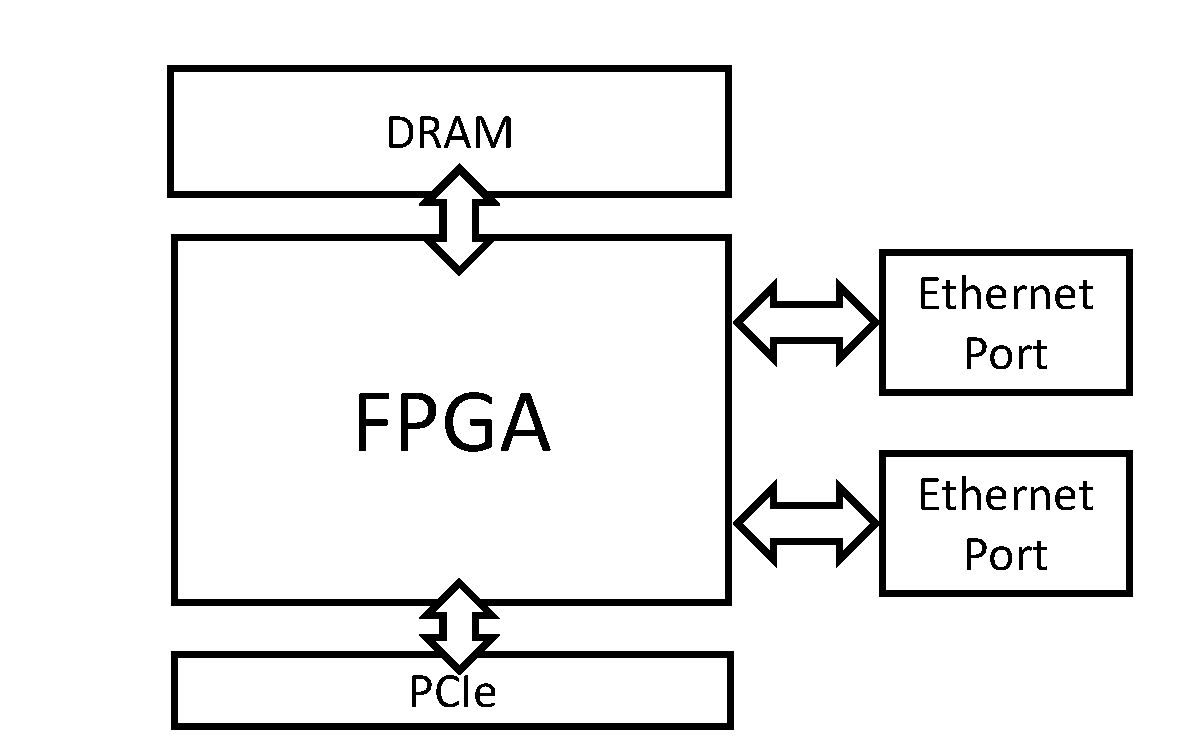
\includegraphics[width=0.6\textwidth]{fpga-board.pdf}
	
	\caption{FPGA板的逻辑图。}
	\label{clicknp:fig:fpga}
	
\end{figure}


与CPU或GPU相比,FPGA通常具有更低的时钟频率和更小的存储器带宽。
例如,FPGA的典型时钟频率约为200MHz,比CPU慢一个数量级(2至3~GHz)。
同样,FPGA的单块存储器或外部DRAM的带宽通常为2至10~GBps,而内存带宽约为Intel XEON CPU的40~GBps,GPU为100~GBps。
但是,CPU或GPU只有有限的内核,这限制了并行性。 FPGA内置了大量的并行性。
现代FPGA可能拥有数百万个LE,数百个K位寄存器,数十个M位BRAM和数千个DSP模块。从理论上讲,它们中的每一个都可以并行工作。
因此,FPGA芯片内部可能会同时运行数千个并行的``\textit {核}''。
虽然单个BRAM的带宽可能有限,但如果我们并行访问数千个BRAM,则总内存带宽可以是多TBps!
因此,为了实现高性能,程序员必须充分利用这种大规模的并行性。

传统上,FPGA使用诸如Verilog和VHDL之类的HDL进行编程。
这些语言水平太低,难以学习,编程也很复杂。
因此,大型软件程序员社区已经远离FPGA多年了~\cite {bacon2013fpga}。
为了简化这一点,许多高级综合(HLS)工具/系统已经在工业界和学术界开发,试图将高级语言(主要是C)的程序转换为HDL。
但是,正如我们将在第 \ref{chapter:clicknp} 章中看到的,它们都不适合网络功能处理,这是本工作的重点。


\subsection{架构对比}
\label{smartnic-comparison}

性能逐渐降低,可编程性逐渐提高。

如何选择,考虑几个方面:

\section{可编程网卡在数据中心的应用}
\label{background:sec:application}


\subsection{微软 Azure 云}

\begin{figure}[htbp]
	\centering
	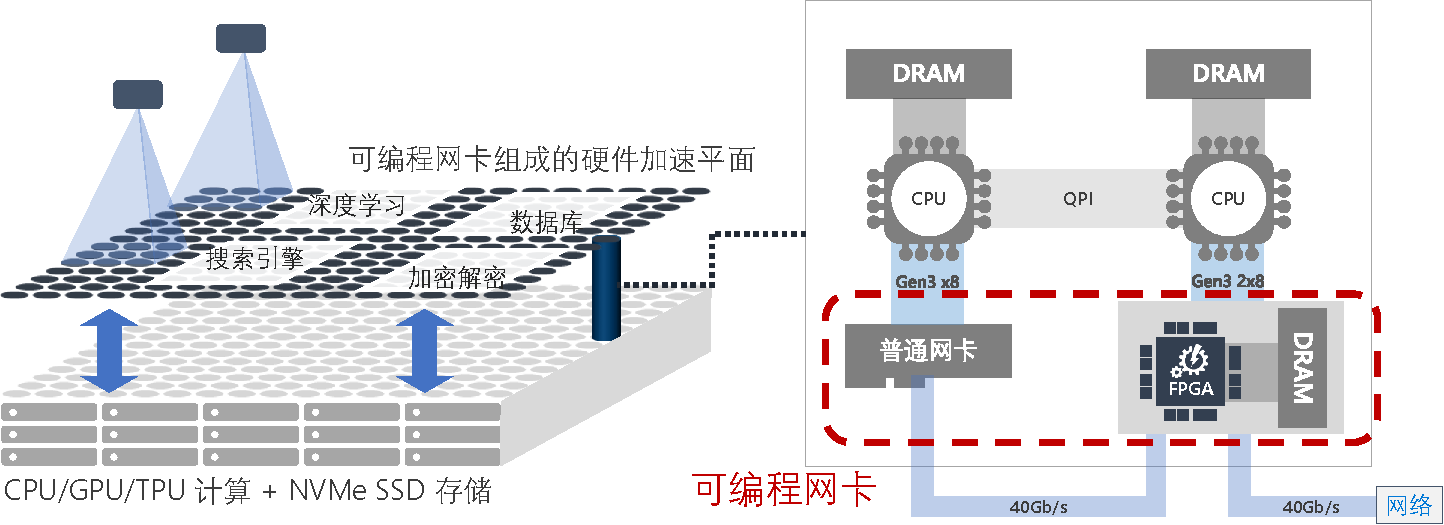
\includegraphics[width=0.8\textwidth]{figures/azure_fpga.pdf}
	\caption{微软基于 FPGA 的可编程网卡。}
	\label{background:fig:azure_fpga}
\end{figure}


New content:

1. CPU - accelerator communication
1) coherent memory
2) I/O DMA
3) Network

2. connectivity among accelerators
1) single server
2) rack
3) data center

3. device
1) FPGA
2) GPU
3) ASIC

New workloads:

compute offload

1) bing: hardware microservice, consolidation

2) compression and encryption: Office 365, Cosmos/Azure data lake, Onedrive

3) AI inference: neural networks, traditional models, AAAI'18

4) 3rd party: general computing acceleration device

infrastructure offload: (pioneer the wave of SmartNICs)

1) networking: network virtualization (compute node); NFV (network node)

2) persistent storage: SOSP'11; compression and encryption (backend): improve throughput; improve compression ratio, save storage space.
hypervisor and sharing (frontend)



微软对于把 FPGA 部署在哪里这个问题,大致经历了三个阶段:
\begin{enumerate}
	\item 专用的 FPGA 集群,里面插满了 FPGA;
	\item 每台机器一块 FPGA,采用专用网络连接;
	\item 每台机器一块 FPGA,位于网卡和交换机之间,共享服务器网络。
\end{enumerate}

第一个阶段是专用集群,里面插满了 FPGA 加速卡,就像是一个 FPGA 组成的超级计算机。像超级计算机一样的部署方式有几个问题:

\begin{enumerate}
	\item 不同机器的 FPGA 之间无法通信,FPGA 所能处理问题的规模受限于单台服务器上 FPGA 的数量;
	\item 数据中心里的其他机器要把任务集中发到这个加速机柜,构成了 in-cast 的网络流量特征,网络延迟很难做到稳定;
	\item FPGA 专用机柜构成了单点故障;
	\item 装 FPGA 的服务器是定制的,散热设计和运维都增加了复杂性。
\end{enumerate}

一种不那么激进的方式是,在每个机柜一面部署一台装满 FPGA 的服务器。这避免了上述问题 (2)(3),但(1)(4) 仍然没有解决。

第二个阶段,为了保证数据中心中服务器的同构性(这也是不用 ASIC 的一个重要原因),在每台服务器上插一块FPGA,FPGA 之间通过专用网络连接。这也是微软在 ISCA’14 上所发表论文采用的部署方式。

FPGA 采用Stratix V D5,有172K个ALM,2014个M20K片上内存,1590个 DSP。板上有一个8GB DDR3-1333 内存,一个PCIe Gen3 x8接口,两个10 Gbps网络接口。一个机柜之间的FPGA采用专用网络连接,一组10G网口8个一组连成环,另一组10G网口6个一组连成环,不使用交换机。

这样一个 1632 台服务器、1632 块 FPGA 的集群,把必应的搜索结果排序整体性能提高到了 2倍(换言之,节省了一半的服务器)。本地和远程的 FPGA 均可以降低搜索延迟,远程 FPGA的通信延迟相比搜索延迟可忽略。[4]

FPGA 在必应的部署取得了成功,Catapult 项目继续在公司内扩张。微软内部拥有最多服务器的,就是云计算 Azure 部门了。Azure 部门急需解决的问题是网络和存储虚拟化带来的开销。Azure把虚拟机卖给客户,需要给虚拟机的网络提供防火墙、负载均衡、隧道、NAT等网络功能。由于云存储的物理存储跟计算节点是分离的,需要把数据从存储节点通过网络搬运过来,还要进行压缩和加密。

为了加速网络功能和存储虚拟化,微软把 FPGA 部署在网卡和交换机之间。一块 FPGA(加上板上内存和网络接口等)的功耗大约是30 W,仅增加了整个服务器功耗的十分之一。只要规模足够大,对FPGA价格过高的担心将是不必要的。每个 FPGA 有一个 4GB DDR3-1333 DRAM,通过两个 PCIe Gen3 x8 接口连接到一个 CPU socket(物理上是 PCIe Gen3 x16 接口,因为 FPGA 没有 x16 的硬核,逻辑上当成两个 x8 的用)。物理网卡(NIC)就是普通的 40 Gbps 网卡,仅用于宿主机与网络之间的通信。


\textbf{图:微软SmartNIC可编程网卡的架构,其中FPGA位于网络和经典网卡之间}

FPGA(SmartNIC)对每个虚拟机虚拟出一块网卡,虚拟机通过 SR-IOV直接访问这块虚拟网卡。原本在虚拟交换机里面的数据平面功能被移到了 FPGA 里面,虚拟机收发网络数据包均不需要 CPU参与,也不需要经过物理网卡(NIC)。这样不仅节约了可用于出售的 CPU 资源,还提高了虚拟机的网络性能(25 Gbps),把同数据中心虚拟机之间的网络延迟降低了 10 倍。

这就是微软部署 FPGA 的第三代架构,也是目前「每台服务器一块 FPGA」大规模部署所采用的架构。FPGA 复用主机网络的初心是加速网络和存储,更深远的影响则是把 FPGA 之间的网络连接扩展到了整个数据中心的规模,做成真正 cloud-scale 的「超级计算机」。第二代架构里面,FPGA 之间的网络连接局限于同一个机架以内,FPGA之间专网互连的方式很难扩大规模,通过 CPU 来转发则开销太高。

第三代架构中,FPGA 之间通过 LTL (Lightweight Transport Layer) 通信。同一机架内延迟在 3微秒以内;8 微秒以内可达 1000 块 FPGA;20 微秒可达同一数据中心的所有 FPGA。第二代架构尽管 8台机器以内的延迟更低,但只能通过网络访问 48 块 FPGA。为了支持大范围的 FPGA 间通信,第三代架构中的 LTL 还支持PFC 流控协议和 DCQCN 拥塞控制协议。

通过高带宽、低延迟的网络互连的 FPGA构成了介于网络交换层和传统服务器软件之间的数据中心加速平面。除了每台提供云服务的服务器都需要的网络和存储虚拟化加速,FPGA上的剩余资源还可以用来加速必应搜索、深度神经网络(DNN)等计算任务。

对很多类型的应用,随着分布式 FPGA 加速器的规模扩大,其性能提升是超线性的。例如 CNN inference,当只用一块 FPGA 的时候,由于片上内存不足以放下整个模型,需要不断访问 DRAM 中的模型权重,性能瓶颈在DRAM;如果 FPGA 的数量足够多,每块 FPGA 负责模型中的一层或者一层中的若干个特征,使得模型权重完全载入片上内存,就消除了DRAM 的性能瓶颈,完全发挥出 FPGA 计算单元的性能。当然,拆得过细也会导致通信开销的增加。把任务拆分到分布式 FPGA集群的关键在于平衡计算和通信。

在 MICRO’16 会议上,微软提出了 Hardware as a Service(HaaS) 的概念,即把硬件作为一种可调度的云服务,使得 FPGA服务的集中调度、管理和大规模部署成为可能。


2016 年 9 月,《连线》(Wired)杂志发表了一篇《微软把未来押注在 FPGA 上》的报道 [3],讲述了 Catapult 项目的前世今生。紧接着,Catapult 项目的负责人 Doug Burger 在 Ignite 2016 大会上与微软 CEO Satya Nadella 一起做了 FPGA 加速机器翻译的演示。演示的总计算能力是 103 万 T ops,也就是 1.03 Exa-op,相当于 10 万块顶级 GPU 计算卡。



\subsection{亚马逊 AWS 云}

在 2017 年 12 月的 Re:Invent 大会上,亚马逊 AWS 云发布了名为 ``Nitro'' 的计算加速架构 \cite{nitro-blog}。
根据 2017 年 Re:Invent 大会和 2018 年 AWS 峰会上亚马逊发布的信息 \cite{nitro-talk,nitro-web},AWS 使用了定制 ASIC 来实现多种加速和安全功能。
最初,AWS 在 FPGA 和 ASIC 架构之间权衡,并决定采用 ASIC 方案。
为此,2015 年 1 月,亚马逊用 30 多亿美元收购了 ASIC 设计公司 Annapurna 实验室 \cite{annapurna},该公司以设计基于 ARM 核的片上系统(SoC)见长。

Nitro 项目的发展是分阶段的。与微软 Azure 类似,虚拟机的 I/O 瓶颈最早体现在虚拟网络上。早在 2013 年 11 月,AWS 的 C3 实例就引入了一块独立的网卡以实现高性能网络(enhanced networking),采用 SR-IOV 方式让虚拟机直接访问网卡,绕过虚拟机监控器中的虚拟交换机软件。此技术帮助 Netflix 实现了每秒 200 万个数据包的虚拟机网络吞吐量 \cite{netflix-aws}。

2015 年 1 月,AWS 的 C4 实例开始使用硬件加速弹性块存储(Elastic Block Storage,EBS)。弹性块存储的数据储存在存储节点上,而客户虚拟机运行在计算节点上,因此这是一种远程存储。对客户虚拟机而言,是一块虚拟存储设备,它是由虚拟机监控器 Xen Dom0 中的存储管理软件实现虚拟化的。C4 实例使用高性能网卡而非传统网卡来连接远程的弹性块存储,从而提高了性能。

2017 年 2 月,AWS 的 I3 实例引入了 NVMe 本地存储和专用的存储虚拟化芯片。以往,客户虚拟机访问本地存储,也需要经过虚拟机监控器中的存储管理软件,这是由于一台物理服务器中可能有多台虚拟机,每台虚拟机只能访问属于自己的那一部分存储空间,因此需要隔离。对延迟和吞吐量都很高的 NVMe 存储而言,存储虚拟化软件带来的开销太高了。为此,I3 实例引入的 Nitro 芯片在硬件上实现了存储隔离,因此可以通过 SR-IOV 把 NVMe 存储直通客户虚拟机,实现了每秒 300 万次 I/O 操作的存储性能 \cite{aws-local-storage}。

2017 年 11 月,AWS 的 C5 实例大幅改变了计算节点虚拟化的架构。首先,C4 实例中的远程存储仍然需要软件实现虚拟化,这一部分也可以像 I3 本地存储一样用硬件实现,不过块存储比本地存储的接口更复杂,因此硬件实现的难度更大。其次,在网络、远程和本地存储都已经使用硬件虚拟化后,事实上虚拟机监控器中的管理软件就只剩下数据平面的中断(APIC)功能和控制平面的管理功能了。控制平面的管理功能较为复杂,用纯数字逻辑显然是不现实的。为了把虚拟网络(VPC)、弹性块存储和虚拟化控制平面全部卸载(offload)到加速卡上,Nitro ASIC 采用了基于 ARM 核的片上系统架构,从而保持了数据平面的可编程性和灵活性,还能把控制平面一并卸载到加速卡上。

采用 Nitro 加速卡后,AWS 重新设计了一个轻量级的虚拟机监控器 Nitro 来取代 Xen,而原来运行在 Xen Dom0 上的控制平面转移到了 Nitro ASIC 里,客户虚拟机可以得到接近裸金属(bare-metal)主机的性能。此后,AWS 发布了裸金属实例,客户代码直接在物理机上运行,而所有的存储和网络资源都由 Nitro 卡提供。

Nitro 系列芯片主要包括三种芯片 \cite{nitro-blog,nitro-talk,nitro-web}:
\begin{enumerate}
	\item 云网络(VPC)和弹性块存储(EBS)加速芯片,一边连接数据中心网络,一边以 PCIe 卡的形式连接 CPU;
	\item 本地 NVMe 存储虚拟化芯片,作为 CPU 和 NVMe 存储设备之间的代理;
	\item 安全芯片,用于验证服务器中各种设备固件的版本,以及在裸金属服务器切换租户时重刷固件清除痕迹。
\end{enumerate}

Nitro 芯片的作用可以分为降低成本、提高性能和提高安全性三方面。下面详细讨论。

\textbf{节约 CPU 核。}
网络和存储虚拟化需要占用大量的 CPU 资源来处理每个网络包和存储 I/O 请求。
根据 ClickNP \cite{li2016clicknp} 估计,每个客户虚拟机的 CPU 核,需要预留另外 0.2 个 CPU 核来实现虚拟化。
如果这些功能可以被卸载到专用硬件,所节省的 CPU 核就可以用来安装客户虚拟机。
不管是考虑公有云虚拟机上每个 CPU 核的售价,还是考虑 Xeon CPU 每个核的硬件成本,用专用硬件都能获得明显的成本节约 \cite{smartnic}。

\textbf{提高最大核数。}
节约 CPU 核不仅能够降低成本,还能够提高大型虚拟机实例的最大核数。因为各大公有云厂商都从 Intel 等相同的厂商购买 CPU,因此同一时期能买到的最大 CPU 核数是相对固定的。虚拟化被卸载到硬件后,所有 CPU 核都用于运行客户虚拟机,因此 AWS 的 M5 实例最多可达 96 个 CPU 核。如果不使用硬件卸载,将只有 80 个 CPU 核可用于客户虚拟机,从而降低对追求极致性能客户的吸引力。

\textbf{提高单核频率。}
由于功耗墙的限制,CPU 的核心数目与平均核心频率不可兼得。同一代 CPU 架构下,较高核心频率的 CPU 核数一般较少。对于核数相等的虚拟机实例,如果使用传统的软件虚拟化,物理机就需要 1.2 倍的 CPU 核数,从而平均核心频率就可能降低。例如,在 C5 实例推出前的 72 核 EC2 实例,CPU 基频为 2.7 GHz,但采用同一代 Skylake 架构的 C5 实例虚拟机,CPU 基频就可以达到 3.0 GHz。

\textbf{提高本地存储性能。}
首先,在裸金属服务器上,本地 NVMe 存储可以达到每盘高达 400 K IOPS(I/O 操作每秒)的吞吐量。AWS I3 实例有 8 块 NVMe SSD,达到 3 M IOPS 的吞吐量。而对于常见的存储虚拟化协议栈,每个 CPU 核只能处理 100 K IOPS 左右的吞吐量,这意味着要占用 30 个 CPU 核才能让虚拟机充分利用 NVMe 存储的吞吐量,这个开销太高了。即使只有一块 NVMe 存储,4 个 CPU 核之间的负载均衡仍然是个难题 \cite{li2017kv}。如第 \ref{smartnic-architecture} 节所讨论的,由于硬件分配和处理任务是流水线式而非多个处理单元简单并行,硬件能够比多核软件更好地保证服务质量(QoS)。

其次,在延迟方面,裸金属服务器的 NVMe 存储平均延迟约为 80 微秒。虚拟化软件不仅会增加 20 微秒的平均延迟,而且由于操作系统调度、中断、缓存不命中等因素的影响,在高负载下的尾延迟(tail latency)可高达 1 毫秒(1000 微秒)。采用硬件卸载可以降低平均延迟 20\%,并降低高负载下的尾延迟 90\% 以上。

\textbf{提高远程存储性能和安全性。}
与本地存储类似,硬件加速可以提高远程存储性能。还有一点额外的优势:远程存储被公有云的所有租户共享,对可靠性和安全性要求更高。传统上远程存储协议在虚拟机监控器中运行,虽然逻辑上与客户虚拟机隔离,但由于共享 CPU、内存等资源,仍然不能排除零日(0-day)漏洞和边信道攻击的潜在安全隐患。把远程存储协议从主机 CPU 卸载到 Nitro 卡后,就有了更高的隔离性和更小的攻击表面(attack surface)。

\textbf{提高网络性能和安全性。}
在 Nitro 卡上实现网络虚拟化后,虚拟机可以直接通过 SR-IOV 访问网卡,达到数据中心网络 25 Gbps 的理论上限,尤其是对小数据包应用场景的性能提升明显。根据 ClickNP \cite{li2016clicknp} 估计,对 25 Gbps 线速(line-rate)的 64 字节小数据包,每秒高达 37 百万个,如果用软件虚拟交换机处理,将需要 60 个 CPU 核,这显然是不可接受的。因此大多数云服务商对虚拟网络(VPC)对吞吐量不仅有字节数的限制,还有数据包数的限制。大多数公有云的虚拟网络只支持数百万数据包每秒的吞吐量,需要处理大量小请求的远程过程调用(RPC)、键值存储(KVS)服务器就会遇到性能瓶颈。在延迟方面,软件虚拟化的 AWS 端到端延迟可达 100 微秒以上,而使用 Nitro 虚拟化加速后延迟就降低到 50 微秒以内了。硬件虚拟化对虚拟网络的尾延迟、服务质量和安全性的提升,也与远程存储相似。

\textbf{提高裸金属服务器安全性。}
最后,裸金属服务器上的客户代码可以直接访问服务器内的各种硬件设备,甚至可能烧写带外服务器管理(BMC)等组件的固件 \cite{bare-metal-security}。如果固件内被嵌入了恶意代码,并在下一个租户使用该裸金属服务器时被激活,后果不堪设想。事实上很大一部分客户选择裸金属服务器,正是出于对虚拟机隔离性的担忧。为了在租户开始使用裸金属服务器时提供安全和一致的硬件环境,Nitro 安全芯片会对固件进行重烧写。Nitro 还会在系统启动时进行完整性检查,这类似 UEFI 可信启动技术,但验证的范围不仅包括操作系统引导器,还包括硬件固件。

\subsection{阿里云、腾讯云、华为云}

2018 年,我国云计算服务商也积极地在数据中心部署了可编程网卡。阿里云和腾讯云部署可编程网卡的首要目的是支持裸金属(bare-metal)服务器。相比虚拟机,裸金属服务器可以消除虚拟化带来的开销,实现同样硬件条件下最高的性能;方便部署客户自己的虚拟化软件(如 VMWare);与客户在自有数据中心(on-premises)的部署环境完全相同,降低客户上云的迁移开销;方便使用不支持虚拟化或虚拟化后性能有较大损失的硬件,如 GPU 和 RDMA 网卡;不与其他租户共享服务器硬件,隔离性和安全性更强,也能符合一些客户的合规要求。

在公有云中使用裸金属服务器的主要技术挑战是访问数据中心内的虚拟网络(VPC)和远程存储(EBS)等资源。一种简单的方法是在同一个机架(rack)内放置若干虚拟网络和存储服务器,部署相应的软件;并在柜顶交换机(ToR switch)上配置转发规则,使裸金属服务器的所有网络数据包经过虚拟网络和存储服务器。这种方法需要增加额外的服务器资源,提高了成本。另一种方法是把虚拟网络和存储的数据平面卸载到柜顶交换机上。但是,柜顶交换机的编程灵活性一般较差 \cite{tencent-smartnic},不足以支持虚拟存储的应用层协议和虚拟网络的安全规则等。

因此,在服务器上增加一块可编程网卡便成为支持裸金属服务器性能最高的方案。阿里和腾讯采用了 FPGA 数据平面与多核 CPU 控制平面结合的 SoC 方案。2018 年,阿里云发布的 ``神龙'' 裸金属服务器使用自研的 MOC 卡 \cite{alicloud-smartnic,alicloud-xdragon} 实现类似 AWS Nitro 的网络、存储虚拟化。腾讯云在 APNet’18 上发布了基于 FPGA 的可编程网卡方案,主要用于网络虚拟化 \cite{tencent-smartnic}。腾讯仅用 10 个硬件工程师,就在三个月内完成了 FPGA 逻辑设计,用四个月做出了可编程网卡的板卡,并在一年内部署 \cite{tencent-smartnic}。这是 FPGA 编程也可以实现敏捷开发的例证。腾讯正在把可编程网卡的应用范围从裸金属服务器扩展到普通虚拟机,并对两种应用场景使用统一的可编程网卡架构。

华为基于海思半导体的技术积累,发布了两款可编程网卡,同时也用于华为云虚拟网络的加速。SD100 系列可编程网卡 \cite{sd100} 采用了基于多核 ARM64 CPU 的 SoC 架构,数据平面和控制平面都运行在 ARM CPU 上。IN5500 系列可编程网卡 \cite{in200} 采用网络处理器(NP)提供数据平面的可编程性,可达到 100 Gbps 性能。利用可编程网卡,华为云发布了 C3ne 网络增强虚拟机实例,在国内云厂商中率先实现了每秒千万级的数据包转发 \cite{huawei-smartnic}。

\section{架构概览}
\label{socksdirect:sec:architecture}




%As shown in Figure~\ref{socksdirect:fig:architecture}, the core component of \sys{} is a user-space library \libipc{}.

为了简化部署和开发 \cite {andromeda},以及消除内核交叉开销,本章在用户空间而不是内核中实现\sys{}。
要使用\sys{},应用程序通过设置\texttt {LD\_PRELOAD}环境变量来加载用户空间库\libipc {}。 \libipc {} 拦截标准C库(glibc)中与文件描述符操作相关的所有Linux API,在用户空间中实现套接字功能。
从安全的角度来看,因为\libipc {}驻留在应用程序地址空间中,它的行为不可信。例如,如果恶意应用程序在\libipc {}中强制执行,则可能会绕过防火墙策略。此外,如表 \ref{socksdirect:tab:socket-api} 所示,尽管大多数套接字操作可以在调用者本地或连接的两端之间实现,还有很多套接字操作需要中心化的协调。例如,TCP端口号是一个需要集中分配的全局资源 \cite {lin2016scalable,nsdi19freeflow}。因此,需要在\libipc {}之外的可信组件来强制实施访问控制和管理全局资源。

\begin{table*}[htbp]
	\centering
	\small
	\begin{tabular}{ll|ll}
		\toprule
		\multicolumn{2}{c|}{初始化} &
		\multicolumn{2}{c}{连接管理} \\
		\midrule
		API & 类别 &
		API & 类别 \\
		\midrule
		\textbf{socket} & Local &
		\textbf{connect} & NoPart \\

		bind & NoPart &
		\textbf{accept(4)} & P2P \\

		listen & NoPart &
		\textbf{\textit{fcntl, ioctl}} & Local \\

		socketpair & Local &
		\textbf{(get,set)sockopt} & Local \\

		getsockname  & Local &
		\textbf{\textit{close}, shutdown} & P2P \\

		\textbf{\textit{malloc}} & Local &
		getpeername & Local \\

		\textbf{\textit{realloc}} & Local &
		\textit{dup(2)} & P2P  \\

		\textit{epoll\_create} & Local &
		\textbf{\textit{epoll\_ctl}} & Local \\
		\bottomrule
		\toprule
		\multicolumn{2}{c|}{Data Transmission} &
		\multicolumn{2}{c}{Process Mgmt} \\
		\midrule
		API & 类别 &
		API & 类别 \\
		\midrule
		\textbf{recv(from,(m)msg)} & P2P &
		\textit{pthread\_create} & NoPart \\

		\textbf{\textit{write(v)}} & P2P &
		\textit{clone} & NoPart \\

		\textbf{\textit{read(v)}} & P2P &
		\textit{execve} & NoPart \\

		\textbf{\textit{memcpy}} & Local &
		\textit{exit} & P2P \\

		\textit{(p)select} & P2P &
		\textit{sleep} & P2P \\

		\textit{(p)poll} & P2P &
		\textit{daemon} & P2P \\

		\textbf{\textit{epoll\_(p)wait}} & P2P &
		\textit{sigaction} & Local \\
		\bottomrule
	\end{tabular}
	\caption{与套接字相关、被 \libipc{} 截获的主要 Linux API。分类包括本地(Local)、两端之间(P2P)和需集中协调、不可划分(NoPart)。\textit{斜体} 的 API 表示除了套接字,还有操作系统的其他用途。\textbf{粗体} 的 API 比其他 API 的调用更频繁,因此更值得优化。}
	\label{socksdirect:tab:socket-api}
\end{table*}



为此,本章在每个主机上设计一个\emph {monitor} 守护进程(下称 \textit{管程})来协调控制平面操作,例如连接创建。管程是系统服务。在每个主机中,所有加载\libipc {}的应用程序必须与主机的管程建立共享内存(共享内存)队列,从而形成控制平面。在数据平面上,应用程序构建对等队列以直接通信,从而减轻了管程守护程序的负担。图 \ref {socksdirect:fig:architecture} 显示了\sys {}的体系结构。


\begin{figure}[htbp]
	\centering
	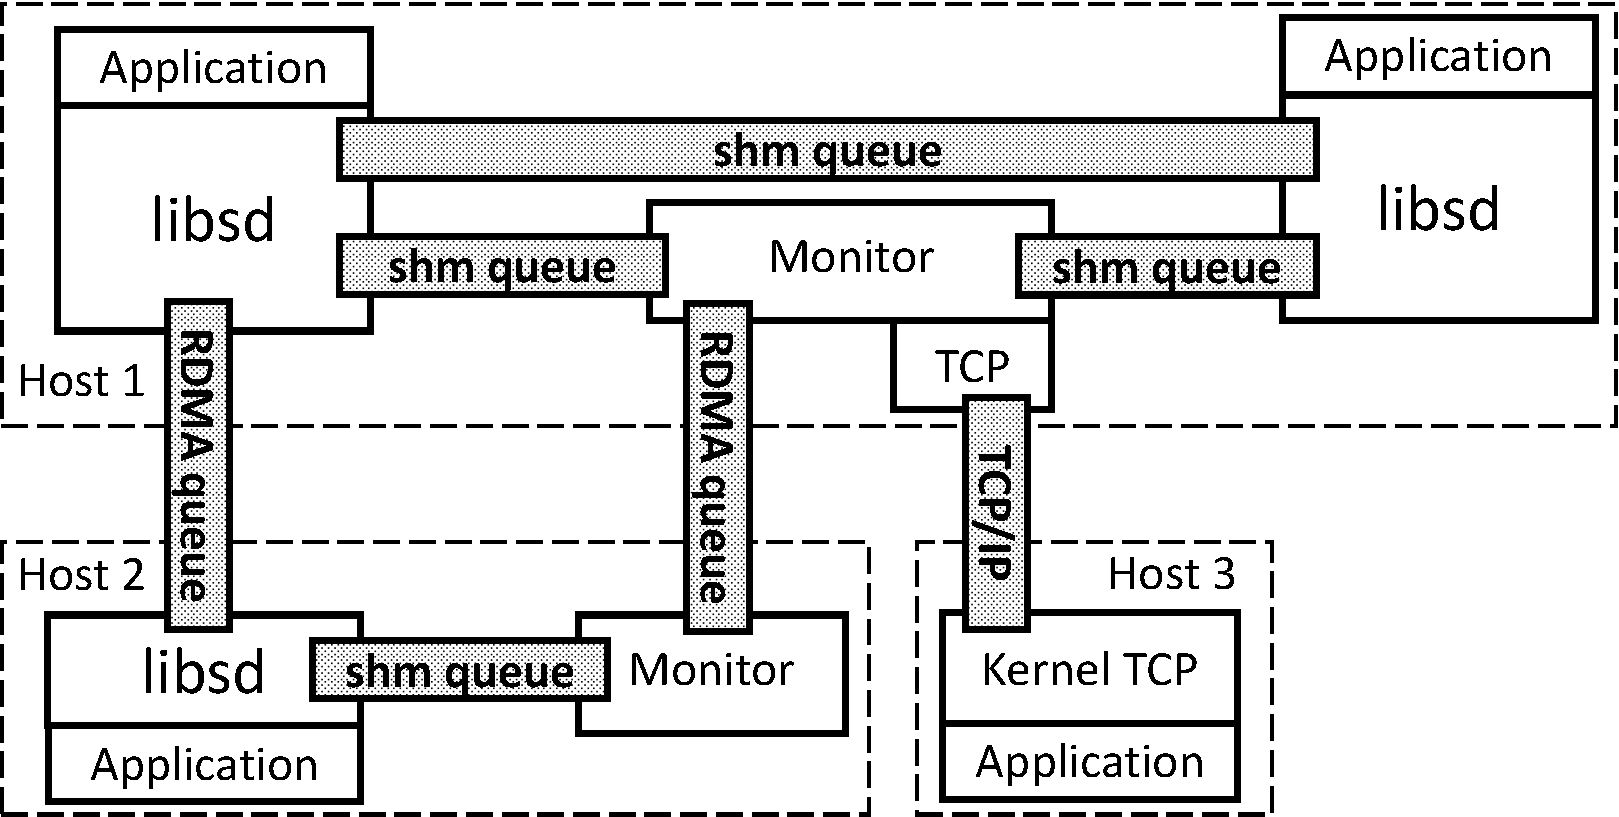
\includegraphics[width=0.8\textwidth]{images/architecture_new}
	\caption{\sys {}的体系结构。 主机1和2具有RDMA能力,而主机3不具备RDMA。}
	\label{socksdirect:fig:architecture}
\end{figure}


%To this end, we regard processes as a shared-nothing distributed system that communicates through message passing.
%We design a secure control-plane protocol between applications and the monitor, and a data-plane protocol between applications.

为了实现低延迟和高吞吐量,\sys {}使用共享内存进行主机内部和RDMA进行主机间通信。
每个套接字连接都映射到共享内存队列或RDMA QP。
共享内存或RDMA QP由唯一令牌标记,因此其他非特权进程无法访问它。
套接字发送操作转换为对远程端点上的套接字缓冲区的共享内存或RDMA写操作。

对于\emph {主机内}(intra-host)通信,通信发起者首先向本地管程发送请求,然后管程在两个应用程序之间(可能在不同的容器中)建立共享内存队列。 之后这两个应用程序可以直接通信。


%During initialization, \libipc{} connects to the local monitor via a shared memory queue.
%To enforce access control policies and support overlay networks, % and load balance new connections to multiple listeners, 
%connection request is always sent to the local monitor.
%For local peers, the monitor just construct a shared memory queue between the two applications , %so they can communicate directly.

对于\emph {主机间}(inter-host)通信,两个主机的管程都参与其中。当应用程序连接到远程主机时,其本地管程会建立常规TCP连接,并检测远程主机是否支持\sys {}。
如果是这样,它会在两个管程之间建立一个RDMA队列,以便可以更快地创建两个主机之间的未来连接。远程端的管程调度与目标的连接,并帮助两个应用程序建立RDMA队列,如图 \ref {socksdirect:fig:architecture} 中的主机1和2之间。如果远程主机不支持\sys {},它将继续使用TCP连接,如图 \ref {socksdirect:fig:architecture} 中的主机1和3之间。详细的连接管理协议在第 \ref {socksdirect:subsec:connection-management} 节中介绍。

为了确保线程安全并避免锁,以及支持fork和容器热迁移,本章针对只有一对发送和接收线程处于活动状态的常见情况进行了优化,同时确保所有情况下的正确性(第 \ref {socksdirect:subsec:fork} 节)。
为了消除缓冲区管理开销,设计了一个环形缓冲区,每个主机间消息平摊下来只需要一次RDMA写操作,每个主机内消息需要一个缓存迁移(第 \ref {socksdirect:subsec:lockless-queue}  节)。
本章进一步设计了一种零拷贝机制,可以在发送和接收端消除较大消息的数据拷贝(第 \ref {socksdirect:subsec:zerocopy} 节)。
最后,第 \ref {socksdirect:subsec:process-mux} 节提供了事件通知机制。


如图 \ref{socksdirect:fig:libsd-architecture} 所示,\libipc{} 运行库由 API 封装、虚拟文件系统(VFS)、队列、传输等四层构成。API 封装层使用 \emph {文件描述符重映射表} 来区分套接字文件描述符与内核文件描述符(例如文件和设备),在用户空间中实现套接字功能,并将其他系统调用通过标准 C 库(glibc)转发到内核。虚拟文件系统层实现了连接创建与关闭、事件轮询与通知、多进程共享套接字、fork、容器迁移等功能,是最复杂的一层。虚拟文件系统的旁边是信号层,负责接收来自操作系统的事件以及与管程、对端通信。下面一层是基于环形缓冲区的无锁队列。最下层是传输层,用共享内存(SHM)或 RDMA 实现。

\begin{figure}[htbp]
	\centering
	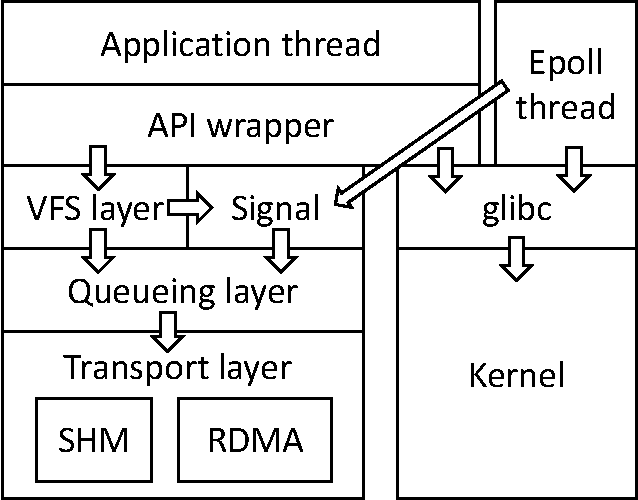
\includegraphics[width=0.5\textwidth]{images/libsd_architecture}
	\caption{\libipc{} 运行库的架构。}
	\label{socksdirect:fig:libsd-architecture}
\end{figure}


%In order to remove synchronization overhead for multi-threaded applications, we treat each thread as a separate process.
%%Although threads in a process share memory, we use thread-specific storage for most states in \libipc{}.
%For two communicating applications, we create peer-to-peer queues between each pair of sender and receiver threads to avoid synchronization cost of contending on the same queue.
%In Sec.~\ref{socksdirect:subsec:fork}, we present the peer-to-peer queue design that preserves FIFO ordering semantics and avoids starvation, especially when a process forks or creates a new thread.
%To maintain performance with many concurrent connections, rather than creating separate queues for each connection, we multiplex data from all connections through one queue.
%In Sec.~\ref{socksdirect:subsec:multiplex-conn}, we present the design of multiplexed queue that avoids head-of-line blocking and supports fetching data from any multiplexed connections.

%Inspired by Unikernels~\cite{madhavapeddy2013unikernels}, we move networking and IPC functions from the kernel to user space. Similar to existing works~\cite{peter2016arrakis,jeong2014mtcp,libvma}, we leverage multiple queues in modern 网卡s to enable user-space direct access to network. %The kernel is still responsible for process creation, scheduling, virtual memory and device management, but no longer on the critical path of performance.
%To maintain compatibility with existing Linux applications, we design a user-mode library \libipc as a drop-in replacement of the system call wrappers in the GNU C library (glibc). \libipc{} implements network socket functions in user mode, and adds a wrapper to other system calls to track process creation and memory allocation. \libipc{} is not considered a secure domain, as it shares memory space with the application. When \libipc{} is loaded, it creates a Linux native \textit{bootstrap socket} to the \textit{monitor} daemon, then creates a shared memory queue to the monitor.

%Even though multiple threads in the same process share memory space, we still treat each thread as a separated process and use thread-specific storage to store states in \libipc. In the following text, unless explicitly mentioned, we use a ``process'' to refer to a regular process or a thread.

\section{设计}
\label{socksdirect:sec:design}


\subsection{无锁套接字共享}
\label{socksdirect:subsec:fork}


大多数套接字系统为每个文件描述符维护一个锁,以使线程和进程共享套接字。
以前的工作 \cite {boyd2010analysis,clements2015scalable} 表明,许多套接字操作不可交换,并且不能始终避免同步。
本章利用共享内存消息传递比锁 \cite {roghanchi2017ffwd} 便宜得多的事实,并使用消息传递作为唯一的同步机制。


逻辑上,套接字由两个相反传输方向的FIFO \emph {队列}组成,每个FIFO具有多个并发的发送方和接收方。
系统设计目标是在保持FIFO语义的同时最大化通用情况性能。
本文观察到应用程序的如下两个特征:首先,由于成本高,高性能应用程序很少fork和创建线程。
其次,几个进程并发从共享套接字发送或接收并不常见,因为套接字的字节流语义使得很难避免接收部分消息。
需要同时发送或接收的应用程序通常使用消息代理(message broker) \cite {hintjens2013zeromq,rabbitmq2017rabbitmq,kreps2011kafka} 而非直接共享套接字。
常见的进程间套接字共享情况是应用程序隐式地将套接字从一个进程迁移到另一个进程,例如将事务从主进程卸载到工作进程。






\iffalse
Based on the observations, we propose the following requirements:

\begin{enumerate}[noitemsep,nolistsep]
 \item \textbf{Synchronization-free.} With multiple senders and receivers, if only one pair of sender and receiver is active, no synchronization should occur.
 \item \textbf{Multi-sender scalability.} Multiple processes may send data concurrently through a shared socket. With multiple active senders and a single receiver, if the receiver is not a bottleneck, the throughput should scale.
 \item \textbf{Self-stabilization.} Certain operations (\textit{e.g.} \texttt{fork}) may slow down the system temporarily, but after that the performance should converge back to normal.
\end{enumerate}

For compatibility with Linux semantics, we also need to ensure message ordering and liveness:
\begin{enumerate}[noitemsep,nolistsep]
\item \textbf{Single receiver ordering.} For a specific pair of sender and receiver, the received messages have the same ordering as they were sent.
\item \textbf{Multiple receiver ordering.} The order of \texttt{send} and \texttt{recv} operations for one sender and multiple receivers should be linearizable. If receiver $R_1$ receives $D_1$ before receiver $R_2$ calls \texttt{recv} and gets $D_2$, we guarantee that $D_1$ is sent before $D_2$.
\item \textbf{Deadlock-free.} If a socket buffer is not empty when \texttt{recv} is called by one or more receivers, at least one receiver should get data.
\item \textbf{Starvation-free.} If a sender keeps sending, any receiver trying to \texttt{recv} will eventually get some data.
\end{enumerate}
\fi

本章的解决方案是每个 \emph {套接字队列}(套接字的一个传输方向)有一个 \emph {发送令牌} 和一个 \emph {接收令牌}。
每个令牌都由一个 \emph {活跃线程} 持有,它具有发送或接收的权限。
因此,在任何时间点只有一个活动的发送方线程和一个活动的接收方线程。
套接字队列在线程和进程之间共享,允许来自一个发送方和一个接收方的无锁访问(详细信息将在第 \ref {socksdirect:subsec:lockless-queue} 节中讨论)。
当另一个线程想要发送或接收时,它应该请求 \emph {接管}(take over)令牌。



\begin{figure}[htbp]
	\centering
	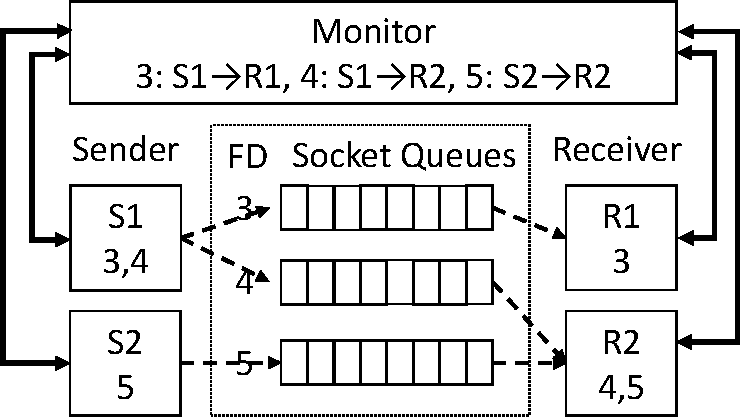
\includegraphics[width=0.6\textwidth]{images/queue_arch}
	\caption{无锁套接字与两个发送器和两个接收器线程共享。 虚线箭头表示每个套接字的活动发送方和接收方。 每个线程跟踪其活动套接字并通过独占队列与管程通信。}
	\label{socksdirect:fig:queue-arch}
\end{figure}


%\RED{Need performance comparison in a figure.}

每种类型的操作的详细信息如下:a)数据传输(\texttt {send}和\texttt {recv}),b)添加新的发送方和接收方(\texttt {fork}和线程创建 ),c)容器热迁移,和d)连接关闭。

\subsubsection{发送/接收操作}
\label{socksdirect:subsubsec:fork_rdwr}

\iffalse
\begin{figure}[htbp]
	\centering
	\subfloat[传统加锁。]{
		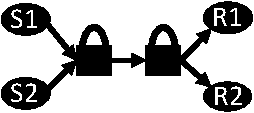
\includegraphics[width=0.3\textwidth]{images/one_conn3}
		\label{socksdirect:fig:fork-locking}
	}
	\hspace{0.02\textwidth}
	\subfloat[\sys{} 每个发送端一个。]{
		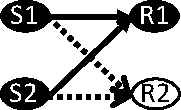
\includegraphics[width=0.22\textwidth]{images/one_conn1}
		\label{socksdirect:fig:fork-p2p}
	}
	\hspace{0.02\textwidth}
	\subfloat[S2 fork 成为 S2' 和 S3]{
		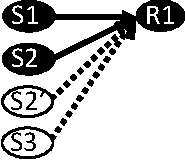
\includegraphics[width=0.2\textwidth]{images/one_conn2}
		\label{socksdirect:fig:fork-fork}
	}
	\caption{共享套接字的进程间队列结构。虚线箭头代表没有被启用的队列。}
	\label{socksdirect:fig:inter-process-queue}
\end{figure}
\fi


当一个线程没有发送令牌但想要通过套接字发送时,非活动线程需要\emph {接管}令牌。
如果在非活动线程和活动线程之间创建直接通信通道,则需要点对点的队列,其数量为线程数的平方,或者是具有锁的共享队列。
为了避免这两种开销,在\emph {接管}过程中使用监控守护进程作为代理。
此消息传递设计还具有以下优点:发送方进程可以位于不同的主机上,这在容器热迁移中非常有用。

接管过程如下:
非活动发送方向管程发送\emph {接管}命令,管程将其添加到等待列表并将命令代理到活动发送方。
当活动发送方收到请求时,它会将发送令牌发送给管程。
管程将令牌授予等待列表中的第一个非活动发送方,并更新活动发送方。
非活动发送方可以在收到令牌后发送。
此机制无死锁,因为至少有一个发送方或管程持有发送令牌。
它也是无饥饿的,因为每个发送方最多可以出现在等待列表中一次,并按FIFO顺序提供。

接收器侧的接管过程类似。


%\begin{figure}[t]
%	\centering
%	
\includegraphics[width=0.3\textwidth]{images/fixme}
%	\caption{This figure shows a stable connection handled by multiple senders and receivers.}
%	\label{socksdirect:fig:fork-bipartitegraph}
%\end{figure}

\subsubsection{Fork,Exec 和线程创建}
\label{socksdirect:subsubsec:fork_fork}


\textbf {套接字数据共享。}
主要的挑战是在\texttt {fork}和\texttt {exec}之后共享套接字元数据、缓冲区和底层的传输层。
在fork之后,内存空间变为写时复制,并在exec之后被擦除,但是套接字文件描述符仍需要可用。
\sys{} 使用共享内存(共享内存)来存储套接字元数据和缓冲区,因此在fork之后,数据仍然是共享的。
要在exec之后附加共享内存,\libipc {}将连接到管程以获取其父进程的共享内存密钥。
在fork之后,因为父进程看不到子进程创建的套接字,所以子进程创建一个新的共享内存来存储新套接字的元数据和缓冲区。

现在需要共享连接到对等端的底层传输。
共享内存传输不需要特别小心,因为fork / exec之前创建的共享内存仍然在fork / exec之后共享。
但是,RDMA在fork / exec后存在问题,因为DMA内存区域不在共享内存中。
它们在fork之后变为写时复制,而网卡仍然从原始物理页面DMA,因此子进程不能使用现有的RDMA资源。
而在exec之后,整个RDMA上下文将被清除。
本章的解决方案是让子进程在fork / exec之后重新初始化RDMA资源(PD,MR等)。
当子进程使用在fork之前创建的套接字时,它会要求管程与远程端点重新建立RDMA QP。
因此,对端进程可能会看到一个套接字的两个或更多QP,但它们链接到套接字元数据和缓冲区的唯一拷贝。
图 \ref {socksdirect:fig:fork-memory} 显示了一个fork示例。


\begin{figure}[htbp]
	\centering
	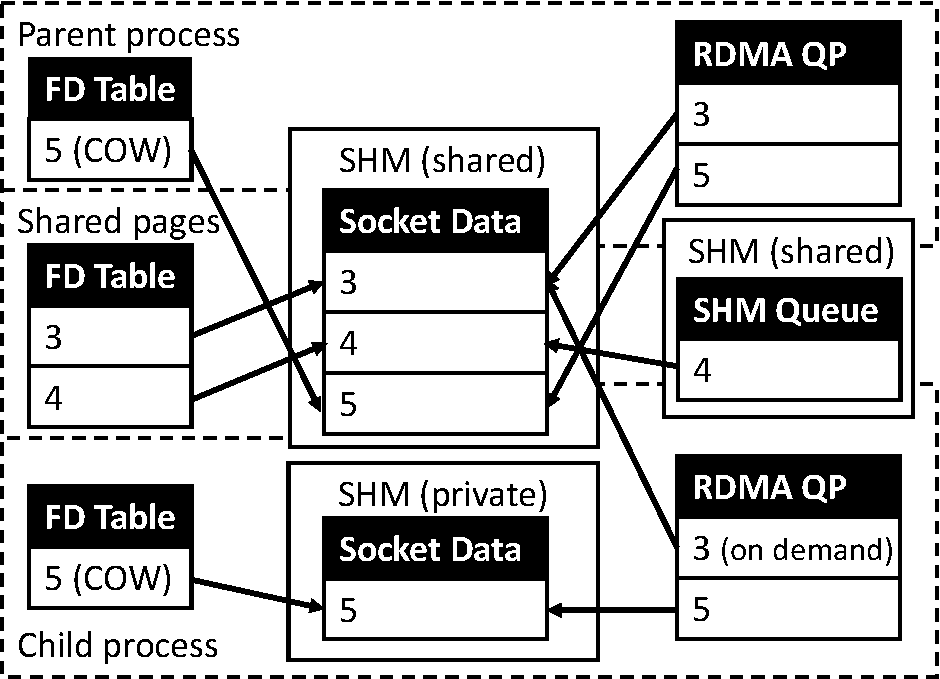
\includegraphics[width=0.6\textwidth]{images/fork_memory}
	\caption{fork后的内存布局。 文件描述符 3和4在fork之前创建并因此共享。 在fork之后,父进程和子进程分别创建一个新的文件描述符 5,它在文件描述符表中写入时被复制。 文件描述符 3和4的套接字元数据和缓冲区在共享内存中并因此被共享。 子进程创建一个新的共享内存来存储文件描述符 5的套接字元数据和缓冲区,当它再次fork时,它将与子进程共享。 RDMA QP位于私有内存中,而共享内存队列是共享的。}
	\label{socksdirect:fig:fork-memory}
\end{figure}


\textbf {文件描述符空间共享。}
与套接字数据不同,文件描述符空间在fork之后变为写时复制:fork 前创建的文件描述符是共享的,但新文件描述符由创建者进程独享。
因此,只需将文件描述符重映射表驻留在堆内存(heap memory)中,利用 fork 之后操作系统的写时复制机制。
要在exec之后恢复文件描述符重映射表,它将在exec之前复制到共享内存,并在\libipc {}初始化期间拷贝回新进程。

\textbf{安全。}
安全性是一个问题,因为恶意进程可能将自己伪装成特权父进程的子进程。
要在管程中标识父关系和子关系,当应用程序调用\texttt {fork},\texttt {clone}或\texttt {pthread\_create}时,\libipc {}首先生成一个用于配对的密钥并将其发送到管程,然后调用\emph {libc}中的原始函数。
在fork之后,子进程为管程创建一个新的共享内存队列并发送密钥(子进程继承父内存空间,从而知道该密钥)。
因此,管程可以将子进程与父进程配对。

\textbf {管程操作。}
在fork,exec或线程创建时,管程需要新进程添加到每个现有套接字的发送方和接收方列表中,以便管理接管操作。

%The socket queues are in 共享内存 between parent and child processes.
%However, to avoid synchronization in accessing shared metadata, the metadata is in thread local storage and copied from parent to child.
%To maintain isolation between parent and child, monitor creates new shared memory queues to replace all queues in \emph{both} parent and child, as Figure~\ref{socksdirect:fig:fork-fork} shows. We do not reuse queues due to potential isolation violation. %The monitor then sends credentials of new queues to parent and child via bootstrap sockets. 
%Each peer process is notified of the new queues and the new process. From then on, parent and child processes have isolated queues to the monitor and peers.

%A harder challenge comes from socket connection sharing between parent and child processes.
%A major challenge is how to handle the remaining data in the original send and receive queues.

%For each unidirectional queue, we discuss the behavior of related processes in four cases:
%\begin{enumerate}
%	\item A sender process itself forks.
%	\item A receiver of a sender process forks.
%	\item A receiver process itself forks.
%	\item A sender of a receiver process forks.
%\end{enumerate}

%The general process of fork is that after monitor is notified of the fork, it creates shared memory between the newly created process and all the processes which previously have connections with the parent process. The key challenge lies in the fork is that how to deal with the existing data in the connection to guarantee the order requirements.

%\textbf{Receiver fork.}
%First we look at a simple case when a receiver forks. Recall that only one receiver has exclusive access to a socket, as stated in Sec.~\ref{socksdirect:subsubsec:fork_rdwr}. The parent process inherits receive permission. When a sender receives fork notification of its peer, it copies all data from original queues to new queues of the parent process.

%\textbf{Sender fork.}
%When a sender forks, things are more complicated. We need to guarantee that all data sent prior to \texttt{fork} is consumed before the data sent after \texttt{fork}.

%Our solution is to let receivers drain the original queue first before switching to the new queues. After \texttt{fork}, both parent and child send data to its new queue. When the receiver is notified of the fork, it keeps track of the original queue and consumes all data in it before activating new queues. Note that the parent or child may fork again before the original queue is drained. With this in mind, the receiver maintains a forest data structure to track dependency of queues. The root of each tree in the forest is the oldest queue to receive from. Each non-leaf node has two children indicating the new queue of parent and child processes. If a non-leaf root queue becomes empty, it will be removed, and the two children queues will be promoted to root nodes.

%\textbf{Takeover During Fork.}
%After a sender forks, the receivers still need the takeover mechanism to arbitrate remaining messages in the original queue. However, both parent and child senders have dropped the original queue and will not respond to takeover requests. A similar situation occurs when a sender process dies. Our solution is to let the receivers use atomic operations to compete for remaining data in the original queue. Since this case rarely happens, the performance of the overall design is not affected.

%Things become much more complicated when cases 1,4 happens after cases 2,3 happening. After receiver forks, the unique sender is responsible for receiving ``takeover message'' and resend the data to new receivers. However, if sender forks following the receiver forks, according to the methods we mentioned above, there is no sender responsible for processing ``takeover message''. Our solution is that we require the receivers to poll the data from the old shared memory queue and compete for data. Since this case rarely happens, the performance of the overall design is not affected.

\subsubsection{容器热迁移}
\label{socksdirect:subsubsec:container_live_migration}


\textbf {在套接字队列中迁移剩余数据。}
由于\libipc {}在与应用程序相同的进程中运行,因此其内存状态将与应用程序一起迁移到新主机。
内存状态包括套接字队列,因此不会丢失正在传输(已发送但未接收)的数据。
套接字只能在容器内共享,并且容器中的所有进程都会一起迁移,因此迁移后可以取消分配原始主机上的内存。

\textbf {监控状态的迁移。}
管程跟踪侦听套接字信息,活动线程和每个连接的等待列表以及共享内存密钥。
在迁移期间,旧管程会转储已迁移容器的状态并将它们发送到新管程。

\textbf {建立新的通信通道。}
迁移后,所有通信通道都已过时,因为共享内存在主机上是本地的,而RDMA不支持热迁移 \cite{nsdi19freeflow,slim}。
首先,新主机上的迁移容器需要与本地管程建立连接。
本地管程指示以下过程。
两个容器之间的主机内连接可能变为主机间,因此\libipc {}在这种情况下创建RDMA连接。
两个容器之间的主机间连接可能成为主机内部,\libipc {}创建共享内存连接。
最后,\libipc {}重新建立剩余的主机间RDMA和主机内共享内存连接。


%\subsubsection{Connection Creation}
%\label{socksdirect:subsubsec:fork_new}
%

%A connection created by a thread can be accessed by all threads in the same process.
%To avoid creating redundant queues and connection states, \libipc does not share the 文件描述符 eagerly with other threads, because most threads in existing applications do not use connections created by other threads.
%When a thread do want to accesses a 文件描述符 that belongs to another thread, \libipc sends a message to the owner thread and requests sharing the 文件描述符. %This procedure is exactly the same as sharing existing connections during thread creation (Sec.~\ref{socksdirect:subsubsec:fork_fork}). %The sharing procedure only happens once for every connection and thread. Sharing existing connections eagerly during thread creation is an optimization. First, children threads are more likely to use existing connections than siblings. Second, batch processing improves performance.

%\subsubsection{Connection Close}
%\label{socksdirect:subsubsec:fork_close}
%

%Close is the operation that all of the processes leave the connection. The synchronization is  especially challenging since all the processes are run in parallel. One challenge lies in file descriptors are managed by decentralized processes and are possibly reused. One process close a connection while the others are doing compute intensive tasks is a case. It is possible that the file descriptor of the old process is reused and a new connection is setup with the same file descriptor. The other process may notice the close of the old connection and also call close on its own side, which lead to the new connection setup by the previous process closed due to the match of same file descriptor. 

%To satisfy the synchronization requirements, the close function call is all completed by message passing. The caller of close need to wait for ACK from all the other peers before release resources. i.e. the status of the connection.

%\textbf{Broadcast.}
%When a process calls \texttt{close}, all its peers cannot send to or receive from the 文件描述符. In this sense, 
%A socket is closed if all shared processes close it. So, we need to multicast a notification to the peers and collect responses from them. A challenge arises when \texttt{close} is interleaved with \texttt{fork}. Since \texttt{fork} and \texttt{close} do not commute~\cite{clements2015scalable}, we need a rule to determine their partial order. We make the choice that the ordering is determined by the initiator of \texttt{close}. If a process calls \texttt{close} before receiving fork notification, it will piggyback close notification with fork completion to both parent and child processes.

%\textbf{Handshake before releasing resource.}
%Another challenge is caused by 文件描述符 reuse after close. As stated in Sec.~\ref{socksdirect:subsec:socket-api}, a 文件描述符 is deleted after receiving shutdown message of both directions. With multiple processes sharing a connection, after one process calls \texttt{close}, others can still use the connection. Consequently, a process deletes a 文件描述符 only after receiving shutdown messages of both directions from all peers of the 文件描述符.

%Another challenge lies in the close of a connection is that close is a broadcast operation while send/receive is sent to a specific process. Besides, fork and close are immutable operations while the scalability requirements of the system impose the constraint that all the operations run asynchronously. As a result, a rule to determine the partial order is required.

%In \libipc, we make the choice that the order of fork and close is determined at the start point of the fork operation and the end point (after receiving all the ACKs). By making this choice, when a process waiting fork close ACK encounters fork message, it could send a separate close request to newly created process, which guarantees all the processes closed.

\subsection{带RDMA和SHM的环形缓冲区}
\label{socksdirect:subsec:lockless-queue}

\iffalse
\begin{figure}[t]
	\centering
	
\includegraphics[width=0.4\textwidth]{images/fixme.pdf}
	
	\caption{队列的性能比较。}
	\label{socksdirect:fig:queue-performance}
\end{figure}
\fi

\begin{figure}[t]
	\centering
	\subfloat[传统环形缓冲区。]{
		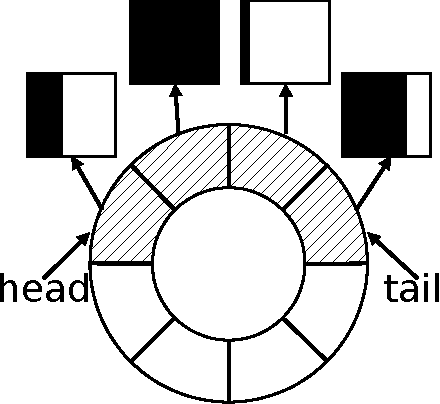
\includegraphics[width=0.3\textwidth]{images/ringbuffer_traditional}
		\label{socksdirect:fig:ringbuffer-traditional}
	}
	\hspace{0.02\textwidth}
	\subfloat[\sys.]{
		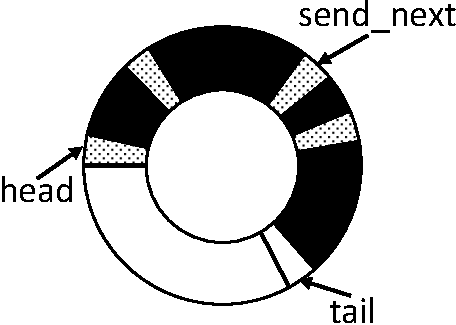
\includegraphics[width=0.32\textwidth]{images/ringbuffer_new}
		\label{socksdirect:fig:ringbuffer-new}
	}
	
	\caption{环缓冲数据结构。 阴影部分是包元数据,黑色部分是有效载荷。}
\end{figure}

传统上,网络堆栈使用环形缓冲区从网卡发送和接收数据包。
如图 \ref {socksdirect:fig:ringbuffer-traditional}所示,它会导致缓冲区管理开销和内部碎片。
传统的网卡支持有限数量的环形缓冲区,因此多个连接可以通过一个环形缓冲区进行复用,这种设计可以将有效负载移动到每个连接缓冲区而无需复制。
幸运的是,RDMA编写动词开辟了新的设计可能性。
本章的创新是拥有\emph {每个套接字连接一个环形缓冲区}并将数据包背靠背存储,如图 \ref {socksdirect:fig:ringbuffer-new}所示。
发送方确定环形缓冲区和偏移量(即\emph {tail}指针),然后使用RDMA写动词将数据包写入远程端内存中的尾指针。
在传输过程中,接收器CPU不需要做任何事情。
当接收器应用程序调用\texttt {recv}时,数据从\emph {head}指针中出列。
SHM的过程类似,因为SHM和RDMA都支持写原语。

要判断环形缓冲区是否已满,发送方将保持\textit {queue credits}计数,指示环形缓冲区中的空闲字节数。
当发件人将数据包入队时,它会消耗信用。 当接收器使消息出列时,它会在本地递增计数器,并在计数器超过环形缓冲区大小的一半时在发送者的内存中写入\textit {credit return flag}。 发送者在检测到标志时重新获得队列信用。
请注意,此机制与拥塞控制无关; 后者由网卡硬件处理 \cite {zhu2015congestion}。

\textbf {发送和接收方的两个环形缓冲区副本。}
上述机制仍然会在发送端引起缓冲区管理,因为发送方需要在缓冲区中构造RDMA消息。
其次,它不支持容器实时迁移,因为RDMA队列中的剩余数据很难迁移。
第三,本章的目标是批量处理小消息以提高吞吐量。
为此,本章在发送方和接收方都保留了环形缓冲区的副本。
发送方写入其本地环形缓冲区,并调用RDMA以使发送方与接收方同步。
\libipc{} 为每个环形缓冲区使用一个 RDMA RC QP,并维护一个机上RDMA消息的计数器。
如果计数器未超过阈值,则为每个socket \texttt {send}操作发送RDMA消息。
否则,不发送消息,\emph {send\_next}标记第一个未发送的消息。
完成RDMA写入后,\libipc{} 会在图 \ref {socksdirect:fig:ringbuffer-new}中发送包含所有未发送更改的消息(\emph {send\_next}到\emph {tail})。
这种自适应批处理机制可最大限度地减少空闲链路上的延迟,并最大化繁忙链路上的吞
对于SHM,只有一个由两个进程共享的环形缓冲区副本,并且同步由高速缓存一致性硬件完成。

%Before sending, sender clears header of the next message to prevent the receiver from considering junk data in the ring buffer to be a message. Next, sender writes payload, then writes header, finally advances \textit{tail}. Receiver polls \textit{isvalid} at \textit{head} pointer, then copies the message, finally advances \textit{head}.
%For RDMA, the sender maintains a local copy of ring buffer, and we use one-sided RDMA write to synchronize updates from sender to receiver.
%For RDMA, it is known that one-sided verbs has higher throughput than two-sided ones; short messages has lower throughput than large ones~\cite{kalia2014using,kaminsky2016design}.
%In light of this, the inter-host queue has two identical copies in pinned sender and receiver memory, and we use one-sided RDMA write to synchronize updates from sender to receiver.
%\libipc{} polls CQ to limit the number of in-flight (sent but not acknowledged) messages, which is not only required by RDMA 网卡, but also enables \emph{adapative batching}~\cite{li2016clicknp,li2017kv}.
%When a message is enqueued to the ring buffer and the RDMA send queue is not full, it is immediately sent as an RDMA message.
%When \libipc{} polls CQ and finds an empty slot in send queue, it sends all queued but unsent data in queue as an RDMA message, because the messages are stored back-to-back in the queue.


\textbf {有效载荷和元数据之间的一致性。}
对于SHM,英特尔和AMD的X86处理器提供了整体商店订购 \cite {sewell2010x86,intel-manual},这意味着其他内核按照与编写时相同的顺序观察到两次写入。一个8字节的\texttt {MOV}指令是原子的,所以写一个标题是原子的。由于发送方在有效负载之后写入标头,因此接收方将读取一致的消息因此,不需要存储器栅栏指令。

因为RDMA不能确保消息中的写入顺序 \cite {infiniband2000infiniband},确实需要确保消息完全到达。虽然在使用go-back-0或go-back-N loss recovery~ \cite {dragojevic2014farm}的RDMA网卡中观察到消息写入顺序,但对于具有选择性重传的更高级网卡,情况并非如此 \cite {mprdma,mittal2018revisiting} 。在\libipc {}中,发送方使用\textit {RDMA write with immediate}动词在接收方生成完成。接收器轮询RDMA \emph {完成队列}而不是环形缓冲区。 RDMA确保接收器上的高速缓存一致性,并且在将数据写入\libipc {}环形缓冲区 \cite {infiniband2000infiniband}之后保证完成消息。


\textbf {平摊轮询开销。}
当不经常使用套接字时,轮询环缓冲区会浪费接收器的CPU周期。本章使用两种技术分摊轮询开销。
首先,对于RDMA队列,利用RDMA 网卡将事件通知复用到单个队列中。
每个线程对所有RDMA QP使用\emph {共享完成队列},因此它只需要轮询一个队列而不是所有每个套接字队列。

其次,每个队列可以在\textit {polling}和\textit {interrupt}模式之间切换。监视器的队列始终处于轮询模式。每个队列的接收者维护一个连续空轮询的计数器。当它超过阈值时,接收器向发送器发送消息,通知队列正在进入中断模式,并在短时间后停止轮询。当发送方以中断模式写入队列时,它还会通知监视器,监视器将通知接收方恢复轮询。


%\RED{Need a performance comparison figure of ring buffer architectures. (traditional ring buffer, new ring buffer, intra, inter, x axis: msg size, y axis: throughput)}

\subsection{零拷贝}
\label{socksdirect:subsec:zerocopy}

\begin{figure}[t]
	\centering
	\subfloat[服务器内SHM。 1)获取物理页面并设置写入时复制; 2)通过SHM发送页面地址; 3)映射收到的页面; 4)(可选)在发送者写入/ memcpy / recv时重新映射。]{
		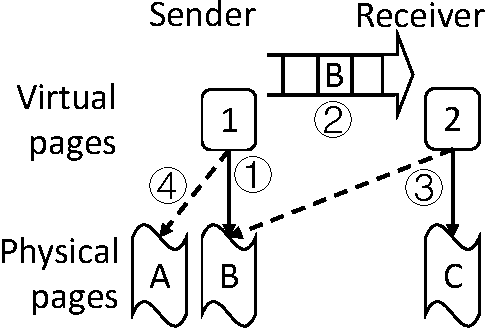
\includegraphics[width=0.44\textwidth]{images/zerocopy_intra}
		\label{socksdirect:fig:zerocopy-intra}
	}
	\hspace{0.02\textwidth}
	\subfloat[服务器间RDMA。 1)获取物理页面并设置写入时复制; 2)从池中获取免费页面; 3)通过RDMA发送数据; 4)通过RDMA发送页面地址; 5)地图收到的页面; 6)将未映射的页面返回到池。]{
		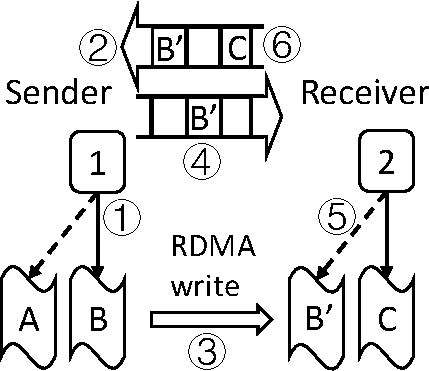
\includegraphics[width=0.42\textwidth]{images/zerocopy_inter}
		\label{socksdirect:fig:zerocopy-inter}
	}
	
	\caption{发送零拷贝页面的过程。}
\end{figure}


正如第 \ref {socksdirect:subsec:per-byte-overhead} 节所讨论的,零拷贝的主要挑战是维护套接字API的语义。
幸运的是,虚拟内存提供了一个间接层,许多相关工作利用了这种\emph {页面重映射}(page remapping)技术,从而可以将物理页面从发件人的虚拟地址重新映射到接收者,而不是复制。
Linux零复制套接字 \cite {linux-zero-copy}仅支持发送方,通过将数据页设置为写时复制。
但是,许多应用程序经常覆盖发送缓冲区,因此写时复制机制只是将复制从\texttt {send}时间延迟到第一次覆盖时间。
为了实现零拷贝接收,20年前,BSD~ \cite {thadani1995efficient}和Solaris~ \cite {chu1996zero}将应用缓冲区的虚拟页面重新映射到系统缓冲区的物理页面。但是,正如Table~ \ref {socksdirect:tab:operation-performance}所示,在现代CPU上,由于内核交叉和TLB刷新成本,映射一个页面的成本甚至比复制它更高。
最近,许多高性能TCP / IP堆栈 \cite {han2012megapipe,yasukata2016stackmap}和socket-to-RDMA库 \cite {rsockets,socketsdirect}提供标准套接字API和备用零拷贝API,但它们都没有实现标准API的零拷贝。
此外,没有现有的工作支持主机内套接字的零拷贝。



%A sender may write the send buffer after non-blocking \texttt{send}, and the receiver does not know the receive buffer before \texttt{recv}.
% so we can remap virtual address of a buffer to another physical page if the data occupies entire 4~KiB pages.


要启用零拷贝,需要修改网卡驱动程序以公开与页面重新映射相关的几个内核函数。
为了分摊页面重新映射成本,\libipc{} 仅对\texttt {send}或\texttt {recv}使用零拷贝,且有效载荷至少为16~KiB。
而是复制较小的消息。

\textbf {内存对齐。}
页面重新映射仅在发送和接收地址页面对齐且传输包含整个页面时才有效。
\libipc{} 拦截\texttt {malloc}和\texttt {realloc}函数,并为具有多个4K大小的分配分配4~KiB对齐的地址,因此大多数缓冲区将与页面边界对齐,而不会浪费内存用于小分配。
如果发送消息的大小不是4~KiB的倍数,则最后一块数据将复制到\texttt {send}和\texttt {recv}。

有时,应用程序需要并不从分配的缓冲区起始地址开始接收或发送数据。例如,数据为 HTTP 请求的一部分,HTTP 请求的内存是对齐的,而由于 HTTP 头的存在,数据就不是对齐的了。
对于非对齐情况,如果应用程序在接收之后直接发送,而没有读写数据本身,\sys{} 也可以实现零拷贝的消息传输。\sys{} 的方法是对于非对齐的接收缓冲区,默认不执行内存拷贝,而是记录页面的映射和偏移量关系。在应用程序首次访问时通过页面异常触发数据拷贝;如果应用程序不访问数据,则无需拷贝。

%\textbf{Amortize page remapping cost.}


\textbf{减少写时复制。}
当发送者在\texttt {send}之后覆盖缓冲区时,现有设计使用copy-on-write。
复制是必需的,因为发件人可能会读取页面的未写入部分。
由于应用程序几乎总是将缓冲区重用于后续发送操作,因此在大多数情况下会调用copy-on-write,这使得零拷贝在发送方上基本无用。
我们观察到,大多数应用程序不会逐字节写入发送缓冲区。 相反,它们会通过\texttt {recv}或\texttt {memcpy}覆盖发送缓冲区的整个页面,因此无需复制页面的原始数据。
对于\texttt {memcpy},\libipc{} 调用内核重新映射新页面并禁用copy-on-write,然后执行实际复制。
对于\texttt {recv},旧页面映射将被接收的页面替换。


\textbf {页面分配开销。}
页面重新映射需要内核为每个零拷贝\texttt {send}和\texttt {recv}分配和释放页面。
内核中的页面分配使用全局锁定,这是低效的。 \libipc {}在本地管理每个进程中的可用页面池。
\libipc {}还跟踪收到的零拷贝页面的来源。
当页面未映射时,如果它来自另一个进程,\libipc {}会通过消息将页面返回给所有者。

\textbf {通过SHM安全发送页面地址。}
对于主机内部套接字,在用户空间队列中的消息中发送物理页面地址,如图 \ref {socksdirect:fig:zerocopy-intra} 中的步骤2所示。
\sys{} 必须防止未经发送端允许的任意页面映射。
为此,\libipc {} 调用修改后的网卡驱动程序
获取发送缓冲区的模糊物理页面地址,并通过共享内存队列将地址发送给接收方。
在接收端,\libipc {} 调用内核将模糊的物理页面重新映射到应用程序提供的接收缓冲区虚拟地址。

\textbf {RDMA下的零拷贝。}
\libipc {}初始化接收器上的固定页面池,并将页面的物理地址发送给发送者。
发件人管理池。
在发送方上,\libipc {}将发送缓冲区固定,从远程接收器页面池中分配页面以确定RDMA写入的远程地址,如图 \ref {socksdirect:fig:zerocopy-inter}中的步骤2所示。
在接收器上,当调用\texttt {recv}时,\libipc 调用网卡驱动程序将池中的页面映射到应用程序缓冲区虚拟地址。
在重新映射的页面被释放后(例如被另一个\texttt {recv}覆盖),\libipc {}将它们返回给发送方中的池管理器(步骤6)。

%If the OS runs out of memory, \libipc{} unpins pages to reclaim memory.
%For security, kernel validates that page numbers are in the huge-page receive buffer.

%\subsubsection{Zero Copy TCP}
%\label{socksdirect:subsec:zero-copy-tcp}
%
%For TCP connections, we optimize the user-space TCP/IP stack to remove memory copy between \libipc{} and 网卡.
%Because the payloads of sent and received packets need to align at 4~KiB page boundary, we leverage scatter-gather support in modern 网卡s~\cite{mellanox} to separate packet header from application payload.
%%During initialization, \libipc{} queries IP and Ethernet MAC address from the kernel and constructs a packet header template.
%For \texttt{send}, \libipc{} constructs a packet header to a 网卡 send work request, then fills in the payload buffer address from application. 
%For receiving data, in background, \libipc{} issues 网卡 receive work requests with a 54-byte buffer to store Ethernet, IPv4 and TCP headers, followed by a page-aligned buffer to store payload.
%%In corner cases where the received header length is not 54 bytes, \libipc{} reassembles the packet.
%Upon \texttt{recv}, the payload buffer is remapped to application.

\subsection{事件通知}
\label{socksdirect:subsec:process-mux}

\textbf {挑战1:在kernel和\libipc {}之间复用事件。}
应用程序轮询来自Linux内核处理的套接字和其他\textit {内核文件描述符}的事件。
轮询内核事件的一种简单方法是每次都调用系统调用(例如\textit {epoll \_wait}),这会产生很高的开销,因为事件轮询几乎是每次发送和接收的频繁操作。
LOS~ \cite {huang2017high}定期用内核文件描述符调用非阻塞\texttt {epoll \_wait}系统调用,这导致延迟和CPU开销之间的权衡。不同的是,
不同的是,\libipc {}创建了一个per-process \textit {epoll thread},它调用\textit {epoll \_wait} syscall来轮询内核事件。每当epoll线程收到内核事件时,应用程序线程将报告该事件以及用户空间套接字事件。

\textbf {挑战2:中断繁忙的进程。}
套接字接管机制(Sec .~ \ref {socksdirect:subsubsec:fork_rdwr})需要一个进程来响应监视器请求。但是,进程可以执行应用程序代码而无需长时间调用\libipc {}。为了解决这个问题,本章设计了一个类似于OS中断的\textit {signal}机制。事件启动器首先轮询接收队列一段时间以进行ACK。如果没有回复,它会向接收器发送Linux \textit {signal}并唤醒进程。

由\libipc {}注册的信号处理程序首先确定进程是执行application还是\libipc {}代码。 \libipc {}在库的入口和出口处设置和清除标志。如果信号处理程序发现进程在\libipc 中,它什么也不做,\libipc {}将在将控制权返回给应用程序之前处理该事件。否则,在将控制权返回给应用程序之前,信号处理程序会立即处理从紧急队列到监视器的消息。
因为\libipc {}被设计为快速且无阻塞,所以消息传递启动器很快就会收到响应。

\textbf {挑战3:让多个线程分时核心。}
对于阻塞操作(例如,阻塞recv,connect和epoll\_wait),\libipc {}首先轮询环形缓冲区一次。如果操作没有完成,而不是无限轮询,\libipc {}调用\textit {sched \_yield}以产生同一核心上的其他进程。如章节 \ref {socksdirect:subsec:motivation} 中所述,协同多任务处理中的上下文切换仅需要0.4~$\mu$s。但是,应用程序可能需要等待很长时间才能进行外部事件,从而导致频繁的唤醒浪费。为此,\libipc{} 对连续的不处理任何消息的唤醒进行计数,并在达到阈值时将进程置于休眠状态。
如果\libipc {}继续产生一定数量的轮次,它将使自己进入睡眠状态。在睡眠之前,它会向监视器和所有对等方发送消息,以便稍后通过消息将其唤醒。

\textbf{为了支持较多进程的随机唤醒,轮询的方法开销较大。为此,需要让内核的协作式调度变得更智能,根据到来的请求来调度有任务可做的进程,同时又不重新引入原有抢占式调度的一系列开销。}

\textbf{单机一个 dispatcher 到多个 worker 的通信:内核把轮流调度的 worker 列表组织成一个 bitmap,并把这个 bitmap 映射到 dispatcher 的用户态地址空间。dispatcher 进程在发送数据的同时,修改 bitmap 中对应的位。内核扫描 bitmap 并调度下一个被置位的进程。}

\textbf{多机通信:用网卡作为 dispatcher,改动内核的调度队列。网卡给 CPU 发送 event queue 表示哪些进程有事情可做。event queue 汇总了这个 core 上各个 completion queue 的事件。进程处理完对应的 CQE 之后,sched yield 到内核,内核开始调度 event queue 中的下一个事件对应的进程。}

%\textbf{Handling events from kernel.}
%An application often needs to poll kernel 文件描述符 (\textit{e.g.} files and semaphores) together with socket 文件描述符.
%\libipc{} creates a per-process \textit{epoll thread} to poll kernel 文件描述符 for all application threads. When it receives a kernel event, it broadcasts the event to application threads via shared memory queues.%\texttt{Epoll\_wait} in \libipc{} will return such kernel events in addition to socket events. Note that Linux allows an event to be received by multiple threads sharing the 文件描述符.

%\textbf{Exit.}
%When a process exits, the \texttt{atexit} handler of \libipc{} notifies the monitor and all peers to close connections and mark the queues as dead. However, a process may crash or get killed. In this case, monitor detects process death via \texttt{SIGHUP} of the bootstrap socket (Sec.~\ref{socksdirect:subsubsec:fork_fork}) and notify its peers. When a process switches to \texttt{daemon} mode or \texttt{execve} another program, it first follows the process exit procedure, then calls the system call. After that, \libipc{} is re-initialized.


\subsection{连接管理}
\label{socksdirect:subsec:connection-management}

%Before designing the connection management protocol, we keep the following requirements in mind:
%1) The applications and \libipc{} are not trusted because they are in the same memory address space. We must enforce access control policies outside \libipc{} to prevent access to restricted resources.
%2) Each address and port may be listened by multiple processes, which needs load balancing while avoid starvation.
%3) The applications may be in an overlay network and thus needs address translation. 
%%4) Multiple concurrent connections may be created between two hosts and therefore should be accelerated.
%4) A client should be able to connect to \sys{} and regular TCP/IP hosts transparently, and a server should accept connections from all hosts.

%These design requirements lead to a \emph{monitor} service running as a daemon process in each host.
%Rather than delegating all operations to the monitor, we only delegate connection creation, which forms the control plane.
%From the application's perspective, connection creation is similar to TCP handshake.
%Monitor(s) on the path between client and server applications proxy the handshake commands and help them establish a peer-to-peer queue via shared memory or RDMA.
%If the remote peer does not support \sys{}, all future operations with it will be delegated to the local monitor.
%The detailed procedure is as follows.


\begin{figure}[htbp]
	\centering
	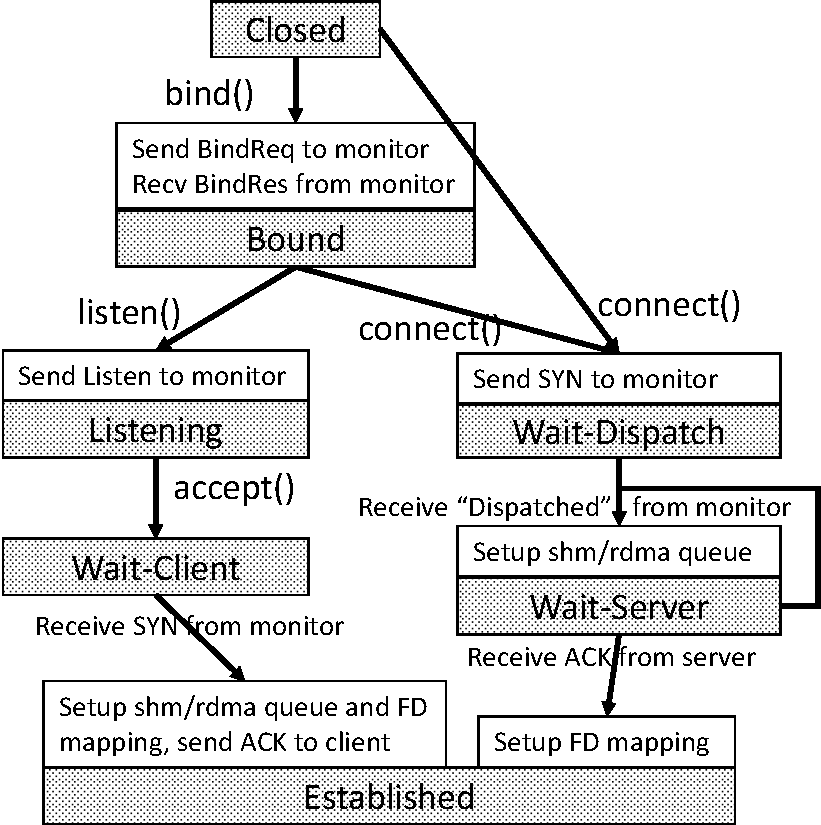
\includegraphics[width=0.6\textwidth]{images/conn-setup-new}
	\caption{\libipc{} 中连接建立过程的状态机。}
	\label{socksdirect:fig:conn-setup}
\end{figure}


\subsubsection{文件描述符重映射表}
\label{socksdirect:subsubsec:fd-remapping-table}



套接字文件描述符和其他文件描述符(例如磁盘文件)共享命名空间,Linux总是分配最低可用文件描述符。
为了保留这种语义而不在内核中分配虚拟文件描述符,\libipc {}拦截所有与文件描述符相关的Linux API并维护\emph {文件描述符重映射表}以将每个应用文件描述符映射到用户空间套接字对象或内核文件描述符。
当文件描述符关闭时,\libipc {}将其放入\emph {文件描述符回收池}。
在文件描述符分配时,\libipc {}首先尝试从池中获取文件描述符。
如果池为空,则通过递增\emph {文件描述符分配计数器}来分配新的文件描述符。
文件描述符回收池和分配计数器在进程中的所有线程之间共享。

\subsubsection{连接建立}


图 \ref {socksdirect:fig:conn-setup}显示了连接建立过程。

\textbf{绑定。}
创建套接字后,应用程序调用\texttt {bind}来分配地址和端口。
由于地址和端口是具有权限保护的全局资源,因此分配由监视器协调。
如图 \ref {socksdirect:fig:conn-setup}所示,\libipc {}将请求发送到监视器。
为了隐藏联系监视器的延迟,如果绑定请求不会失败,\libipc {}会立即返回应用程序,例如,当没有为客户端套接字指定端口时。

\textbf{监听。}
当服务器应用程序准备好接受来自客户端的连接时,它会调用\texttt {listen}并通知监视器。
监视器维护每个地址和端口上的侦听进程列表,以分派新连接。


\textbf{连接。}
客户端应用程序调用\texttt {connect}并发送SYN命令以通过SHM队列进行监视。
现在,监视器需要将新连接分派给侦听应用程序。
在Linux中,新的连接请求在内核的\emph {积压}(backlog)中排队。
每次服务器应用程序调用\texttt {accept}时,它都会访问内核以从积压中出列,这需要同步并增加延迟。
相反,\sys{} 为每个侦听套接字的线程维护一个每个监听器的积压。
监视器以循环方式将SYN分发给侦听器线程。

当侦听器不接受新连接时,调度与侦听器的连接可能会导致饥饿。
\sys{} 使用 \emph {work stealing}方法。
当监听器在积压为空时调用\texttt {accept}时,它会请求监视器窃取其他人的积压。
为了避免侦听器和监视器之间的争用,监视器向侦听器发送请求以从积压中窃取。

\textbf {建立点对点队列。}
客户端和服务器应用程序第一次通信时,服务器监视器可帮助它们建立直接连接。
对于主机内部,监视器分配SHM队列并将SHM密钥发送到客户端和服务器应用程序。
对于主机间,客户端和服务器监视器建立新的RDMA QP,并将本地和远程密钥发送到相应的应用程序。
为了减少延迟,当SYN命令分发到监听器的待办事项时,监视器会建立对等队列。
但是,如果SYN被另一个侦听器窃取,则需要在客户端和新侦听器之间建立新队列,如图 \ref {socksdirect:fig:conn-setup}中的Wait-Server状态所示。

\textbf {连接建立的最后步骤。}
服务器设置对等队列后,如图 \ref {socksdirect:fig:conn-setup}左侧所示,服务器应用程序向客户端发送ACK。 ACK包含SYN请求中的客户端文件描述符及其分配的服务器文件描述符。
与TCP握手类似,服务器应用程序可以在发送ACK后将数据发送到队列。
当客户端收到ACK时,如图 \ref {socksdirect:fig:conn-setup}右侧所示,它设置文件描述符映射并可以开始发送数据。


\subsubsection{与常规 TCP/IP 对端的兼容性}


为了与不支持\sys {}和RDMA的对等端兼容,需要检测\sys {}功能并回退到TCP / IP。
但是,Linux不支持向TCP SYN和ACK数据包添加特殊选项。
由于中间盒和网络重新排序,使用另一个端口(例如LibVMA~ \cite {libvma})也是不可靠的。
为此,首先使用内核原始套接字直接发送带有特殊选项的SYN和ACK数据包,如果不存在特殊选项,则回退到内核TCP / IP套接字。

在客户端,监视器通过网络发送带有特殊选项的TCP SYN数据包。
如果对等体具有\sys {}能力,则其监视器将接收特殊SYN并且知道客户端具有\sys {}能力。
然后,服务器使用特殊选项响应SYN + ACK,包括设置RDMA连接的凭据,以便两个监视器之后可以通过RDMA进行通信。
如果客户端或服务器监视器发现对等方是常规TCP / IP主机,它将使用TCP连接修复 \cite {tcp-connection-repair}在内核中创建已建立的TCP连接。
然后监视器通过Unix域套接字将内核文件描述符发送到应用程序,\libipc {}可以使用内核文件描述符进行未来的套接字操作。


一个棘手的问题是接收的数据包被传递到原始套接字和内核网络堆栈,并且内核将使用RST响应,因为这样的连接不存在。
为避免此行为,监视器会安装\emph {iptables}规则来过滤此类出站RST数据包。

%\begin{figure}[htbp]
%	\centering
%	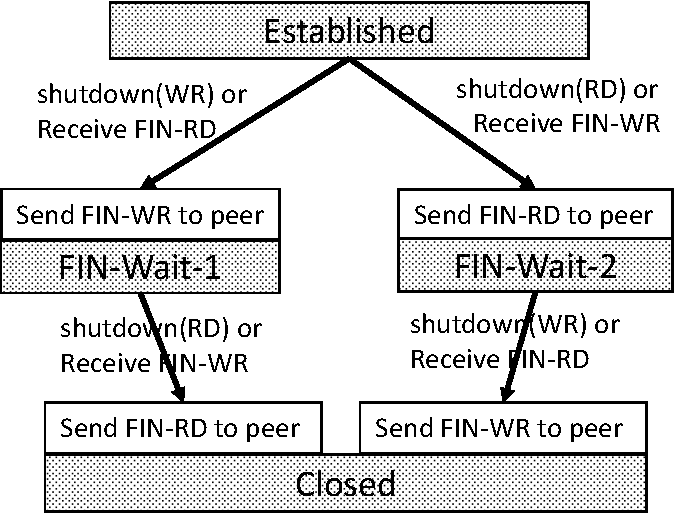
\includegraphics[width=0.25\textwidth]{images/conn-close-new}
%	
%	\caption{State machine of connection close in \libipc{}.}
%	\label{socksdirect:fig:conn-close}
%\end{figure}


\subsubsection{连接关闭}



当应用程序调用\texttt {close}时,\libipc {}会从重映射表中删除文件描述符。
然而,套接字数据可能仍然有用,因为文件描述符可以与其他进程共享,并且缓冲区中可能存在未发送的数据。
\libipc{} 跟踪每个套接字的引用计数,它在fork上递增,在close时递减。
为了推出未发送的数据,需要在对等体之间进行握手,类似于TCP close。
因为套接字是双向的,所以\texttt {close}在发送和接收方向上相当于\texttt {shutdown}。
当应用程序关闭连接的一个方向时,它会向对等方发送\emph {shutdown message}。
对等体以关闭消息响应。
当\libipc {}在两个方向上收到关闭消息时,将删除套接字。


\iffalse

\textbf{\texttt{Bind} and \texttt{listen}.}
A \emph{server} process \texttt{bind}s a socket and needs to detect IP and port conflict. In this case, \texttt{bind} is non-partitionable and goes to the monitor. The monitor also listens on the IP and port in a user-space TCP/IP stack (\textit{e.g.} mTCP~\cite{jeong2014mtcp}, LibVMA~\cite{libvma} or Seastar~\cite{seastar}) to receive connections from other hosts.

A \emph{client} process typically \texttt{bind}s without specifying IP and port, so we need to allocate a unique IP and port for it. For scalability, we partition the loopback IP address space (127.0.0.0/8) and each process allocates IP and port in its range.

\textbf{\texttt{Connect} and \texttt{accept}.}
When a client process connects to a server process on the same host, it sends a \textit{connect request} to the monitor via shared memory queue. When the server process is on another host, it creates a \textit{bootstrap TCP socket} with a special option via the user-space TCP/IP stack. If the server host supports the option, it is a \sys host and its monitor establishes an RDMA connection to the client to speedup later communications. Otherwise, the client process keeps using the bootstrap TCP socket for compatibility.

On a server host, the monitor distributes connect requests to server processes in a round-robin order, and a \textit{backlog} is maintained in each process. If the client is TCP only, the monitor proxies messages between the server process and the user-space TCP/IP stack. If the client is intra-server or RDMA capable, and it is the first time for the client and server processes to communicate, the monitor creates an inter-process queue for the process pair and sends the credentials to both processes via bootstrap sockets. After a server process \texttt{accept}s a connection in the backlog, it sends a message to the client via inter-process queue to create an 文件描述符 mapping, then the socket is ready for data transmission. As Figure~\ref{socksdirect:fig:conn-setup} shows, connection creation takes three inter-process delays.

Distributing connection to listeners may lead to starvation when a listener does not \texttt{accept} new connections. We devise a \textit{work stealing} approach. When a listener \texttt{accept}s from empty backlog, it requests the monitor to steal from others' backlog. To avoid polling empty backlogs, each listener notifies the monitor when its backlog becomes empty. To avoid contention between a listener and monitor, the monitor sends a request to the listener rather than stealing from the backlog directly.

%\subsubsection{Connection Close}

\textbf{\texttt{Close} and \texttt{shutdown}.}
Connection close is a peer-to-peer operation because only the peer process needs to be notified. If 文件描述符 is deleted immediately after \texttt{close}, a new connection may reuse the 文件描述符 while the peer process might not yet have received the close event thus sends data to the wrong connection. To avoid this, we require a handshake between peers.
Because socket is bidirectional, \texttt{close} is equivalent to \texttt{shutdown} on both send and receive directions.
When application shuts down one direction of a connection, it sends a \textit{shutdown message} to the peer. The peer responds with a shutdown message. A process deletes an 文件描述符 when it receives shutdown messages in both directions.

%In order to achieve high scalability, we separate scalable operations to different processes. To avoid the overhead of contention, \libipc enable the file descriptor allocation by individual process and when a connection is setup, the other peer of the connection gets notified of the file descriptor number by message passing. Since we treat different threads in one process as different processes, we allocate file descriptor of different ranges to each of them to avoid collision. Since file descriptor is managed separately by each process, it is possible that a file descriptor is reused after the connection is closed. Our solution is that resources of a file descriptor is not released until an ACK is received for the close operation.

%Generally, each process in our design is treated as an endpoint in the network. Figure \ref{socksdirect:fig:conn-setup-close} shows the process of connection setup and close. When \textit{socket} is called, the process itself allocate per fd resources. When \textit{listen} is called, monitor is notified of port occupation. During the \textit{connect} operation, monitor first chooses one of the processes listen on this port then coordinates the creation of the shared memory between the two processes and notifies each other of the new connection. When \textit{close} happens, both of the endpoint notify each other and monitor is responsible to destroy the shared memory between them. 

\fi

\section{评估}
\label{socksdirect:sec:evaluation}

\begin{figure*}[htbp]
		\centering
		\subfloat[单机内吞吐量。]{                    
			%\begin{minipage}{0.4\textwidth}
			\centering
			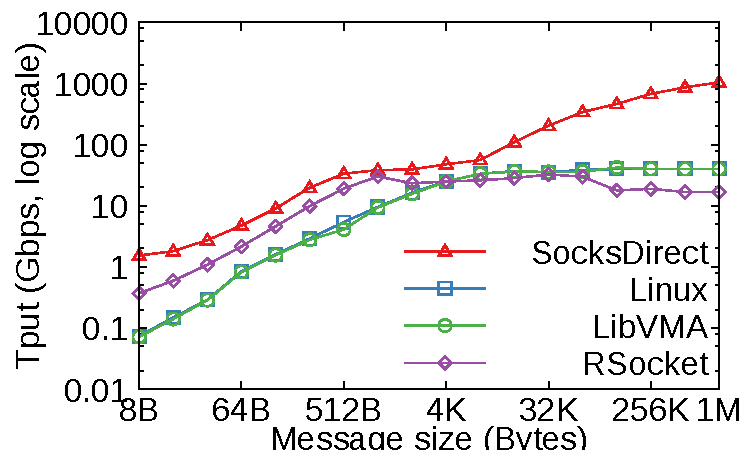
\includegraphics[width=0.5\textwidth]{eval/microbenchmark/msgsize-ipc-tput.pdf}
			\label{socksdirect:fig:eval-msgsize-ipc-tput}
			%\end{minipage}
		}
		\subfloat[单机内延迟。]{
			%\begin{minipage}{0.4\textwidth}
			\centering 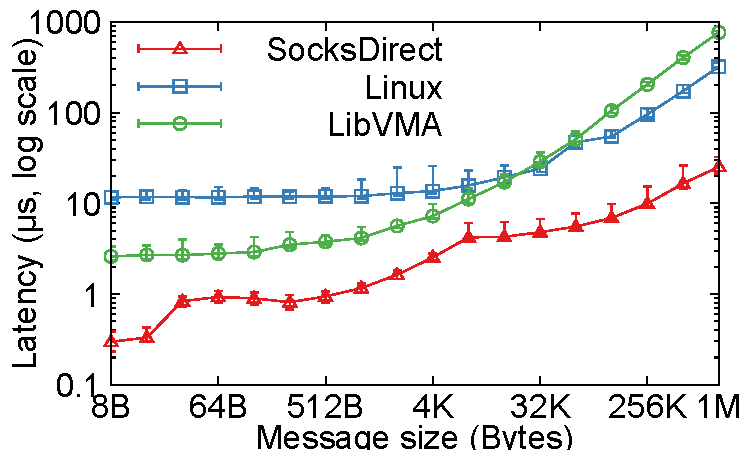
\includegraphics[width=0.5\textwidth]{eval/microbenchmark/msgsize-ipc-lat.pdf}
			\label{socksdirect:fig:eval-msgsize-ipc-lat}
			%\end{minipage}
		}
		
		\caption{不同消息大小下的单机内通信单核消息性能。}
		\label{socksdirect:fig:eval-msgsize-intra}
\end{figure*}


\begin{figure*}[htbp]
		\centering
		\subfloat[跨主机吞吐量。]{
			%\begin{minipage}{0.4\textwidth}
			\centering 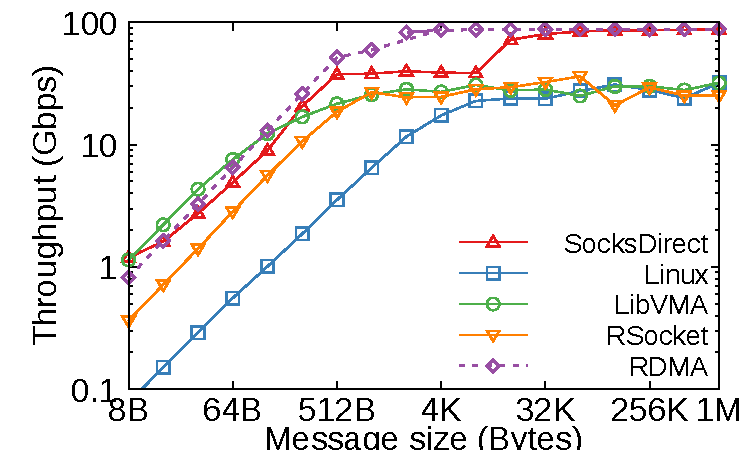
\includegraphics[width=0.5\textwidth]{eval/microbenchmark/msgsize-network-tput.pdf}
			\label{socksdirect:fig:eval-msgsize-network-tput}
			%\end{minipage}
		}
		\subfloat[跨主机延迟。]{
			%\begin{minipage}{0.4\textwidth}
			\centering 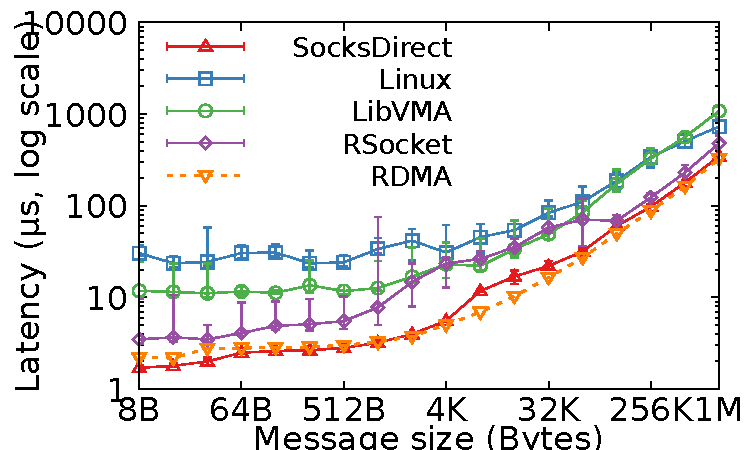
\includegraphics[width=0.5\textwidth]{eval/microbenchmark/msgsize-network-lat.pdf}
			\label{socksdirect:fig:eval-msgsize-network-lat}
			%\end{minipage}
		}
		
		\caption{不同消息大小下的跨主机通信单核消息性能。}
		\label{socksdirect:fig:eval-msgsize-inter}
\end{figure*}

\begin{figure*}[htbp]
		\subfloat[单机内吞吐量。]{                    
			%\begin{minipage}{0.4\textwidth}
			\centering
			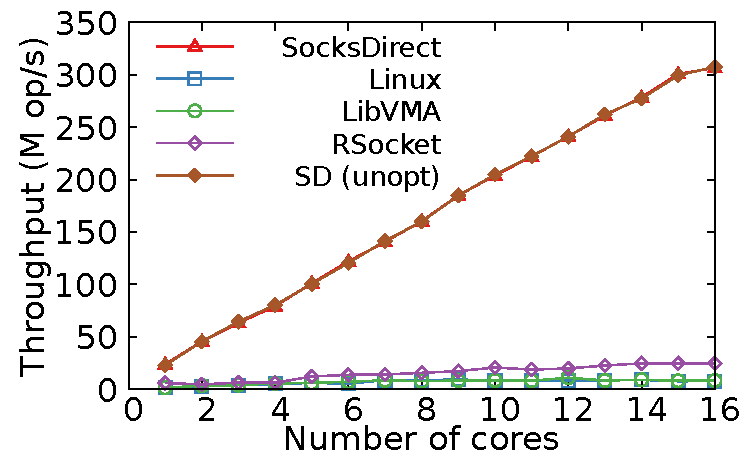
\includegraphics[width=0.5\textwidth]{eval/microbenchmark/corenum-IPC-tput.pdf}
			\label{socksdirect:fig:eval-cornum-ipc}
			%\end{minipage}
		}
		\subfloat[跨主机吞吐量。]{
			%\begin{minipage}{0.4\textwidth}
			\centering 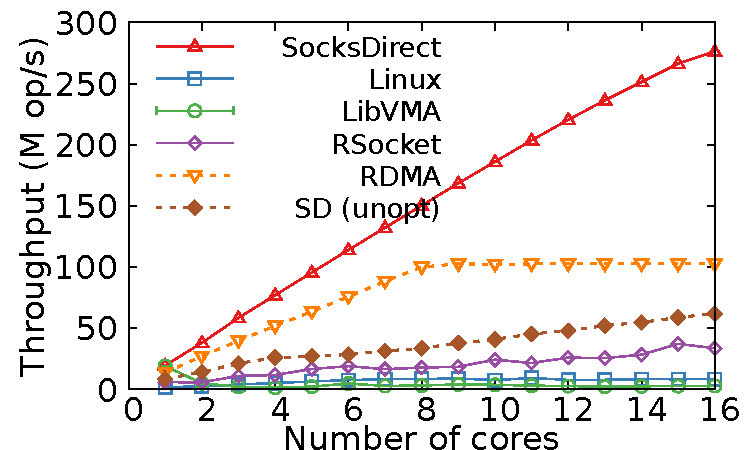
\includegraphics[width=0.5\textwidth]{eval/microbenchmark/corenum-network-tput.pdf}
			\label{socksdirect:fig:eval-cornum-network}
			%\end{minipage}
		}
		
		\caption{不同 CPU 核数下的 8 字节消息吞吐量。}
		\label{socksdirect:fig:eval-corenum-tput}
\end{figure*}

\begin{figure*}[htbp]
		\centering
		\subfloat[单机内吞吐量。]{                    
			%\begin{minipage}{0.4\textwidth}
			\centering
			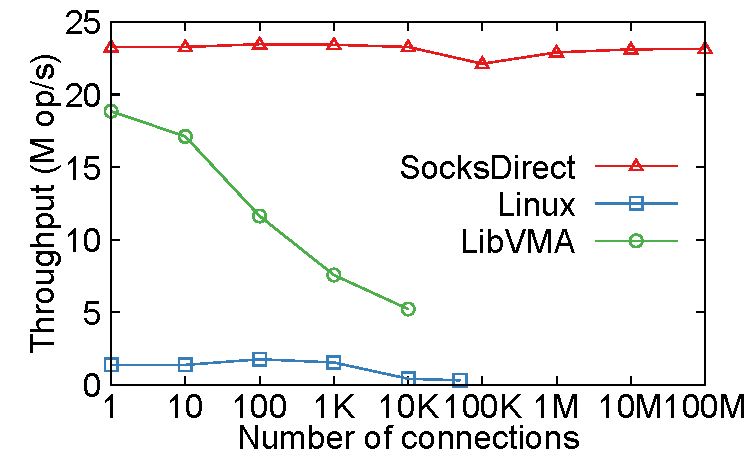
\includegraphics[width=0.5\textwidth]{eval/microbenchmark/connnum-ipc-tput.pdf}
			\label{socksdirect:fig:eval-connnum-ipc-tput}
			%\end{minipage}
		}
		\subfloat[跨主机吞吐量。]{
			%\begin{minipage}{0.4\textwidth}
			\centering 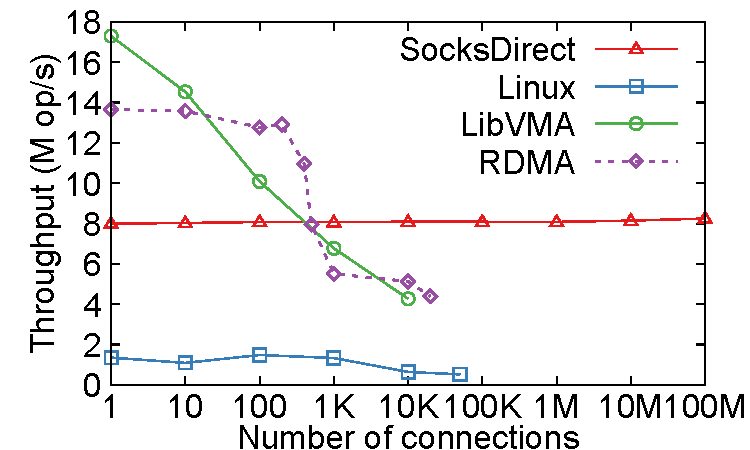
\includegraphics[width=0.5\textwidth]{eval/microbenchmark/connnum-network-tput.pdf}
			\label{socksdirect:fig:eval-connnum-network-tput}
			%\end{minipage}
		}
		
		\caption{不同并发连接数量下的单核吞吐量。}
		\label{socksdirect:fig:eval-connnum-tput}
\end{figure*}

%\begin{figure}[htpb]
%	\centering
%	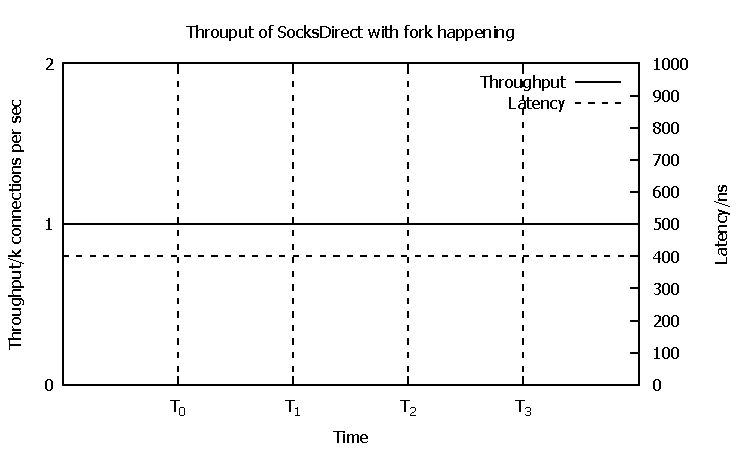
\includegraphics[width=\columnwidth]{eval/microbenchmark/fork-tput.pdf}
%	\caption{Throughput of SocksDirect with fork happening}
%	\label{socksdirect:fig:eval-fork-tput}
%\end{figure}

我们在三个组件中实现\sys :一个用户空间库\libipc {}和一个带有17K行C ++代码的监控守护进程,以及一个支持零拷贝的修改过的RDMA NIC驱动程序。 我们在以下方面评估\sys :

\parab {有效地为主机内套接字使用共享内存。}
对于8字节消息,\sys 实现0.3 $\mu$s RTT和每秒23~M消息的吞吐量。 对于大型消息,\sys 使用零拷贝来实现Linux的1/13延迟和26x吞吐量。

\parab {有效地使用RDMA进行主机间套接字。}
\sys 达到1.7 $\mu$s RTT,接近原始RDMA性能。
零拷贝时,一个连接会使100~Gbps链路饱和。

%\parab{Robust with number of connections.}
%The performance above can be maintained with up to 100 million connections.

%\parab{Corner-case operations does not affect long-term performance.}
%After corner-case operations such as \texttt{fork}, the performance recovers quickly.

\parab {可扩展核心数。}
随着核心数量的增加,吞吐量几乎可以线性扩展。


\parab {使用未经修改的端到端应用程序显着加速。}
例如,\sys  {}将Nginx HTTP请求延迟减少5.5倍到20倍。


\subsection{方法}
\label{socksdirect:subsec:methodology}

我们使用两个Xeon E5-2698 v3 CPU,256~GiB内存和一个Mellanox ConnectX-4网卡评估服务器上的\sys 。服务器与Arista 7060CX-32S 100G交换机互连 \cite {arista-7060cx}。我们使用Ubuntu 16.04和Linux 4.15,RoCEv2用于RDMA,每64条消息轮询完成队列。
每个线程都固定在CPU内核上。在收集数据之前,我们会进行足够的预热测试。
对于延迟,我们构建一个乒乓应用程序并报告平均往返时间,误差条代表1%和99%百分位数。
对于吞吐量,一方保持发送数据而另一方不断接收数据。
我们将比较Linux,原始RDMA写动词,Rsocket~ \cite {rsockets}和LibVMA~ \cite {libvma},这是针对Mellanox NIC优化的用户空间TCP / IP堆栈。
我们没有评估mTCP~ \cite {jeong2014mtcp},因为底层DPDK库对我们的NIC的支持有限。由于批处理,mTCP具有比RDMA高得多的延迟,报告的吞吐量为每秒1.7~M包~~ \cite {kalia2018datacenter}。

\subsection{微基准测试}
\label{socksdirect:subsec:microbenchmark}

\subsubsection{延迟和吞吐量}



图 \ref {socksdirect:fig:eval-msgsize-intra}显示了一对发送方和接收方线程之间的主机内套接字性能。
对于8字节消息,\sys 实现0.3 $ \mu $ s往返延迟(Linux的1/35)和每秒23~M消息吞吐量(Linux的20倍)。
相比之下,一个简单的SHM队列具有0.25 $ \mu $ s往返延迟和27~M吞吐量,表明\sys 增加了很少的开销。
RSocket具有6x延迟和1/4吞吐量的\sys  {},因为它使用NIC转发主机内数据包,这会导致PCIe延迟。
LibVMA只是将内核TCP套接字用于主机内部。
\sys  {}的单向延迟为0.15 $ \mu $ s,甚至低于内核交叉(0.2 $ \mu $ s)。基于内核的套接字需要在发送方和接收方都进行内核交叉。

由于内存复制,对于8~KiB消息,\sys 的吞吐量仅比Linux高60%,延迟低4倍。对于大小至少为16~KiB的消息,\sys 使用页面重映射来实现零拷贝。
对于1~miB消息,\sys 比Linux具有1/13延迟和26x吞吐量。
由于事件通知延迟,RSocket的延迟不稳定,在某些情况下甚至可能比Linux大。


图 \ref {socksdirect:fig:eval-msgsize-inter}显示了一对线程之间的主机间套接字性能。
对于8字节消息,\sys 实现每秒18M消息吞吐量(Linux的15倍)和1.7美元/秒的延迟(Linux的1/17)。
吞吐量和延迟接近原始RDMA写操作(如虚线所示),它没有套接字语义。
由于批处理,\sys  {}对于8字节消息的吞吐量甚至高于RDMA。
对于16到128字节的消息,LibVMA还使用批处理来实现比\sys  {}更好的吞吐量,但延迟是\sys  {}的7倍。
对于小于8~KiB的消息大小,主机间RDMA的吞吐量略低于主机内SHM,因为环形缓冲区结构是共享的。
对于512B到8KiB消息,\sys  {}受数据包复制的限制,但由于缓冲管理开销减少,仍然比RSocket和LibVMA更快。
对于零拷贝消息($\ge$ 16 KiB),\sys  {}使网络带宽饱和,其具有所有比较工作的3.5倍吞吐量和RSocket的72%延迟。



\begin{figure}[htbp]
		%\centering
		%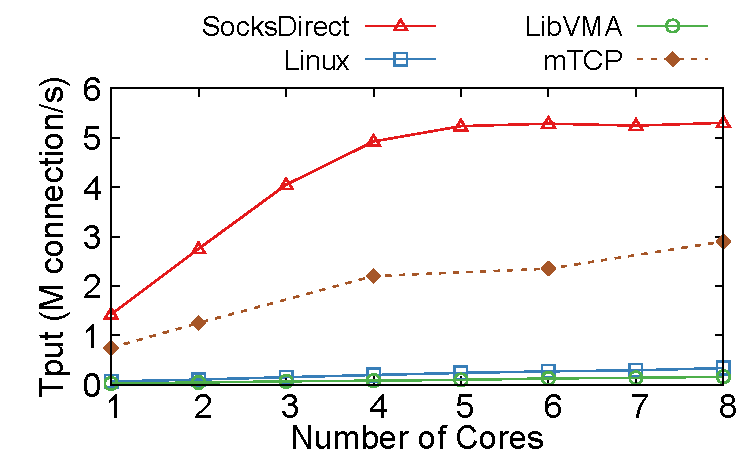
\includegraphics[width=\textwidth]{eval/microbenchmark/conn-setup-tput.pdf}
		%
		%\caption{Connection creation throughput with number of cores.}
		%\label{socksdirect:fig:eval-conn-setup-tput}
		
		%\begin{minipage}{0.4\textwidth}
		\centering 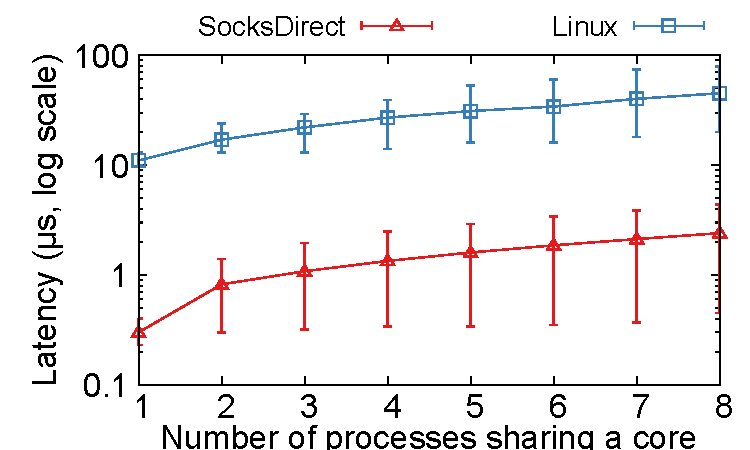
\includegraphics[width=0.5\textwidth]{eval/microbenchmark/sharecore-lat.pdf}
		
		\caption{多进程共享 CPU 核的消息处理延迟。}
		\label{socksdirect:fig:eval-context-switch}
		%\end{minipage}
\end{figure}
\begin{figure}[htbp]
				\centering 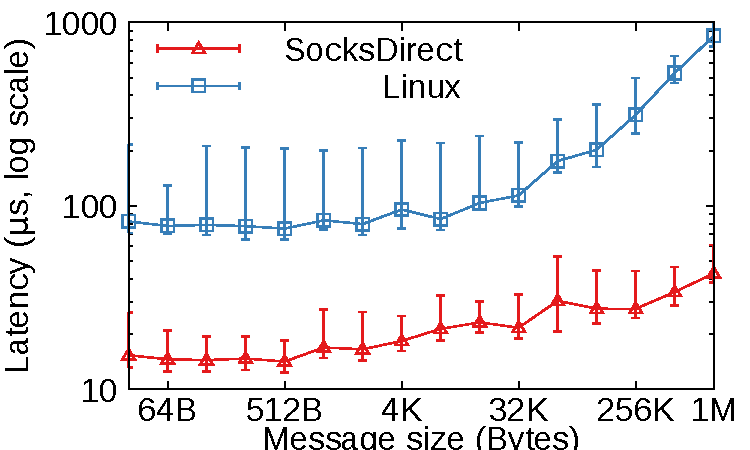
\includegraphics[width=0.5\textwidth]{eval/web/msgsize-clocal-lat.pdf}
		
		\caption{Nginx HTTP 请求端到端延迟。}
		\label{socksdirect:fig:eval-nginx}
\end{figure}
\begin{figure}[htbp]
		\centering
		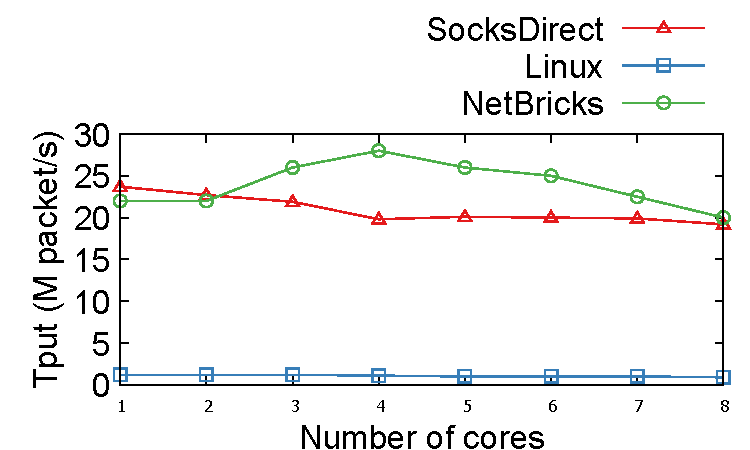
\includegraphics[width=0.5\textwidth]{eval/microbenchmark/nfv-tun-tput.pdf}
		
		\caption{网络功能流水线的吞吐量。}
		\label{socksdirect:fig:eval-tun-tput}
		%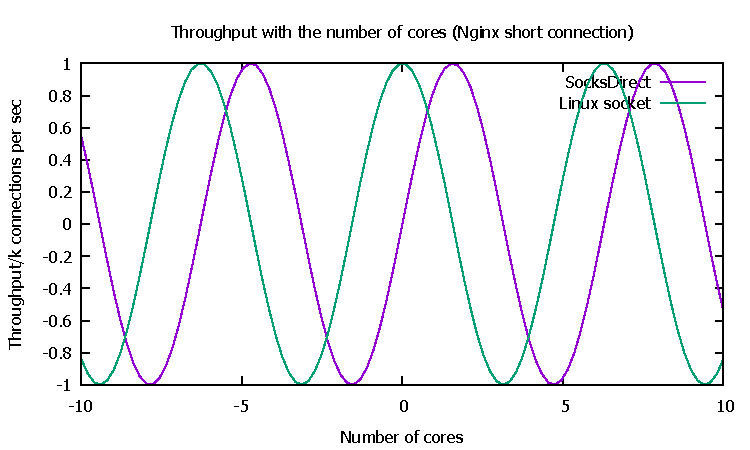
\includegraphics[width=\textwidth]{eval/microbenchmark/nginx-short-tput.pdf}
		%
		%\label{socksdirect:fig:eval-nginx-short}
		%\caption{Nginx throughput.}
		
		%\centering 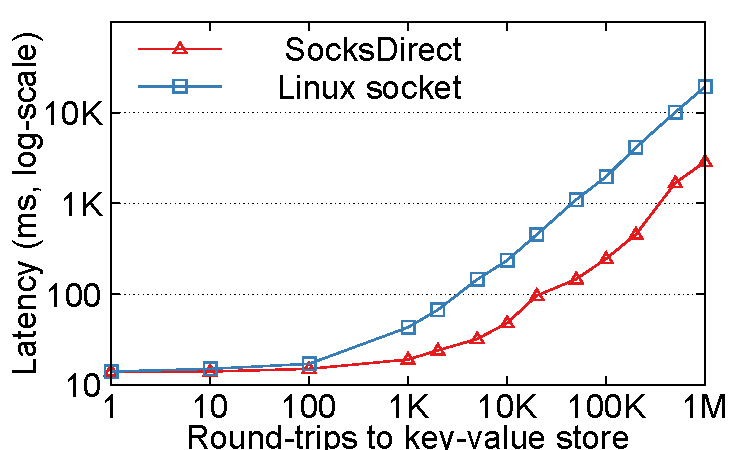
\includegraphics[width=\textwidth]{eval/microbenchmark/nginx-multiround-tput.pdf}
		%
		%\caption{End-to-end HTTP request latency of a web service.}
		%\label{socksdirect:fig:eval-nginx-multiround}
		
		%\centering
		%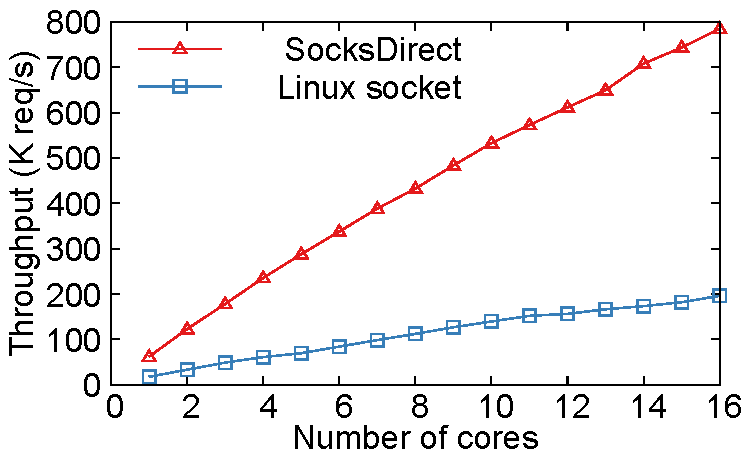
\includegraphics[width=\textwidth]{eval/microbenchmark/corenum-http-tput.pdf}
		%
		%\caption{Multi-core scalability of HTTP backend service throughput.}
		%\label{socksdirect:fig:eval-http-tput}
\end{figure}


\subsubsection{多核可扩放性}

%Figure~\ref{socksdirect:fig:eval-connnum-tput} shows the throughput with different number of concurrent connections.
%We establish connections between two processes before testing, then send and receive data from the connections in a round-robin order.
%\sys  can support more than 100 million concurrent connections with 16~GiB of memory, and the throughput does not degrade under such high concurrency.
%\sys  achieves connection stability by multiplexing connections via a single queue.
%In comparison, the performance of RDMA, LibVMA and Linux drops quickly as the number of connections increase. There is a sharp performance drop with more than 512 RDMA connections, because the RDMA transport states saturate the NIC cache. Although LibVMA and Linux do not use RDMA as transport, they maintain per-FD buffers, which lead to CPU cache and TLB miss with thousands of connections. Furthermore, LibVMA installs flow steering rules to NIC for each connection, which also leads to NIC cache miss.




\sys 实现了主机内和主机间套接字的几乎线性可扩展性。
对于主机内套接字,\sys 在16对发送器和接收器核心之间提供每秒306~M消息的吞吐量,这是Linux的40倍和RSocket的30倍。
LibVMA回退到Linux用于主机内套接字。
使用RDMA作为主机间套接字,\sys 使用批处理以16个内核实现每秒276~M个消息的吞吐量,这是我们RDMA网卡的消息吞吐量的2.5倍。
由于缓冲区管理的可扩展性有限,RSocket的主机内部为24~M,主机间为33~M。
由于共享NIC队列上的锁争用,与单线程相比,LibVMA的吞吐量减少到两个线程的1/4,而三个和更多线程的1/10。
Linux吞吐量从1到7个核心线性扩展,并在环回或具有更多核心的NIC队列上出现瓶颈。

%The multi-thread scalability of \sys  attributes to the partitioning of states and removal of synchronization.
%We can also see that shared memory communication has 5x throughput than RDMA.% Using RDMA NIC for intra-host socket would meet this bottleneck and thus not scalable.

%Figure~\ref{socksdirect:fig:eval-conn-setup-tput} shows the throughput of connection creation with different number of cores. Each core can create 1.4~M new connections per second, which is 20x of Linux and 2x of mTCP~\cite{jeong2014mtcp}. The upper bound is 5.3~M connections per second, where the monitor becomes a bottleneck.

最后,我们评估共享核心的多个线程的性能。 每个线程都需要等待轮到它来处理消息。
如图 \ref {socksdirect:fig:eval-context-switch}所示,尽管消息处理延迟几乎与活动进程的数量呈线性增长,但它仍然是Linux的1/20到1/30。



%Finally, we benchmark the throughput and latency after \texttt{fork} and other corner-case operations. Initially, there is only one pair of sender and receiver. At time $T_0$, receiver forks, and the parent process keeps receiving. At time $T_1$, the child process begins to receives takes over the socket. At time $T_2$, sender forks, and only the parent sends. At time $T_3$, the child sender also starts sending. We find that both throughput and latency resume to initial maximal performance within 1~ms after each event.

%!TEX root=main.tex
\section{应用}
\label{clicknp:sec:application}

为了评估 \name 的灵活性,我们基于 \name 开发了五个常见的网络功能,可以在我们的测试床中运行。
表 \ref {clicknp:tab:applications} 总结了每个网络功能中包含的元件数量和总代码行数,包括所有元件规范和配置文件。
经验证实,\name 的模块化架构极大地改善了代码重用并简化了新网络功能的构建。
如表 \ref {clicknp:tab:elements} 所示,在许多应用程序中有很多机会重用一个元件,例如,本文(A1-5)中所有五个网络功能都使用了L4\_Parser。
每个网络功能可能需要1个左右的时间才能让一个程序员进行开发和调试。
联合CPU / FPGA处理的能力也将极大地帮助调试,因为可以将有问题的元件移动到CPU,以便轻松地打印日志来跟踪问题。

下文将详细讨论这些网络功能。

\textbf {A1. 数据包生成器(PktGen)和捕获(PktCap)。}
PktGen可以根据不同的配置文件生成各种流量模式。
它可以生成不同大小的流,并根据给定的分布安排它们在不同的时间开始。
生成的流可以进一步通过不同的流量整形器来控制流速及其突发性。
PktCap只是将收到的所有数据包重定向到 \textit {logger} 元件,这些元件通常位于主机中。
由于单个记录器无法充分利用PCIe I / O通道容量,因此PktCap在FPGA中具有接收端缩放(RSS)元件,以根据流5元组的散列将数据包分发到多个记录器。
由于PCIe通道的容量小于40G 网卡的容量,添加了一个\textit {提取器}(extractor)元件,它只提取数据包的重要字段(例如,如果有5个元组,DSCP和VLAN标记),并转发这些字段(总共16B) ,以及跨PCIe的记录器元件的时间戳(4B)。
PktCap就是一个展示联合CPU / FPGA处理重要性的例子。
与FPGA相比,CPU具有更多的内存用于缓冲,并且可以轻松访问其他存储,例如,文献 \cite{lee2015flosis} 中的HDD / SSD驱动器,因此在CPU上运行记录器更有意义。


\textbf {A2. OpenFlow 防火墙(OFW)。}
Openflow~\cite {mckeown2008openflow} 防火墙支持流的精确匹配和通配符匹配。
精确匹配表是使用Cuckoo Hashing \cite{cuckoo} 实现的,包含与流5元组匹配的128K条目。
模糊匹配匹配基于TCAM。
但是,具有512个104位条目的简单TCAM实现占用了FPGA的65%逻辑资源。
相反,本章使用基于BRAM的TCAM \cite {jiang2013scalable}。
基于BRAM的TCAM将搜索密钥分解为8位密钥,并使用它们来寻址查找表,这些表将内存换成逻辑区域。具有2K条目的BRAM TCAM需要14%逻辑和43%的BRAM。
此外,本文设计了 HashTCAM,以利用流表中的许多条目共享相同的位掩码这一事实。
HashTCAM将表空间划分为许多较小的哈希表,每个哈希表都与一个位掩码相关联。
在查找哈希表之前,任何传入的数据包都将首先执行“和”操作。
表中的每个条目也与优先级相关联。
仲裁器(multiplexer)选择具有最高优先级的匹配条目。
HashTCAM在功能和区域成本之间有更好的权衡。
具有16K流条目和16个不同位掩码的HashTCAM(类似于Broadcom Trident II~\cite {broadcomethernet})需要19%逻辑和22%BRAM。
管理器程序总是尝试根据其位掩码对规则进行分组,并将具有大多数规则的组放入HashTCAM。
然后将其余规则放入基于BRAM的TCAM中,这些规则不适合HashTCAM中的任何组。


\textbf{A3. IPSec网关(IPSecGW)。}
软件网络功能的一个问题是,当数据包需要一些计算密集型处理时,CPU很快就会成为瓶颈,例如,IPSec \cite {packetshader}。
IPSec数据面需要使用AES-256-CTR加密和SHA-1身份验证处理IPSec数据包。
如 \S \ref {clicknp:subsec:lib} 所示,单个AES\_CTR元件只能实现27.8~Gbps的吞吐量。因此,需要两个AES\_CTR元件并行运行以实现线速率。
然而,SHA-1很棘手。 SHA-1将数据包分成较小的数据块(64B)。
虽然一个数据块中的计算可以流水线化,但是一个IP数据包内的连续块之间存在依赖关系 - 下一个块的计算无法在前一个块完成之前开始!
如果按顺序处理这些数据块,吞吐量将低至1.07 Gbps。
幸运的是,可以利用不同数据包之间的并行性。
虽然当前数据包的数据块的处理仍在进行,但提供了不同数据包的数据块。
由于这两个数据块没有依赖关系,因此可以并行处理它们。
为了实现这一点,我们设计了一个名为 \textit {reservo} 的新元件(保留站的简称),它可以缓冲多达64个数据包,并为SHA-1元件调度独立的块。在计算了一个数据包的签名之后,\textit {reservo} 元件将它发送到将SHA-1 HMAC附加到数据包的下一个元件。
还有一件棘手的事情。
虽然SHA-1元件具有固定的延迟,但数据包的总延迟是不同的,即与数据包大小成比例。
当在SHA-1计算中调度多个分组时,这些分组可能是无序的,例如,大分组后面的较小分组可能更早地完成。
为了防止这种情况,在SHA-1元件之后进一步添加了一个\textit {reorder buffer}元件,该元件存储无序数据包并根据数据包的序列号恢复原始顺序。

\textbf {A4. L4负载平衡器(L4LB)。}
L4 负载平衡器根据Ananta~ \cite {ananta}中的\textit {multiplexer}(MUX)实现。
MUX服务器基本上查看数据包标头,并查看是否已为该流分配了\textit {直接地址}(DIP)。
如果是,则通过NVGRE隧道将分组转发到由DIP指示的服务器。否则,MUX服务器将调用本地控制器为流分配DIP。
MUX服务器中需要按流状态。
由于存在故障并且避免黑洞需要即时更改后端服务器列表,因此无法使用基于散列的ECMP。此外,高级LB还可能需要负载感知平衡。
流表用于记录流向其DIP的映射。
为了处理数据中心的大流量,它需要L4LB在流表中支持多达3200万个流。
显然,如此大的流量表不能适应FPGA的BRAM,必须存储在板载DDR存储器中。
但是,访问DDR内存很慢。
为了提高性能,在BRAM中创建了一个带有16K高速缓存行的4路关联流缓存。最近最少使用(LRU)算法用于替换流缓存中的条目。

在本章的实现中,传入的数据包首先传递一个\textit {解析器}(parser)元件,该元件提取5元组并将它们发送到\textit {流缓存}(flow cache)元件。
如果在流缓存中找不到流,则将数据包的元数据转发到全局流表,该表读取DDR中的完整表。
如果仍然没有匹配的条目,则该数据包是流的第一个数据包,并且请求被发送到\textit {DIPAlloc}元件,以根据负载平衡策略为该流分配DIP。
确定DIP后,将一个条目插入到流表中。

在确定分组的DIP之后,封装元件将检索下一跳信息,例如IP地址和VNET ID,并相应地生成NVGRE封装的分组。
对于流的剩余分组,从流状态提取DIP。
如果收到FIN数据包或发生超时,则流条目将无效
在从流中接收任何新数据包之前。
在确定DIP之后,从BRAM检索下一跳元数据并封装NVGRE头以将分组引导到分配的DIP。

除了\textit {DIPAlloc}元件之外,所有元件都放在FPGA中。
由于只有流的第一个数据包可能会出现\textit {DIPAlloc}并且分配策略也可能很复杂,因此更适合运行
CPU上的\textit {DIPAlloc},是联合CPU-FPGA处理的另一个例子。

%
\egg{
To handle the large traffic volume in datacenters, it requires the L4LB to support up to 32 million flows in the flow table.
Clearly, such a large flow table cannot fit into the BRAM of FPGA, and has to be stored in onboard DDR memory.
Accessing DDR memory is slow. To improve performance, we further create a 4-way associative flow cache in BRAM with 16K 
cache lines. The flow cache is replaced based on the Least Recently Used (LRU) algorithm.
DDR memory access is a fat pipeline stage as shown in Figure \ref{clicknp:fig:unbalance}. We move the DDR access part to a separate element to make the fast path run asynchronously with slow path.}



\textbf {A5. pFabric 流调度程序。}
最后,使用\name 来实现一个最近提出的数据包调度规则--pFabric \cite {pfabric}。
pFabric调度很简单。它只保留浅缓冲区(32个数据包),并始终使具有最高优先级的数据包出列。当缓冲区已满时,优先级最低的数据包将被丢弃。
pFabric显示在数据中心中实现接近最佳的流完成时间。
在原始论文中,作者提出使用二进制比较树(Binary Comparison Tree,BCT)来选择具有最高优先级的数据包。
但是,虽然BCT只需要$O(log_2 N)$个周期来计算最高优先级的数据包,但在连续的选择过程之间存在依赖关系。这是因为只有当前一个选择完成后才能知道最高优先级的数据包,然后才能可靠地启动下一个选择过程。
这种限制要求时钟频率至少为300MHz才能实现40Gbps的线速,这对当前的FPGA平台来说是不可能的。
本文使用不同的方式来实现pFabric调度程序,它更容易并行化。
该方案基于\textit{移位寄存器优先级队列}(shift register priority queue) \cite {moon2000scalable}。
条目以非增加优先级顺序保存在$K$个寄存器中。
出列时,所有条目都向右移动并弹出头部。这只需要1个周期。
对于入队操作,新数据包的元数据将转发到所有条目。
现在,对于每个条目,可以在条目中的分组,新分组和相邻条目中的分组之间执行本地比较。
由于所有局部比较都可以并行进行,因此入队操作也可以在1个周期内完成。
入队和出队操作可以进一步并行化。
因此,可以在一个周期中处理分组。

\iffalse
\textbf{A6. 容错的 LTE SPGW。}

\textbf{A7. 端口扫描检测。}

\textbf{A8. HTTPS RSA 加速。}

\textbf{A9. 正则表达式匹配。}

\textbf{A10. 神经网络推理。}
\fi

\egg{
pFabric \cite{alizadeh2013pfabric} is a near-optimal datacenter transport based on priority scheduling and dropping. Packets are scheduled based on its flow size or remaining flow size in a small queue. Our pFabric scheduler implementation (Figure \ref{clicknp:fig:PFabric}) support 4-giga strict priorities, including a PriorityQueue which deques the packet with highest priority and drops overflow packets with lowest priority, a ReorderQueue to find the earliest packet from the flow with highest priority to avoid starvation and keep packet ordering, and a PacketBuffer to receive packets into buffer and schedule or drop packets out of buffer. Since queue size in a perfectly load balanced fabric should be small, we choose shift register priority queue for maximum throughput and clock frequency.

ReorderQueue is another shift register queue ordered by flow hash. On enque command from PacketBuffer, packet metadata with flow hash $f_{new}$ is enqued to entry $i$ where $f_{i-1} < f_{new} \leq f_{i}$. On deque command from PriorityQueue, the entry $i$ with $f_{i} = f_{deque} < f_{i+1}$ is dequed. Packets with a same flow hash are dequed in the same order as they are enqued.


\begin{figure}[h!]
	\centering
	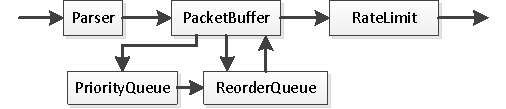
\includegraphics[width=1.0\columnwidth]{image/PFabric}
	\vspace{-0.30in}
	\caption{PFabric Element Graph}
	\vspace{-0.10in}
	\label{clicknp:fig:PFabric}
	%    
\end{figure}
}

\section{连接数可扩放的 RDMA 网卡实现}
\label{socksdirect:sec:discussion}


\begin{figure}[htbp]
	\centering
	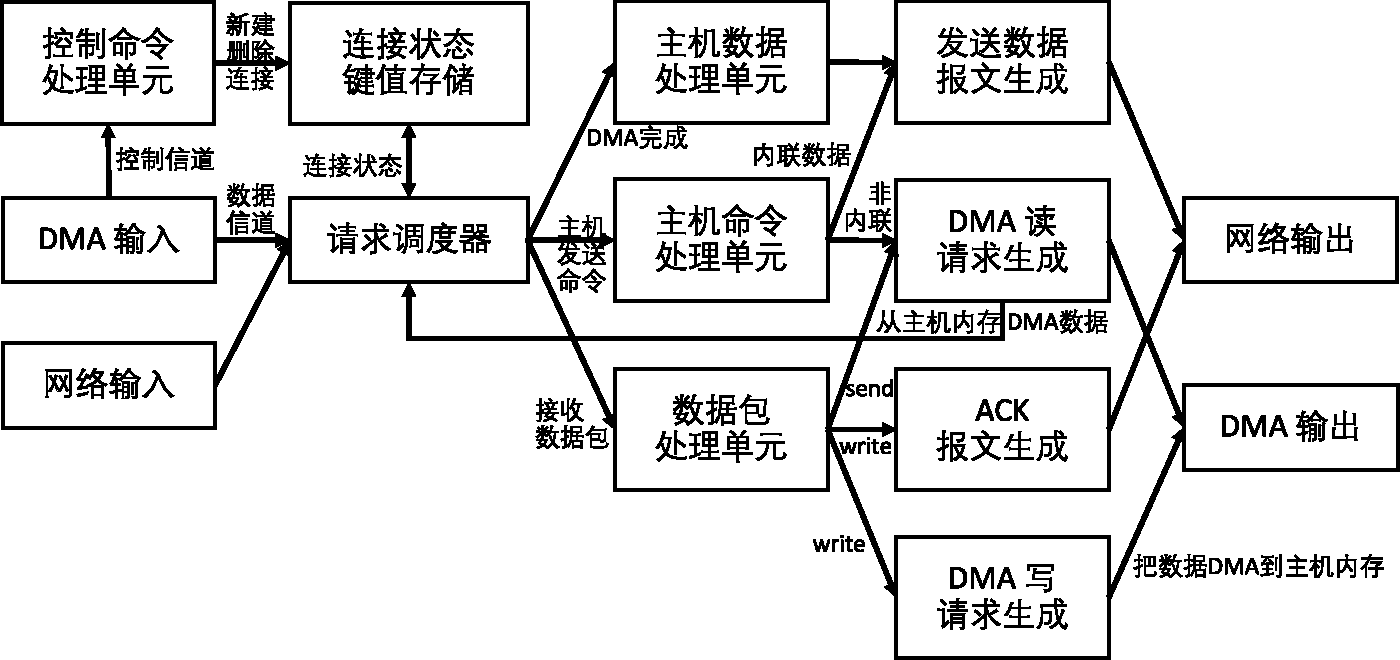
\includegraphics[width=0.9\textwidth]{images/scalable_rdma.pdf}	
	\caption{基于可编程网卡的连接数可扩放 RDMA。}
	\label{socksdirect:fig:scalable-rdma}
\end{figure}

%\textbf{Communicating with TCP/IP peers.}
%We use a user-space networking stack to communicate with regular TCP/IP peers, but the compatibility may be limited~\cite{yasukata2016stackmap}.
%To solve this problem, after receiving the TCP SYN+ACK, the monitor can create an established kernel TCP connection using TCP connection repair~\cite{tcp-connection-repair}.
%Moreover, if the application and monitor share a network namespace, the monitor can send the kernel FD to the application via Unix domain socket, then \libipc{} can use the FD without delegation to the monitor.

%\textbf{Connecting to many RDMA capable hosts.}
%With a lot of hosts, the 网卡 still suffer from performance degradation due to large number of connections.
%In contrast, user-space networking stack alleviates this problem because the 网卡 is stateless.
%We provide a socket option to enable applications to delegate operations to the monitor and use user-space networking stack even if the peer supports RDMA.
%An application can choose to use RDMA for latency sensitive and throughput demanding connections, and user-space networking stack for others.

\parab {扩放到大量连接。}
\sys {}对许多连接的可伸缩性受SHM和RDMA的限制。
为了表明\libipc {}和监视器不是瓶颈,我们运行一个综合实验,在两个重用RDMA QP和SHM的进程之间创建了很多连接。使用\libipc {}的应用程序线程每秒可以创建1.4~M个新连接,这是Linux的20倍和mTCP的2倍 \cite {jeong2014mtcp}。监视器每秒可以创建5.3~M个连接。

由于主机内的进程数量有限,因此SHM连接的数量可能不会很大。
但是,一台主机可能连接到许多其他主机,RDMA的可扩展性成为一个问题。
这归结为两个问题。
首先,RDMA 网卡使用网卡内存作为缓存来保持每个连接状态。有数千个并发连接,性能受到频繁缓存未命中的影响 \cite {mprdma,kaminsky2016design,kalia2018datacenter}。
但是,网卡配备了小内存,因为RDMA传统上部署在中小型集群中。
随着近年来大规模的RDMA部署 \cite {guo2016rdma},商品网卡拥有更大的内存来存储数千个连接 \cite {kalia2018datacenter}而Smart网卡拥有千兆字节的DRAM~ \cite {mellanox-innova,mellanox-bluefield,smartnic}。
我们相信未来的数据中心不会担心网卡缓存未命中问题。
第二个问题是在我们的测试平台中建立RDMA连接需要大约 $30 \mu s$,这对于短连接很重要。但是,此过程仅涉及本地CPU和网卡之间的通信,我们希望未来的工作能够得到改进。

%Another promising direction to solve the RDMA concurrency issue is to implement the reliable transport in CPU, and the 网卡 remains stateless. However, RDMA UD does not support one-sided write, so the ring buffer in Sec.~\ref{socksdirect:subsec:lockless-queue} will not work. Existing software RDMA~\cite{soft-roce} has low performance. It would be interesting to co-design software and 网卡.

\textbf {RDMA的QoS。}
我们将数据平面性能隔离和拥塞控制卸载到RDMA网卡上,遵循新的工作方式 \cite {peter2016arrakis,zhu2015congestion,lu2017memory,mprdma,mittal2018revisiting}这个方向,因为数据中心的网卡正变得越来越可编程  \cite{smartnic,cavium,kaufmann2015flexnic,mellanox-innova,mellanox-bluefield},公有云已经在虚拟机之外的网络功能中提供QoS了\cite {li2016clicknp,panda2016netbricks,floem-osdi18}。

%\textbf{Networking stack on other layers.}
%RDMA: lower layer,
%eRPC, message queue, etc: higher layer.

%\section{Related Work}
%\label{socksdirect:sec:related-work}

%Several mostly related works have been discussed in Sec.~\ref{socksdirect:subsec:related-work}.

\iffalse
\parab{Linux kernel optimization.}
One line of research optimizes the kernel stack for higher socket performance. FastSocket~\cite{lin2016scalable} and Affinity-Accept~\cite{pesterev2012improving} scale connection creation to multiple cores, but synchronization is still needed when multiple threads share a socket.
FlexSC~\cite{soares2010flexsc} proposes exception-less system calls to reduce kernel crossing overhead.
Zero-copy socket~\cite{thadani1995efficient,chu1996zero} still needs copy-on-write on senders.
In addition, they fail to remove cache miss and transport overheads.


\parab{New OS stacks.}
Another line of research proposes new OS stacks with modified socket interface, mostly aiming at zero copy and fast event notification. Existing socket applications need modifications to use the new interfaces.
For intra-server connections, Arrakis~\cite{peter2016arrakis} and IX~\cite{belay2017ix} use the 网卡 to forward packets from one process to another. The hairpin latency from CPU to 网卡 is at least two PCIe delays, which is one order of magnitude higher than inter-core cache migration delay. In addition, the data plane switching throughput of a 网卡 is constrained by PCIe bandwidth (Figure~\ref{socksdirect:fig:eval-corenum-tput}).

For inter-server connections, most OS stacks implement transport in software. IX~\cite{belay2017ix} and Stackmap~\cite{yasukata2016stackmap} run in the kernel to enforce QoS policy or preserve protocol compatibility with Linux, while Arrakis~\cite{peter2016arrakis} and SandStorm~\cite{marinos2014network} run in user mode to maximize performance.
RDMA and transport virtualization~\cite{tsai2017lite,niu2017network} also enforce QoS in the hypervisor.
Due to the additional level of indirection, kernel stacks cannot remove kernel crossing, while batched syscalls add latency.
Further, large-scale deployment of kernel-based stacks is more complicated than user-space libraries~\cite{andromeda}.
\sys offloads transport and QoS to 网卡 hardware.
RDMA transport has been deployed in many data centers~\cite{guo2016rdma}, and an emerging line of work~\cite{zhu2015congestion,lu2017memory,mprdma} improves congestion control and QoS in large-scale RDMA deployments.
For flexibility, programmable 网卡s are being adopted in data centers~\cite{smartnic,cavium}, as they are more efficient than general-purpose CPUs for network processing~\cite{kaufmann2015flexnic,li2016clicknp}.



\parab{User-space socket.}
A third line of research runs socket in user space.
mTCP~\cite{jeong2014mtcp}, Seastar~\cite{seastar}, 
F-stack~\cite{fstack} and LOS~\cite{huang2017high} use a high performance packet I/O framework (\textit{e.g.} netmap~\cite{rizzo2012netmap}, DPDK~\cite{dpdk} and PF\_RING~\cite{pf-ring}) and achieves compatibility with most Linux socket functions and scalability with number of cores and sockets.
LibVMA~\cite{libvma}, OpenOnload~\cite{openonload} and DBL~\cite{dbl} are fully compatible with existing applications. However, they use vendor-specific 网卡 features and do not scale to multiple threads or connections.
In addition, user-space sockets do not support zero copy or efficient multitasking.

Most user-space sockets focus on inter-server and do not optimize for intra-server connections.
FreeFlow~\cite{freeflow} uses shared memory for intra-server communication and RDMA for inter-server, but it provides an RDMA interface.
Existing socket to RDMA translation approaches, \textit{e.g.} SDP~\cite{socketsdirect} and rsockets~\cite{rsockets} are not fully compatible with Linux and do not address scalability challenges.


%\parab{RDMA.}
%First, RDMA is not suitable for WAN. Second, RDMA has scalability issue when one server connects to many servers. Software transport in CPU access connection states in host memory, while hardware RDMA transport caches connection states in 网卡 and swaps out to host memory when cache overflows. First, CPU cache miss costs less than 0.1$\mu$s, while 网卡 cache miss costs 0.5$\mu$s~\cite{kaminsky2016design}. Second, CPU memory bandwidth is an order of magnitude larger than 网卡 PCIe bandwidth. In light of this, a host should switch to software transport when it actively communicates with a large number of hosts. Fortunately, Modern 网卡s has an increasing size of memory and supports more active connections without performance degradation~\cite{kaminsky2016design}.
\fi


\iffalse
\begin{itemize}
	\item New abstraction (RDMA, lwip + DPDK etc.) 
	\begin{itemize}
		\item 
	\end{itemize}
	\item Compatible with socket (libvma, LOS etc.) 
	\begin{itemize}
		\item Violate goal 2: memory copy 
		\item Violate goal 3: thread synchronization for multi-thread applications 
	\end{itemize}
	\item Common problems: 
	\begin{itemize}
		\item Designed for networking, does not support or optimize for IPC communication inside the same server 
		\item Violate goal 4: Not optimized for many connections 
	\end{itemize}
\end{itemize}
\fi


\chapter{总结与展望}

\section{全文总结}

过去几十年,定制化硬件的发展经历过高潮与低谷。十年前,在数据中心的每台服务器上添加一种定制化计算设备无异于天方夜谭。近年来,云计算规模化的趋势、数据中心应用的需求以及通用处理器的性能局限将定制化硬件的发展带上了快车道,数据中心网络的性能也一日千里。

得益于定制化硬件的发展和分布式系统的通信需求,可编程网卡在数据中心被广泛部署:微软用 FPGA 加速搜索引擎、虚拟网络、压缩、机器学习推理等,亚马逊和阿里云加速虚拟网络、虚拟存储和虚拟机监控器,腾讯云用 FPGA、华为云用网络处理器加速虚拟网络……
回望历史长河,网络虚拟化也许是可编程网卡的第一个杀手级应用,但这只是可编程网卡潜力的冰山一角。

要使应用程序充分利用数据中心网络的高性能,必须尽量降低 ``数据中心税'',这不仅包括网络虚拟化,还包括网络功能和操作系统通信原语。
本文提出用基于 FPGA 的可编程网卡加速网络功能。为了简化 FPGA 编程,本文提出首个适用于高速网络数据包处理、基于高级语言的 FPGA 编程框架,相比传统基于CPU的网络功能,吞吐量提高了 10 倍,延迟降低到 1/10。
为了降低操作系统通信原语的开销,本文提出一个软硬件结合的用户态套接字系统,与现有应用程序完全兼容,并能实现接近硬件极限的吞吐量和延迟,解决了长期以来通用协议栈性能较低、专用协议栈兼容性较差的矛盾。

``可编程网卡'' 得名于网络加速,但它不会止步于网络,会继续向系统的各个领域深入。
内存数据结构存储是分布式系统的重要基础组件。
本文提出远程直接键值访问原语,作为远程直接内存访问(RDMA)原语的扩展。通过在服务器端绕过 CPU,用可编程网卡直接访问主机内存,以及一系列性能优化,本文实现了10倍于 CPU 键值存储系统的吞吐量和微秒级的延迟,是首个单机性能达到10亿次每秒的通用键值存储系统。

毫无疑问,可编程网卡可以提高系统的性能,降低数据中心的成本。
本文提出的三个系统为虚拟网络功能、通用内存键值存储和套接字网络协议栈树立了新的性能里程碑。
但本文的目的不是打破性能记录,而是启发读者思考:如何建设包括硬件、开发工具链、操作系统在内的可编程网卡生态系统?可编程网卡等新硬件将如何改变数据中心的架构和分布式系统的编程范式?
正如有人所说,``预测未来最好的方式就是创造未来'',可编程网卡的故事才刚刚开始。

\section{未来工作展望}

基于可编程网卡的高性能数据中心系统需要软硬件结合的生态系统,主要由硬件、开发工具链和操作系统构成。
第 \ref{future:progammable_nic} 节将展望未来的可编程网卡硬件架构。
开发工具链包括编程框架、编译器、运行库、调试工具等,在软硬件协同设计中至关重要。第 \ref{future:toolchain} 节将展望开发工具链方面的几个未来工作。
操作系统包括虚拟化、调度、监控、高可用、灵活缩放等。第 \ref{future:os} 节将展望操作系统方面的未来工作。
最后,作为数据中心一等公民的可编程网卡在提高系统性能的同时,也使我们重新思考分布式系统的总体架构,可能带来系统创新,这是第 \ref{future:system} 节将讨论的。

\subsection{基于片上系统的可编程网卡}
\label{future:progammable_nic}


\begin{figure}[htbp]
	\centering
	\subfloat[本文使用的 Catapult 可编程网卡。]{
		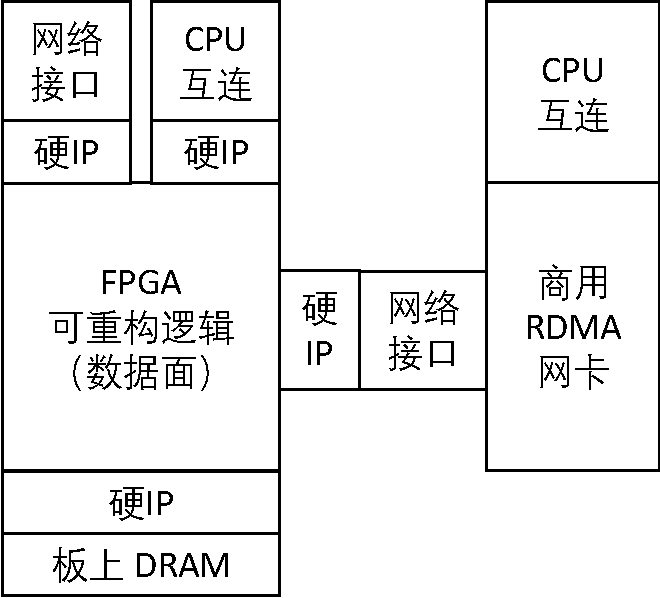
\includegraphics[width=0.4\textwidth]{figures/smartnic-current.pdf}
		\label{conclusion:fig:smartnic-current}
	}
	\hspace{0.05\textwidth}
	\subfloat[未来的片上系统。]{
		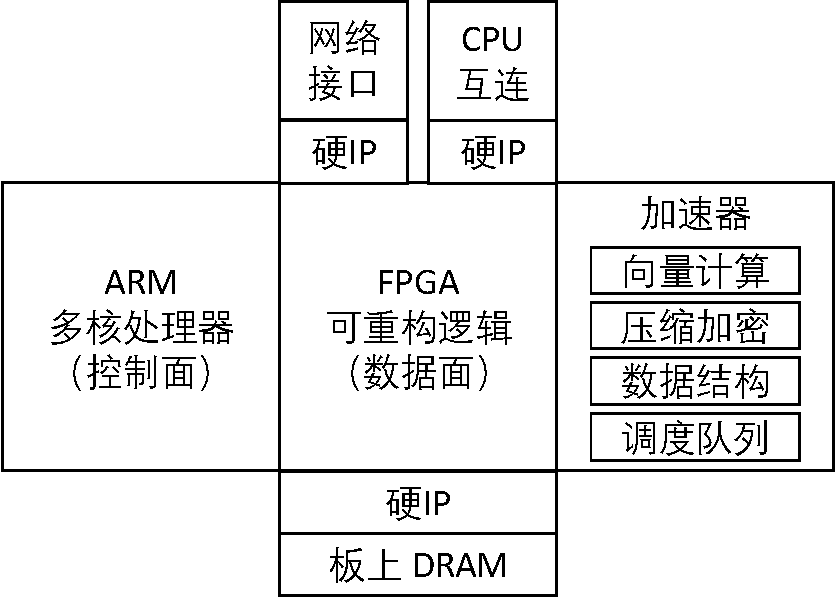
\includegraphics[width=0.5\textwidth]{figures/smartnic-soc.pdf}
		\label{conclusion:fig:smartnic-soc}
	}
	\caption{可编程网卡结构的比较。}
\end{figure}

本文使用了图 \ref{conclusion:fig:smartnic-current} 所示的 Catapult 可编程网卡。这种架构有三个局限性。
首先,现有的商用 RDMA 网卡当并发连接数较多时,性能会急剧下降 \cite{mprdma}。我们希望利用第 \ref{chapter:kvdirect} 章可扩放键值存储的技术,在 FPGA 可重构逻辑中实现 RDMA 硬件传输协议,实现高并发连接数下的高性能。这已经在第 \ref{socksdirect:sec:discussion} 节讨论过。
其次,FPGA 只适合加速数据面,控制面仍然留在主机 CPU 上。尽管它的计算量不大,但为了性能隔离,计算节点仍然需要预留少量 CPU 核用于控制面处理。第 \ref{chapter:intro} 章已经指出,即使预留一个物理 CPU 核也是相当昂贵的。为此,我们希望在可编程网卡中加入 ARM 多核处理器,用于实现控制面,从而完全消除主机 CPU 上的虚拟化开销。ARM 多核处理器的成本为数十美元,远低于一个物理 CPU 核的成本。
最后,一些类型的工作负载在 FPGA 内实现的效率不是很高,应当固化在 ASIC 加速器中。第一类是深度学习和机器学习中的向量操作、加密解密操作等计算密集型操作。例如,Intel QuickAssist 加速卡 \cite{intel-qat} 基于 ASIC 的 RSA 非对称加密比第 \ref{chapter:clicknp} 章基于 FPGA 的实现,吞吐量约高 10 倍;基于 ASIC 的 LZ77 压缩算法比本文基于 FPGA 的实现,吞吐量也高一个数量级。所用 ASIC 和 FPGA 芯片的功耗、面积和制程都接近。
第二类是常见数据结构和调度队列。基于内容寻址内存(Content-Addressable Memory,CAM)的查找表是哈希表、乱序执行引擎、缓存、模糊匹配表等多种常见数据结构的必要组件。CAM 在 ASIC 中可以用三态门实现,而在 FPGA 中实现的效率较低 \cite{wong2011comparing}。
此外,优先队列(可用移位寄存器序列或堆实现)、轮转(round-robin)调度队列、考虑依赖关系的乱序执行调度器、定时器等结构在很多应用中广泛使用,从而可以借鉴网络处理器(Network Processor)的架构,将这些通用结构硬化,让 FPGA 可重构逻辑专注于定制化计算和灵活互连。

因此,本文期待未来的可编程网卡使用如图 \ref{conclusion:fig:smartnic-soc} 所示的片上系统架构。
相比使用片外总线互连的分离组件,片上系统可以使组件间通信的带宽更高、延迟更低,更适合将计算细粒度地拆分到更适合的处理组件。
位于片上系统中心的 FPGA 不仅提供了可编程性和计算能力,也可以灵活互连和组合片上的各种计算加速器,组建定制化的内存层次结构,还可以灵活互连主机内外的各种硬件设备,组成数据中心智能互连(intelligent fabric)。

目前,业界已有基于片上系统的可编程网卡架构。例如,Xilinx 的 Versal 架构 \cite{vissers2018keynote,vissers2019versal,gaide2019xilinx} 将可重构硬件(FPGA),基于超长指令字(VLIW)的深度学习和传统机器学习加速器、数字信号处理器(DSP)和硬核(hard IP),以及多核通用处理器集成在一块芯片上,组成片上系统(System on Chip)。与传统 FPGA 相比,Versal 架构最大的区别是组成了片上系统,体现在三方面:第一,把内存控制器、PCIe 等外部接口的控制逻辑从可重构逻辑硬化成数字逻辑,减少了 FPGA 面积的开销,还能使 FPGA 实现即插即用。第二,认识到向量操作等大数据、机器学习常见计算在 FPGA 上实现的较低效率,并使用硬化的数字逻辑进行加速。第三,增加了通用处理器,可以处理复杂逻辑和控制平面,而无需绕回 CPU,这使得 Versal 片上系统可以直接驱动 Flash 存储等,组成低成本的存储服务器,而无需传统的 x86 CPU 等组件。片上系统的部件之间通过片上网络互连 \cite{swarbrick2019network,gaide2019xilinx}。Versal 架构针对数据中心服务器的多种应用加速,开发者可以把应用分解成通用处理器上的控制面、可重构硬件数据面、向量计算数据面,用合适的体系结构处理应用中的相应部分。



\subsection{开发工具链}
\label{future:toolchain}

目前,可编程网卡是主要由云计算厂商推动的新兴事物,其生态系统还不够完善。
首先,可编程网卡的编译器、调试工具、代码库等开发工具链不够灵活和易用,相关厂商的支持也不够完善。
近年来的高层次综合工具主要关注 FPGA 在计算密集型处理(如深度学习)方面的可编程性,而对通信密集型处理的关注较少。
尽管本文第 \ref{chapter:clicknp} 章的 ClickNP 在此方向做了一些努力,但与规模化的商业应用还有较大距离。

其次,目前的研究中,可编程网卡与应用程序间的任务划分是较为随意(ad-hoc)的,需要量化研究方法来确定哪些工作负载适合卸载到可编程网卡。
对于一个现有应用程序,要利用可编程网卡加速其数据面功能,需要重写大量代码:不仅需要在可编程网卡内从头实现数据面的处理逻辑,还需要修改主机 CPU 上的控制面代码以充分利用网卡的并行性和隐藏处理延迟。未来的开发工具链需要降低现有应用的二次开发成本。


\subsubsection{基于可编程网卡的 PCIe 调试工具}
\label{future:pcie-debugger}

数据中心服务器承载着越来越多的 PCIe 设备,如 GPU、NVMe SSD、网卡、加速卡和 FPGA 等。为了 PCIe 设备之间高吞吐量和低延迟的通信,GPU-Direct、NVMe over Fabrics 等技术开始流行。然而,很多 PCIe 设备只能跟 CPU 上的设备驱动程序通信,其 PCIe 寄存器和 DMA 接口很复杂,且可能没有文档。为了在 PCIe 上抓包和调试 PCIe 协议的实现,开发者往往需要昂贵的 物理层 PCIe 协议分析仪(价值 25 万美元左右)。协议分析仪需要实验室环境,难以在生产环境中动态调试。而且,协议分析仪无法修改 PCIe 数据包,也没有足够的可编程性来从大量的流量数据中发现异常或统计规律。

一个未来的方向是基于可编程网卡实现透明 PCIe 传输层协议(TLP)调试器。PCIe 调试器抓取 PCIe 设备和 CPU 之间的通信数据包。
这项工作的挑战在于,由于 PCIe 的物理拓扑和路由是固定的,不可能在 PCIe 上实施与局域网中的 ARP 类似的攻击。
然而,通过欺骗设备驱动程序,PCIe 流量可以被重定向到 PCIe 调试器。
根据请求的发起方,把 PCIe 和 CPU 之间的通信分成两类。

第一类是 CPU 发起的内存映射 I/O(MMIO)操作。这类操作中,CPU 访问 PCIe 基址寄存器(BAR)指向的内存区域。驱动程序从操作系统内核例程中获得 BAR 地址,因此可以修改该操作系统内核例程,返回 PCIe 调试器的地址,而非设备本身的地址。然后在 PCIe 调试器中建立地址映射,使 CPU 的内存映射 I/O 操作传输到 PCIe 调试器,PCIe 调试器作为代理再把请求发送给目标设备。

第二类是设备发起的 DMA 操作,用以访问主机内存。表面上看来,没有办法预知设备会访问哪个内存地址。然而,良定义的设备应当只访问驱动程序分配给该设备的地址。在 Linux 中,有两种设备驱动程序获取可 DMA 内存区域及其物理地址的方法。计划对这两种操作系统例程分别加以修改,在分配 DMA 内存区域时用 PCIe 调试器的地址取代主机内存地址,并建立 PCIe 调试器中的地址映射。这样,当设备试图 DMA 到主机内存时,事实上是 DMA 到了 PCIe 调试器,调试器随后根据映射表把数据再 DMA 到主机内存。

通过这种方法,主机驱动程序和 PCIe 设备的通信都将被 PCIe 调试器截获。基于 FPGA 的 PCIe 传输层协议调试器有足够的灵活性来修改、统计、过滤和注入数据包,进而实现对 PCIe 设备的模糊测试(fuzz testing)和压力测试。


\subsubsection{微秒级延迟隐藏}
\label{future:latency-hiding}

使用定制化硬件加速应用程序上的 CPU 处理时,原有的 CPU 软件处理逻辑被替换成了向加速器发送命令、等待加速器处理和从加速器接收结果三个步骤。在等待加速器处理期间,CPU 线程被阻塞。类似地,在分布式系统中,经常需要进行远程过程调用(RPC)并等待其他微服务或节点返回结果。传统上,开发者一般采用增加更多线程的方式隐藏加速器处理和远程过程调用延迟,也就是让操作系统在此期间切换到其他线程进行处理。然而,随着数据中心加速器性能的提高和加速任务粒度的降低,一些加速任务的执行时间只有数微秒至数十微秒。类似地,远程过程调用的网络延迟也从之前的数毫秒降低到数微秒至数十微秒。操作系统切换线程调度也需要 3 至 5 微秒,几乎与加速任务的执行时间和远程过程调用的网络延迟相当。这就意味着在等待期间切换到其他线程并不经济,让 CPU 在当前线程上等待加速任务完成可能是更好的做法。但是,这也就意味着等待期间 CPU 时间的浪费,在一定程度上影响了定制化硬件加速器节约 CPU 的效果。

一个未来研究方向是从编译的角度出发,实现应用程序的微秒级延迟隐藏。
我们有两个主要的观察:首先,应用程序可能有多个互相不依赖的硬件加速任务需要处理,因此可能挖掘出这些不依赖的加速任务,进行并发处理。
其次,很多应用程序是事件驱动的,也就是在一个永久循环里依次处理到来的事件。不同的事件处理之间可能没有依赖关系,这时就可以暂时挂起正在被处理的事件,去处理下一个不相关的事件。

这两种延迟隐藏方案的困难在于 ``依赖关系'' 的判断。在函数式编程语言中,纯函数之间的依赖关系比较容易判断。但在大多数开发者通常使用的编程语言中,内存是共享的,很多代码之间都存在依赖。例如,创建对象时需要分配内存,影响内存布局,因此从严格意义上讲,任意两个对象的创建顺序都是有依赖的。再如,两个远程过程调用是否存在依赖,往往取决于其语义。因此,问题的核心挑战是由开发者指明哪些依赖事实上是不必要的。

一种可能的方案是 ``async'' 修饰器,允许开发者指定一个函数可以被异步执行。async 函数内部可以使用 wait 调用来注册事件、释放 CPU 并在事件成立时唤醒(例如等待加速器或远程过程调用的返回)。可被异步执行的函数执行过程中不会被打断(除非调用了 wait,或有可被异步执行的子例程),因此不必担心可重入问题。每个 async 函数的执行用协程(coroutine)实现。进一步地,提出 ``async pure'' 修饰器,允许开发者指定一个函数不仅可以被异步执行,还没有任何副作用,这样就可以推测执行,即在执行的条件尚未确定时就执行之,而无需担心其产生不可撤回的副作用。

例如,把无状态计算卸载到加速器、只读的远程过程调用、打开文件是 async pure 函数。而执行写操作的远程过程调用、处理一个事件的例程是一般的 async 函数。如果 async 函数之间存在逻辑依赖关系,例如同一个用户发起的不同事件需要按顺序依次处理,那么可以为每个用户设置一个锁,在事件处理开始时加锁并在结束后解锁。锁使用 wait 调用实现,因此开销很小。

除了从编译的角度挖掘应用程序内部的并行性,另一个未来研究方向是从体系结构的角度出发,实现硬件管理的高性能上下文切换和调度 \cite{barroso2017attack}。第 \ref{smartnic-np} 节介绍的网络处理器硬件调度器可以作为有益的借鉴。

\iffalse
\subsubsection{高级语言到低级语言的翻译}
\label{future:high-to-low}

现代软件享受着摩尔定律的红利,为了开发效率,一般使用高级语言模块化编程,而编译器对软件的优化并不充分。高级语言编写的现代软件,即使与多年前基于底层语言(如 C 语言)的软件功能相似,其性能往往也相差很多。``安迪-比尔定律'' \cite{langchaozhidian} 形象地刻画了这种现象,即高性能的新型处理器(以 Intel 的 CEO 安迪代表)所增加的性能,往往被软件(以微软的创始人比尔·盖茨代表)所消耗,最终用户感受到的性能仍然是相似的。从编程框架、编译器等角度优化软件的性能也有很大的空间。David Patterson 指出,把 Python 语言重写为 C 语言,应用程序的性能可以提高 50 倍,而如果使用一系列优化,实现 1000 倍于 Python 的性能提升并不是梦想 \cite{python-to-c}。

未来的研究方向是从高级语言到低级语言的自动翻译。尽管很多高级语言是动态类型的,还有自省等高级语言特性,但对一个给定的高级语言应用程序,其输入的类型往往是相对确定的。
\fi

\subsubsection{网络应用数据面自动生成}
\label{future:p4coder}

为了提升网络应用的性能、降低 CPU 开销,数据中心引入了可编程交换机和网卡以卸载虚拟化网络功能、传输协议、键值存储、分布式一致性协议等。与通用处理器相比,可编程交换机和可编程网卡的资源较少,支持的编程模型也较为受限。
为此,开发者通常把一个网络功能分割成处理通常情况数据包的数据面和处理其余情况的控制面。数据面功能在一个数据包处理语言(如 P4)中实现,并卸载到硬件。

为网络应用卸载而编写数据包处理程序需要很多劳动。首先,即使拥有协议说明书或源代码,开发者仍然需要阅读上千页的文档或代码,进而发现哪一部分是常用功能。其次,很多实现与协议说明书之间存在细微的区别,因而开发者经常需要检查数据包的抓包记录,手工反向工程出特定于一个实现的行为。

未来的研究方向是自动学习指定网络应用的行为,从而自动生成数据面参考代码。
这样,开发者只需设计一些简单的数据面的测试用例,并运行指定的网络应用。
数据面自动生成系统将捕获输入和输出的数据包,并搜索一个数据包程序来对指定的输入测试用例产生测试得到的输出。
显然,通过测试用例并不意味着程序能在其他输入的情况下正确地泛化,因此自动生成的代码只能作为开发者的参考,开发者可以在其基础上补充特殊情况处理的细节。尽管如此,自动生成的参考程序可以帮助开发者理解协议在通常情况下的工作方式,节约大量开发时间。


一般意义上,通过例子生成程序被认为是困难的,由于巨大的搜索空间和理论上不可判定的停机问题。幸运的是,可以被卸载到硬件的数据包程序通常是比较简单的。商用可编程交换机和网卡并不支持循环和递归,因此不存在停机问题的判定难题。此外,对于每个持久化状态,每个数据包在数据面上只允许一次读写操作。而且,从数据包输入到输出的逻辑深度被硬件的流水线深度所限制。这些限制极大地降低了程序的搜索空间。
更重要的是,为了减小搜索空间,可以主动生成测试用例,以消除一些可能的搜索方向。
为了尽可能泛化测试用例,使用生成测试(generate and test)的方法来观察指定应用的行为。为了在可能的无穷多种可以生成指定输出的程序中选定一种,使用奥卡姆剃刀准则,选择具有最小描述长度的程序。当存在多个描述长度相同的程序时,系统可以生成判定性测试用例来决定正确的那个,或者报告用户。

\subsubsection{异构分布式系统的任务划分}
\label{future:work-split}

数据中心是一个异构硬件组成的分布式系统。每种硬件有一定的计算、存储和网络互连资源。不同硬件能够进行的计算类型和计算效率都不同,例如 CPU 适合控制密集型的计算,GPU 适合一般的单指令流多数据流(SIMD)类型计算,TPU 适合卷积和矩阵乘法类计算,FPGA 适合通信密集型计算。异构的硬件之间通信的能力也不同,例如 GPU 之间可以通过 NVLink 直接通信,而作为可编程网卡的 FPGA 是服务器主机与数据中心网络之间的必经之路。

给定一个计算流图及其中每个元件的高层次语言描述,一个重要的问题是如何把元件映射到异构的计算硬件。显然,仅仅考虑每个元件在各种计算硬件上的执行效率是不够的,还需要考虑元件之间通信的开销。例如,神经网络中卷积层之间的归一化运算可能在 GPU 上执行效率高于 TPU,但 GPU 和 TPU 之间数据搬移的开销可能超过在 TPU 上执行归一化运算的性能损失,因此在 TPU 上融合卷积和归一化运算可能是性能更优的。

一般地,可以将异构计算集群形式化为一张拓扑图,图中的顶点是计算设备、内存和存储设备和网络交换设备,边是节点间的数据通路。每个计算设备有若干支持的计算类型和各类型计算的带宽和延迟,而数据通路的属性包括带宽、延迟。计算流图中的每个顶点表示计算量和计算类型,每条边表示所需传输的数据量。任务划分问题的目标就是找到计算流图到异构计算集群拓扑图的一个映射,使得延迟、吞吐量满足应用的约束。

对于计算规模大的元件,还需要拆分到多个硬件上并行执行或流水线执行。一个元件的计算可能有多种拆分方式,不同拆分方式所需的通信开销不同。需要根据系统性能需求或异构硬件数量的限制计算出每个硬件上所需执行的计算量,然后根据通信和计算开销模型得到优化的元件拆分方案。



\subsection{操作系统}
\label{future:os}

分布式系统的 ``操作系统'' 包括主机上的传统操作系统和分布式系统的调度、管理、监控系统及共享的基础服务中间件。
本文研究了操作系统网络协议栈和分布式系统键值存储的优化,但操作系统中还有存储等多个子系统,分布式系统中也有消息队列等多种中间件。这些子系统和中间件显然也可以用可编程网卡加速。

此外,在传统分布式系统中,由于通信成本较高,热迁移和高可用往往需要开发者使用特定的编程框架。在拥有高性能数据中心网络的数据中心,基于可编程网卡,将可能实现通用应用程序的高效热迁移和高可用。这将让数据中心更像是一台巨大的计算机,应用可以充分利用异构的计算、存储资源,且几乎不可感知硬件故障。

\subsubsection{存储虚拟化加速}
\label{future:storage-virtualization}

云计算中的虚拟存储由本地存储和远程存储两部分构成。
远程存储则是由存储节点虚拟出的分布式存储系统,提供高可靠性、高可用性、容量可扩放性和吞吐量可扩放性,是云平台中的主要存储方式。
本地存储包括非易失性内存(Non-Volatile Memory,NVM)和 NVMe 高速闪存盘(flash storage),主要用于需要极致性能,但数据不需要高可靠性存储的分布式数据库等应用。

虚拟存储提供给客户的最基本服务是块存储(block storage),可以作为块设备(block device)挂载到虚拟机作为磁盘使用。
云服务还提供了对象存储(object storage)、文件存储(file storage)等存储服务。
这类服务大多提供类似键-值(key-value)映射的抽象,即用户指定键,读取(GET)或写入(PUT)相应的值。
键-值存储作为一种基础数据结构,可以分为持久化存储、临时存储;根据是否需要复制和容灾,是否支持事务(transaction),提供强一致性或最终一致性 \cite{anna},是否支持范围索引、二级索引、内容索引等,可以组合出形形色色的存储系统,满足不同应用的需求。

虚拟存储系统的两个基本逻辑概念是客户端和服务器。
如图 \ref{background:fig:storage_arch} 所示,客户端是云存储服务的使用者,如云上承载客户虚拟机的计算节点;服务器提供块存储、对象存储、文件存储等抽象,把逻辑存储的读写请求映射到物理存储介质的读写请求。
多个客户端可能共享同一个虚拟存储,例如分布式数据处理系统中的多个计算节点可能需要访问共享的原始数据和配置参数,数据处理的中间结果也可以通过存储来传递。
同一个虚拟存储可能对应多个存储服务器,用于实现存储的容量可扩放性、吞吐量可扩放性、容错和高可用。


\begin{figure}[htbp]
	\centering
	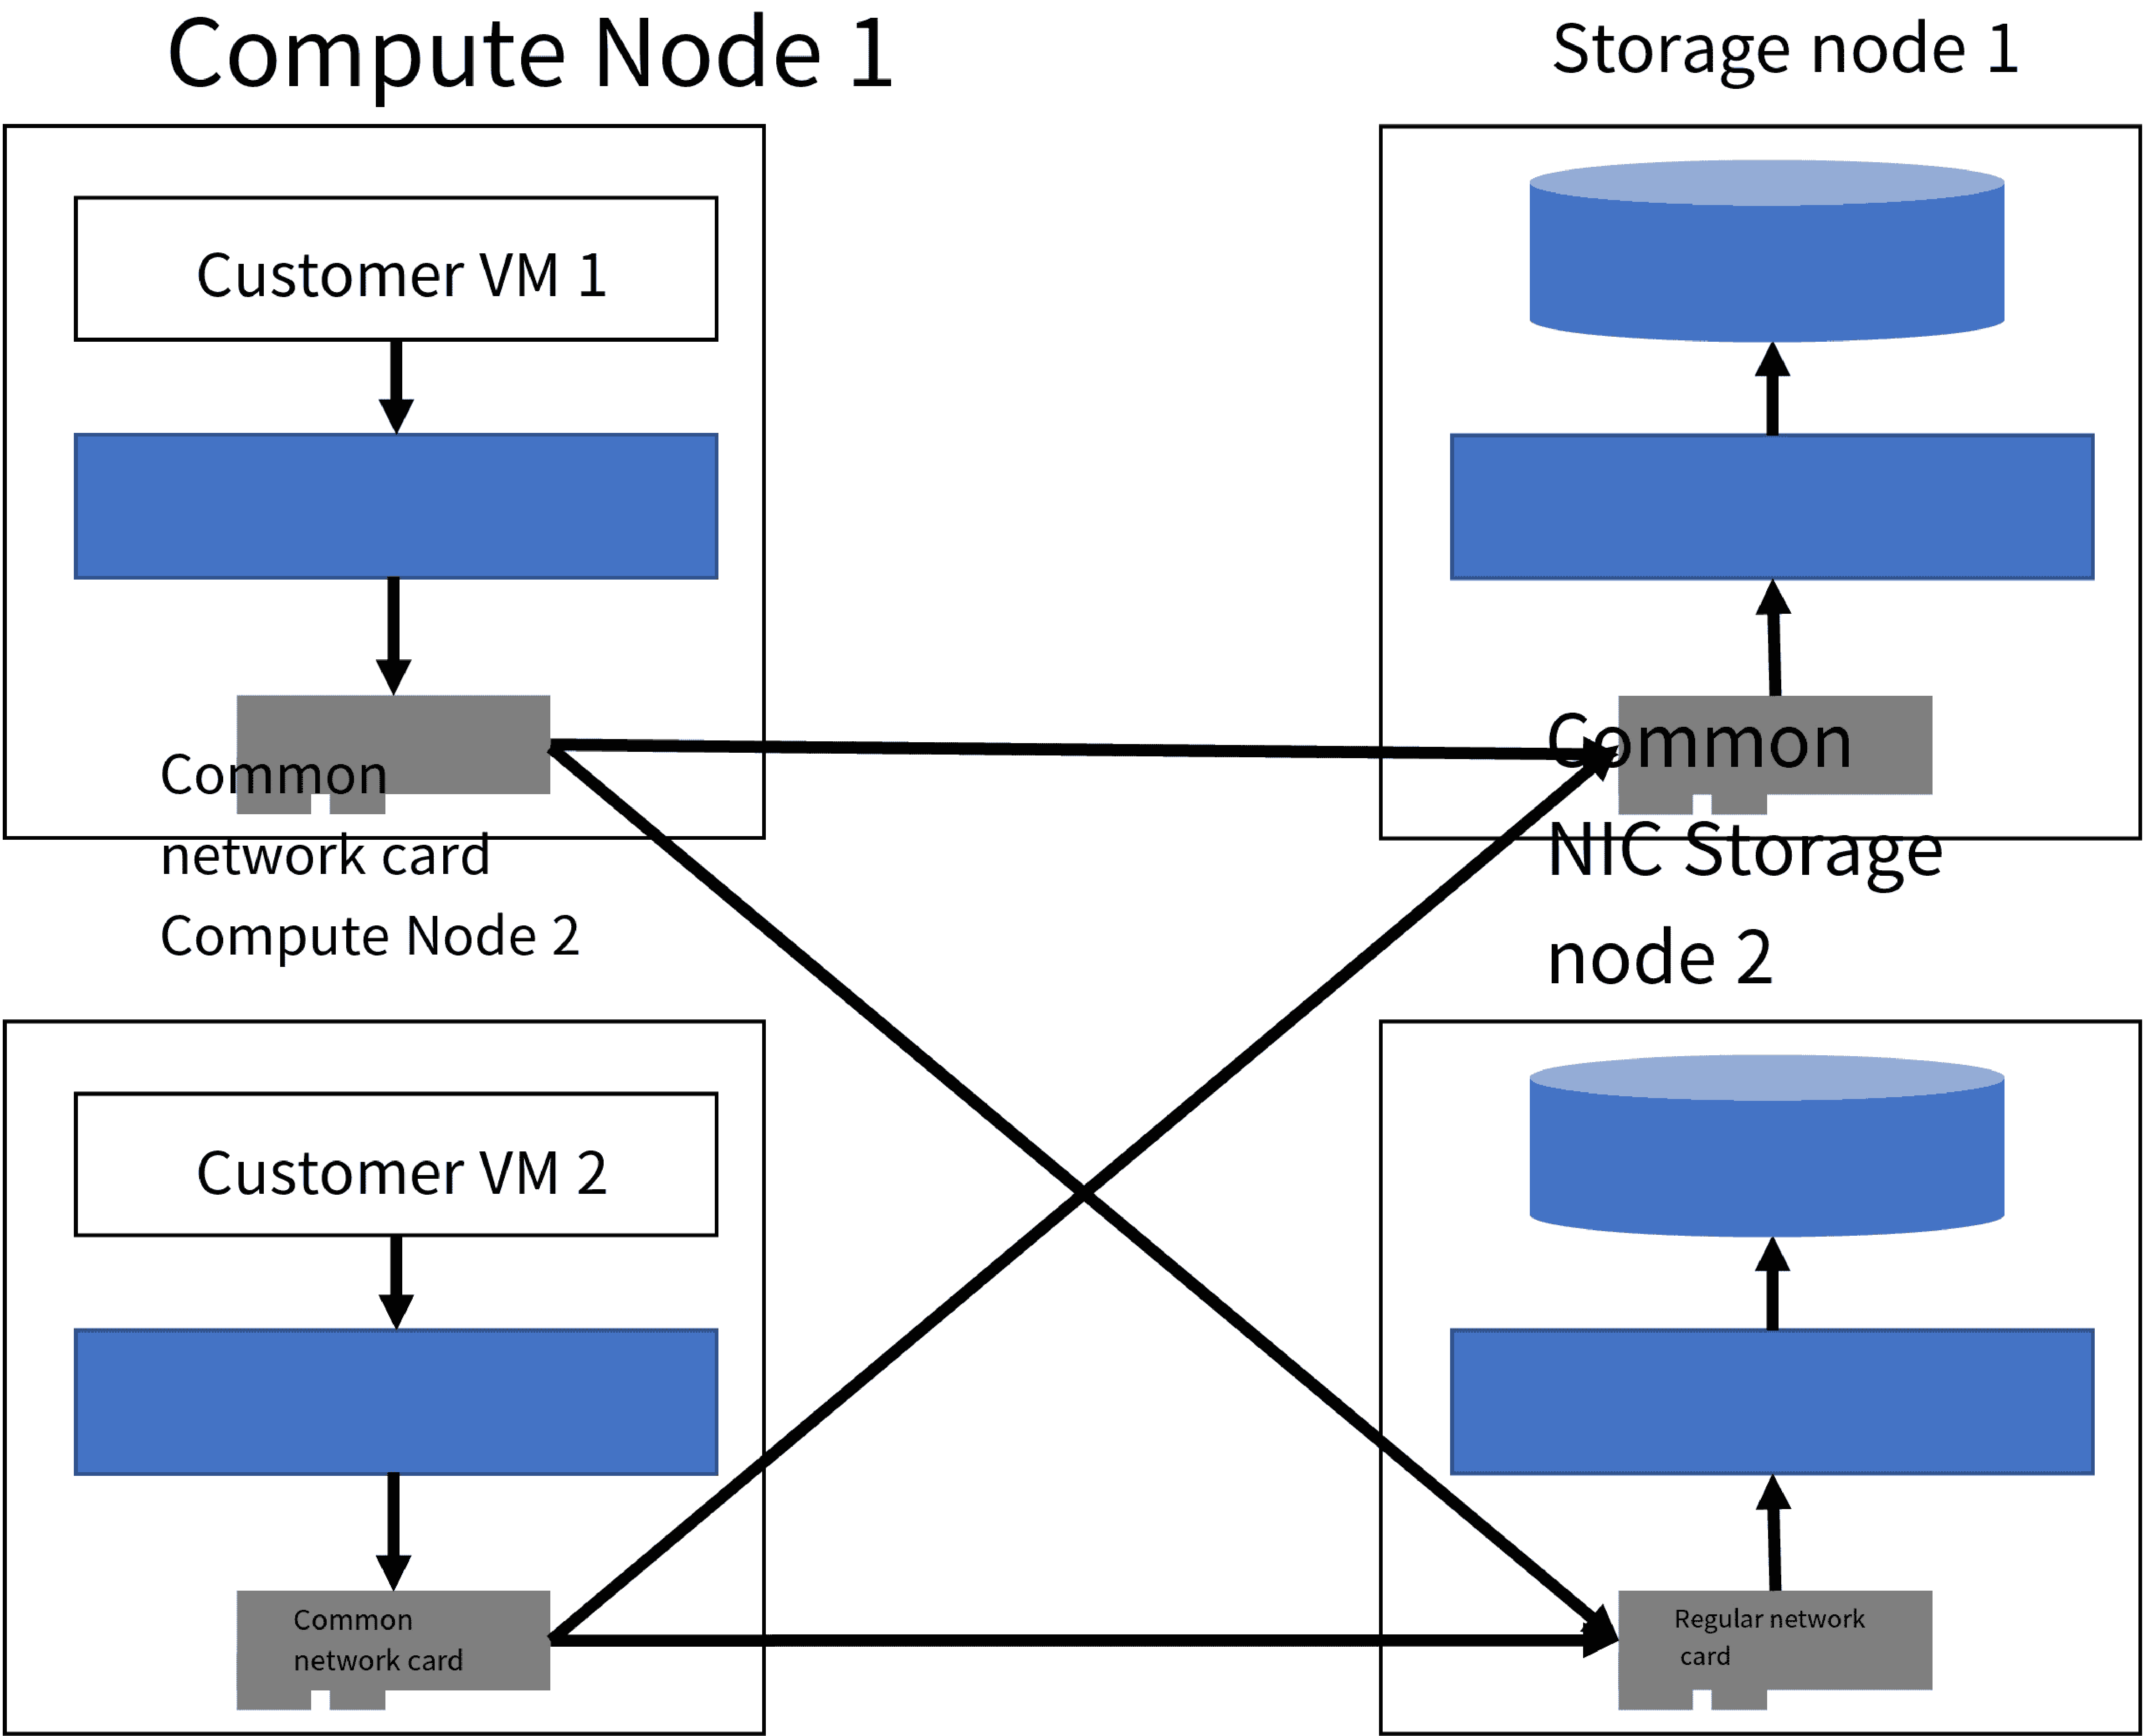
\includegraphics[width=0.6\textwidth]{figures/storage_arch.pdf}
	\caption{数据中心云存储的简要架构。}
	\label{background:fig:storage_arch}
\end{figure}


上述存储服务器的结构是较为简化的,事实上往往分为多个层次。
例如,微软 Azure 的云存储服务分为前端节点、中间节点和后端节点 \cite{calder2011windows}。
前端节点负责解析和验证请求,并根据数据分片映射表(例如键的哈希值),分发到数据所在分片的中间节点。中间节点负责实现请求的处理和存储数据结构的处理,把用户的请求映射成一系列存储读写操作,分发给对应的后端节点。后端节点负责实现数据的复制(replication)以及在物理介质上的存储。

在软件处理之外,数据中心存储还有显著的网络开销。
在数据中心中,由于存储服务器需要安装较大容量的存储介质,存储节点的硬件配置一般与计算节点是不同的。此外,计算节点上由于运行客户的虚拟机,虚拟机监控器软件经常需要升级以增加新功能和修补安全漏洞,因此计算节点的稳定性通常比存储节点低。为了保证存储的高可用性,存储节点与计算节点通常是分离在不同物理主机上的。因此,计算节点上的存储客户端通常需要把数据从存储服务器通过网络搬运过来。
也就是说,客户虚拟机的每个 I/O 请求都需要被虚拟机监控器捕获,然后从计算节点上虚拟机监控器内的存储客户端软件出发,依次经过存储服务器的前端、中间和后端节点的处理,才能到达存储介质。
为了保证数据的安全性,物理存储介质上的数据一般需要加密存储。为了节约存储空间,降低单位存储容量的存储介质成本,很多云厂商还会对存储的内容进行压缩。压缩和加密一般在存储服务器上进行,属于计算密集型操作。例如,根据实验,在 LZ77 较好的压缩率下,一个服务器 CPU 核心每秒通常只能压缩 100 MB 的数据;对 1 KB 的块,AES 加密和 SHA-256 签名每秒也只能处理 100 MB 的数据。

由于软件处理和网络传输的开销,云计算平台上块存储的延迟一般为 0.5 至 1 毫秒,对象存储的延迟一般为 1 至 10 毫秒 \cite{jonas2019cloud},远高于物理存储介质的延迟(如 SSD 的延迟一般为 0.1 毫秒)。
此外,云存储的吞吐量也低于相应的物理存储介质,例如 SSD 云盘最高的吞吐量为 50 K 次 I/O 每秒,而单块数据中心级 SSD 的吞吐量就已达数百 K 次 I/O 每秒 \cite{jonas2019cloud}。
为了充分利用最新的数据中心存储硬件的性能,云存储服务需要全栈优化。
例如,很多数据中心在存储协议栈的网络传输方面,已经使用 RDMA 协议降低了网络协议栈的 CPU 开销和延迟 \cite{guo2016rdma}。
一些数据中心还通过改进云存储的协议栈,把客户端、服务器前端、中间、后端节点的功能进行适当的整合,减少层次 \cite{nitro-blog}。
HyperLoop \cite{kim2018hyperloop} 利用 RDMA 网卡和非易失性内存(NVM)降低了存储写入事务的延迟。

\subsubsection{远程过程调用和消息队列加速}
\label{future:rpc}

分布式系统中的消息传递通常采用远程过程调用(RPC)或消息队列(message queue)模型,或者两者的结合。在 RPC 模型中,服务器端注册一个过程(procedure)来响应客户端的 RPC 请求。在消息队列模型中,生产者将消息广播或者分发到若干消费者。为了实现生产者与消费者的解耦以及消息的缓冲和可靠投递,消息队列模型往往引入一个经纪人(broker)服务,如 Kafka \cite{kreps2011kafka}。在编程接口方面,分布式应用程序通常使用 RPC 库和消息队列中间件(middleware),这些库和中间件则依赖操作系统的套接字(socket)接口来发送和接收消息。
本文研究了操作系统套接字接口的加速,但没有考虑更上层的 RPC 和消息队列中间件。谷歌的研究 \cite{barroso2017attack} 表明,这些消息中间件经常增加数十微秒的延迟,占到整个端到端网络延迟的很大一部分。
为了降低分布式系统的端到端消息传递延迟,有必要利用可编程网卡等硬件和用户态库等软件,实现高性能的 RPC 和消息队列。
一种方案是在本文第 \ref{chapter:socksdirect} 章的用户态套接字系统基础上,实现 RPC 和消息队列等高层抽象;另一种方案是打破传统网络协议栈边界的全栈优化,如最近的 eRPC \cite{kalia2018datacenter} 是这方面很有意义的探索。
对于消息队列等比较简单的应用,甚至可以探索在可编程网卡中实现,绕过主机CPU。

\subsubsection{基于微内核的用户态操作系统}
\label{future:user-space-os}

本文第 \ref{chapter:socksdirect} 章提出了一个用户态网络协议栈 SocksDirect。第 \ref{chapter:socksdirect} 章的技术可以用于加速操作系统的更多抽象。

在网络协议栈之外,操作系统的存储协议栈也有较高的开销。
Linux 存储协议栈逻辑上由五层构成。首先,是与网络协议栈类似的虚拟文件系统层,提供基于文件描述符的 API。
其次,文件系统层实现文件系统的抽象,提供文件的路径查找、权限管理、空间分配等功能。
第三,缓存缓冲层与 Linux 的内存管理机制紧密结合,负责管理读缓存和写缓冲,以及页面换入换出机制。
第四,块设备层把存储设备抽象为若干个 ``块''(block),实现块访问的合并、排序等。
第五,在设备驱动层,存储介质驱动程序与硬件通信以读取和写入硬盘块。
在存储协议栈中,虚拟文件系统层也是开销的重要来源。对数据库等很多使用直接 I/O 的应用,文件系统、缓存缓冲层是不必要的。
与网络协议栈类似,存储协议栈中也存在多次数据拷贝。对于很多应用,还存在存储和网络协议栈间的拷贝。基于页面重映射的零拷贝技术可以用于网络和存储协议栈,实现每份数据在物理内存中只有一份拷贝,在协议栈间复制的仅是虚拟内存的映射关系。

本文第 \ref{chapter:socksdirect} 章的技术有更广阔的应用前景:基于微内核的用户态操作系统。
操作系统主要包括三方面的功能:资源虚拟化、进程间通信和高层次抽象。
第 \ref{chapter:socksdirect} 章实现了网络资源的虚拟化和进程间的消息传递,提供了套接字的高层次抽象。
用户态存储协议栈可以实现存储资源的虚拟化和文件系统的高层次抽象。
其余的操作系统功能还包括计算资源虚拟化(即进程调度)和进程间同步(如锁和信号量)。
这些功能可以在用户态守护进程中实现,也可以在可编程网卡中实现。
将传统操作系统的功能被移动到用户态和可编程网卡后,就可以采用微内核,并保持与现有应用程序的兼容性。

基于微内核的操作系统不仅具有更高的性能,还便于实现通用分布式应用的高可用性,这将是下一小节讨论的主题。

\subsubsection{通用分布式应用的高可用性}
\label{future:ftlinux}

硬件故障和操作系统崩溃都可能导致分布式应用的部分节点出错。
分布式应用的高可用性是很重要的。
很多现有的请求处理和批量处理系统可以简化分布式应用的容错编程。
这些程序通常需要程序员把组昂泰显式地从计算中分离,并把状态存储到一个容错存储系统中。
然而,很多现有应用(如 Node.js,Memcached 和 Tensorflow 中的 Python 逻辑)并不原生支持容错。此外,容错编程框架通常比不容错的版本性能低。
我们希望解决通用分布式应用程序的透明和高效容错的挑战。
具体来说,挑战分为进程迁移、确定性重放和分布式快照三个方面。

首先,在不同层次上的容错存在着权衡。
在体系结构层次上的容错需要定制化硬件。
在虚拟机层次上的容错机制认为所有网络通信都是双向的(因为有数据传输和 ACK 确认报文),并且不能发现诸如进程间通信的高层次语义。
系统调用层次上的容错需要对操作系统内核的修改以实现进程迁移,例如,从源主机把进程状态提取出来,并注入到目的主机里。
Linux 系统中的进程迁移较为复杂,因为来自不同进程的状态混杂在一个宏内核中。
而 Unikernel 方法不能支持很多现有的进程间通信机制。
为此,未来的研究工作可以借鉴本文第 \ref{chapter:socksdirect} 章的 SocksDirect 架构,设计一个分布式的用户态运行库操作系统,与现有 Linux 应用程序编程接口兼容。
进程的内存快照同时获得了运行库和应用程序的状态,同时保留了高层语义,便于优化。

第二,状态机复制(State Machine Replication,SMR)和快照重放(snapshot replay)是实现容错的两种主要方法。 SMR 至少需要两台主机才能执行完全相同的应用程序,从而引入 CPU 开销。基于快照的系统通常在两个相邻快照之间的间隔期间缓冲应用程序的输出,因为当主机发生故障时,系统无法保证自上次快照以来的确定性执行。这种所谓的输出提交(output commit)问题为透明容错系统引入了显着的请求服务延迟。或者,记录应用程序的所有非确定性事件仍然会产生很大的开销。未来的研究方向是采用根据其最近的执行历史来预测应用程序的非确定性事件。如果预测正确,则应用程序继续。否则,等待很短的时间来实现预测,因为许多不确定性源于微小的时间波动。这样,系统只需在等待超时的时候记录错误预测的事件,减少记录开销。

第三,透明容错机制需要在不暂停整个系统的情况下拍摄分布式应用程序的快照。一致的快照算法要求所有主机以相同的速度拍摄快照,并在任何主机发生故障时同时回滚。这种全局同步的行为与容错的目标相矛盾,容错需要系统在主机发生故障时继续提供对延迟敏感的请求。如何异步地对分布式系统生成一致的快照是未来的研究方向。


\subsubsection{基于热迁移的数据中心资源打包}
\label{future:resource-packing}

现代数据中心的资源利用率较低,有较大的优化空间。例如,数据中心内大部分物理服务器的平均使用率只有大约 10\% 到 15\%,但是闲置时的功耗却与使用率最高时相差仅 30\% \cite{barroso2018datacenter}。一方面,服务器和硬件的节能设计可以改进,以在使用率较低甚至闲置时尽量降低功耗。另一方面,云计算的一项优势就是支持热迁移,理论上可以在客户几乎不感知的情况下,根据虚拟机的计算、内存、存储、网络等需求,把需求互补的虚拟机打包安排在一台物理服务器主机上,从而最大化利用物理服务器的各种硬件资源。目前,热迁移对客户服务会造成一段时间的性能下降甚至中断,因此在云计算中的利用还不够广泛。

热迁移的主要难点在于生成一致的虚拟机状态快照。在异构硬件组成的数据中心,虚拟机的状态不仅包括其 CPU、内存和本地存储的状态,还包括 GPU、网卡等硬件的状态。这些硬件往往没有提供高效的快照和恢复功能,从而只能在新物理节点上重新加载硬件驱动程序、初始化硬件内部状态,带来较高的延迟。第 \ref{chapter:clicknp} 章的 ClickNP 框架可以实现网络元件内部状态的快照和迁移,因此采用 ClickNP 框架编写的可编程网卡可以高效热迁移。GPU-Direct RDMA 等技术可以实现 GPU 内部存储的高效传输。对于本地存储,可以利用存储解聚的思想,不必等待数据迁移完成,而可以在迁移过程中把新节点上虚拟机的访问请求重定向到原有存储。

\subsubsection{端云融合的分布式操作系统}
\label{future:distributed-linux}

智能终端(如智能手机和 PC)和云(数据中心)是目前最重要的两类计算和存储设备。端和云的计算和存储能力都在快速增长,且随着 5G 技术的发展,端云之间的通信成本将大幅降低,带宽和延迟也将显著改善。因此,端云融合将成为重要的趋势。一方面,端上的应用将可以更细粒度地调用云上的服务、访问云上的数据;另一方面,云上用于高性能通信和计算的技术也会逐渐应用到端上。例如,通过在端上部署可编程网卡,可以为 5G 网络通信降低功耗开销,消除性能瓶颈;可以提高访问 Flash 存储的性能,本文第 \ref{chapter:socksdirect} 章的高性能用户态套接字技术也可以在端上得到应用。

当端上的应用需要较大的算力、存储空间,或需要长时间地运行任务时,往往需要卸载到云上处理。无服务器计算(serverless computing)简化了云上的任务调度,但仍然需要开发者在端云间进行任务划分,并设计远程过程调用(RPC)接口。
本文期待未来的工作提出端云融合的分布式操作系统。在端云融合操作系统中,应用在端和云上有相同的开发环境和运行环境。应用可以直接访问云上的计算、存储和网络资源,而无需关注其本身是运行在端上还是云上。
一个应用由若干进程组成,每个进程运行在端或云上的一个计算设备上,并允许动态迁移计算设备;不同进程可以运行在不同的计算设备上,进程间可通过分布式操作系统提供的基于消息传递或共享数据结构存储的中间件来通信。
为了支持网络测量、爬虫等需要分布在不同地理位置的应用、由于隐私保护法律需要限制数据的处理和存储区域的应用以及为了开发者提升数据局部性,应用可以指定进程可以运行、数据可以存储的计算设备集合。
分布式操作系统的主要挑战是将进程内存状态和共享数据结构存储中的数据在端云的计算节点之间合理复制和缓存,以提高数据局部性,降低通信延迟。

作为一个示例,用户在 PC 终端上启动一个并行编译任务,传统上该任务的并行度将受限于 PC 上的 CPU 核数,且消耗 PC 较多的电池能量。在端云融合的分布式系统中,如果传输源文件及编译结果的通信代价低于计算的代价(或者待编译文件在云上已经有副本),该任务将被分发到云端的多台服务器上,编译任务的不同子进程将运行在不同服务器的 CPU 核上,并行度理论上仅受限于编译任务可并行执行的最大子进程数以及端云之间的通信带宽。对于编译结束后的链接过程,分布式操作系统不必将编译结果传回 PC 终端再上传到云上做链接,而是可以直接在云端的计算节点间通信,完成链接操作,最后 PC 终端只需要下载链接后的最终二进制。甚至,如果该二进制与用户的交互并不频繁,延迟也不敏感,分布式操作系统可以不传输该二进制到端上,而是在该二进制执行时只传输用户与计算节点间的交互,相当于在操作远程的服务器。

值得讨论的是分布式操作系统的抽象层次。如果在 Linux 操作系统的层次上抽象,兼容性将最好,可以实现现有并行程序的自动分布式处理。但 Linux 系统调用的抽象层次较低,如果开发者不显式提供更多信息,较难预测应用未来访问的资源,对一些类型的应用将性能不佳。实现分布式 Linux 操作系统的一种可能的方式是远程系统调用,即对每个迁移到远程的进程,在本地保留一个影子进程;捕获远程系统上的系统调用,发送到本地影子进程并实际调用,并将系统调用的结果发送到远程系统。应用进程需要等待远程系统调用返回,即系统调用的延迟大大增加,因此该实现方案的性能可能不佳。


\subsection{系统创新}
\label{future:system}


把整个世界看作一台大型计算机是微软 CEO 萨提亚·纳德拉的愿景,也是很多系统研究者的梦想。云计算的成功使数据中心吸纳了人类世界大部分的计算和存储,而数据中心可以看作是由计算、内存、存储和网络及互连四部分组成的一台大规模计算机。英伟达 CEO 黄仁勋 \cite{nvidia-datacenter}、谷歌工程副总裁 Luiz Barroso \cite{barroso2018datacenter} 等已经将数据中心看作一台大规模计算机。系统创新就是从全局的角度考虑各种软硬件组件如何高效而可靠地协同工作,以及给用户提供怎样的抽象。


\subsubsection{基于可编程网卡的内存解聚与二层内存}
\label{future:second-tier-memory}

内存解聚(Memory Disaggregation)指的是计算机的 CPU 可以自由而透明地高效共享远程计算机的内存,这样可以大大增加内存的利用率,降低云计算平台的成本。
尽管目前数据中心网络的性能远低于 CPU 访问主机内存的性能,幸运的是,利用内存访问的局部性,如果一部分热数据仍在本地,剩余的数据通过远程访问,则远程内存的带宽和延迟要求能比本地内存大大降低。加州大学伯克利分校的研究指出,要把内存解聚后的系统性能与全部使用本地内存的差距控制在 5\% 以内,带宽需要达到40 Gbps,端到端往返延迟需要不超过3 至 5微秒,这是目前的数据中心网络可以达到的。

非易失性内存(Non-Volatile Memory,NVM)是内存和存储领域的研究热点。相比传统的NAND Flash,非易失性内存的存取速度要快得多。虽然它们短期内还不能完全取代 DRAM,但至少希望能够在不久的将来会代替一部分普通内存。
非易失性内存相比DRAM有价格低,容量大,功耗小,断电可以保持数据的优点,但同时又有存取速度慢,写入周期有限等限制。
非易失性内存作为 DRAM 和 NAND Flash 之间的存储层级,既可以用来扩充 DRAM 内存的容量,又可以作为快速的持久化存储。
如何有效地利用非易失性内存目前是一个重要研究方向。

内存解聚和非易失性内存构成了二级内存(second-tier memory),即比 DRAM 慢但容量更大的内存 \cite{dulloor2016data}。为了扩充内存容量并尽量减少对应用性能的影响,二级内存系统需要把热数据放在本地 DRAM 中,把冷数据放在解聚的远程内存或非易失性内存中。
目前的大多数内存解聚系统(如 Infiniswap \cite{gu2017efficient})和二级内存系统(如 Thermostat \cite{agarwal2017thermostat})采用页面换入换出的方式。首先,页面换入换出需要经过操作系统内核,每换入一个页面需要增加约 2.5 微秒的内核开销,而允许的端到端访问延迟只有 3 至 5 微秒。其次,解聚到远程存储的内存一般是冷数据,这些数据的访问粒度可能小于一般为 4 KB 的页面大小,因此传输一整个页面不仅浪费网络带宽,也增加了延迟。最后,页面换入换出的决策在软件上进行,难以准确统计每个页面的访问频率。

未来的研究方向是基于可编程网卡的内存解聚和二级内存。通过使用直接内存映射取代页面换入换出,避免了操作系统内核的开销,也把内存访问的粒度从 4 KB 的页面降低到 64 字节的缓存行。本地与远程内存仍然是以页面为单位,依靠页表维护映射关系。可编程网卡可以统计每个页面的远程内存访问,从而及时把热数据迁移到本地内存,避免长期影响性能。

基于现有 CPU 和 PCIe 体系结构实现基于直接内存映射的内存解聚存在一系列技术挑战。幸运的是,CPU 厂商已经意识到了同样的问题。我们期待随着 CCIX 等主机内互连协议的实现,直接内存映射的可编程网卡与 CPU 之间将达到更好的吞吐量和延迟,并且直接内存映射区域可以像主机内存一样运行所有指令。


\subsubsection{基于数据中心网络的可扩放全序通信}
\label{future:system-network-codesign}



传统数据中心网络中的延迟是任意的,从而消息不能保证按照一致的顺序被投递。例如,分布式数据库的多个分片向多个副本发送日志。每个副本可能以不同的顺序收到各个分片的日志。如果不加特殊处理,这种不一致的顺序可能破坏数据一致性。解决这个问题的方案经常引入同步开销,并使分布式系统的设计复杂化。

全序通信提供了一种抽象,保证不同的接收端按照一致的顺序处理来自发送端的消息。
全序(但不可靠)地传递一组消息可以简化和加速很多分布式应用,例如减少多版本并发控制(MVCC)协议中的冲突,加速分布式共识协议,实现无中心瓶颈的可扩放日志复制(replication),提早检测 TCP 尾丢包,降低散播-汇聚(scatter-gather)模式远程过程调用(RPC)的尾延迟。
例如,近年来,通过提高数据中心内传输的有序性,分布式共识协议(consensus protocol)和分布式事务的性能得到了极大的提升。
快速 Paxos~\cite{lamport2006fast,kemme1999processing,moraru2013there,pedone1998optimistic} 协议采用尽力而为的方法提高传输的有序性。
Speculative Paxos~\cite{ports2015designing} 和 NOPaxos~\cite{li2016just} 利用可编程交换机作为中心化的序列号发生器或序列化点。
NetPaxos \cite{dang2015netpaxos,dang2016paxos} 和 \cite{dang2016network} 把传统 Paxos 协议放在网络交换机中实现。
Eris~\cite{eris} 提出使用网络交换机作为序列号发生器,在网络中实现并发控制,实现了快速事务处理。
HotOS '19 上的工作 \cite{synchronous-datacenter} 提出构建同步,即网络延迟固定的数据中心网络,可以简化分布式系统的设计。

自从分布式系统研究的兴起,全序广播和多播问题就吸引了大量的研究。然而,现有方案受限于可扩放性或效率。一类研究工作利用逻辑上中心化的协调,例如中心化的序列号发生器,或者在发送端或接收端之间传递的令牌。
近年来分布式系统和数据中心网络共同设计的研究工作属于此类。
然而,这些中心化的方案难以扩放。
另一类研究工作用完全分布式的协调,例如在接收端开始处理消息之前交换时间戳。这导致额外的网络通信开销和延迟,降低系统效率。此外,多播的语义还有一个限制,即所有接收者必须收到相同的消息。

相比全序多播,全序消息散播(Total-Order Message Scattering,TOMS)原语的应用范围更广。
消息散射是一种一个主机同时发送一组(可能不同的)消息给多个主机的通信原语。消息散射在分布式系统中很常见。例如在分布式存储中,一个客户端把元数据写到一个存储站点,把数据写到另一个存储站点;与此同时,另一个客户端并发地读取它们。元数据和数据间的一致性要求这些操作被原子地散射到两个存储站点。
全序消息散播在数据中心网络中一对多地散射一组消息,并保持可线性化的顺序,每条消息至多被投递一次。

为了支持更好的可扩放性,也为了加速除分布式事务外的更多分布式应用,基于数据中心网络的可扩放全序通信是一个有趣的研究方向。
在数据中心环境中,网络拓扑是规则的,交换机一般有较好的可编程性。
全序消息散播把工作分配给每个交换机和终端服务器,从而实现了高可扩放性。
核心设计原则是把顺序信息的处理与消息转发分离开来。
为了得到顺序信息,利用可编程交换机,在网络中汇聚顺序信息,这形成了系统的 ``控制面''。
在 ``数据面'' 上,全序消息散播像往常一样转发消息,并在接收端缓冲并重排收到的消息。
发送端给散播的每组消息打上递增的时间戳,而接收端需要按照时间戳的顺序向应用投递消息。
控制面的顺序信息为接收端提供了 ``在此之后收到的消息都晚于某个时间戳'' 的屏障(barrier),使其可以按照时间戳顺序投递消息。

本研究的初步工作已经由合作者左格非发表在 ACM SOSP 2017 学生研究竞赛(SRC)上 \cite{toms}。

全序通信研究的一大难点是可靠性。如果需要在有丢包和节点故障的网络中保证可靠全序通信,这至少与分布式共识(consensus)问题一样困难,将需要较为复杂的容错与故障恢复机制,且局部的故障很容易影响全局的通信效率。如果不保证通信的可靠性,而是只保证收到的数据包有序,则应用范围将大大缩小,必须与其他传统方法结合才能保证分布式系统的正确性,但可以大大减少乱序情况而提高效率。

分布式事务的其他方面也可以受益于与数据中心网络的协同设计。
Hyperloop~\cite{kim2018hyperloop} 在存储节点上利用可编程网卡把写操作写入非易失性内存中的缓冲区,并立即向计算节点回复确认消息,再由存储节点上的软件异步处理非易失性内存中的写操作。这消除了写操作等待存储节点软件处理的延迟。
Google Spanner~\cite{corbett2013spanner} 利用全球同步的 GPS 时钟实现了跨地理区域复制的高性能数据库。


\subsubsection{结合在线事务、批量和流式处理的数据库}
\label{future:reactdb}

现代大数据处理主要有在线事务处理(OLTP)、批量处理(batch processing)和流式处理(stream processing)三种范式。在线事务处理用于需要较快响应时间、较强一致性的事务,一般每个事务只涉及数据集的一小部分,且更新操作频繁。批量处理主要用于离线数据分析,其特点是数据量和计算量都很大。流式处理适用于需要高实时性的分析任务,可以针对数据的改变增量地更新状态并输出结果。

传统上,大数据处理系统一般使用 lambda 架构,即在线事务处理作为批量处理和流式处理的数据源,其产生的数据更新分别同步到批量处理部分和流式处理部分。批量处理部分定期重新计算结果,而流式处理部分根据上次的批量处理结果和流式输入的更新数据来持续更新输出。最后,批量处理部分和流式处理部分的输出被合并起来,输出给用户。首先,lambda 架构需要数据分析人员显式把数据分成在线、批量和流式三部分,分别编写处理程序,并将结果归并,开发较复杂,且容易导致不一致。其次,lambda 架构中的流式处理可能依赖上次批量处理的结果,批量处理延迟可能导致结果的不准确性,而这种延迟在性能上不一定必要。

近年来,在同一个数据库中结合在线事务处理(OLTP)和离线数据分析处理(OLAP)事务的 HTAP(Hybrid Tranactional and Analytical Processing)数据库开始流行。HTAP 数据库解决了从在线事务处理到批量处理分析的延迟问题,但仍然不支持流式处理。用户需要显式重新运行查询来获取更新后的批量处理结果,而且处理是基于查询开始时的数据库状态,不能反映数据库的实时状态。学术界提出的 DBToaster 等响应式数据库结合了在线事务处理和流式处理,但所有中间结果都被缓存和增量处理,其中的开销是很大的。例如,一些类型的批量处理难以增量更新,性能上比较合理的做法是允许一定的数据更新延迟。

未来的研究方向是同时高效支持在线事务处理、离线数据分析和流式处理的响应式数据库系统。响应式体现在三方面。首先,每个存储过程事务都对其他并行事务的更新操作是响应式的。基本表的更新被同步到运行着的离线数据分析和流式处理事务。这些正在运行的事务保存适当的中间状态,并增量更新之。因此,每个事务都天然地在事务完成时间被序列化,也就是存储过程事务的查询结果反映了数据库的实时状态。流式处理事务则被认为是持续运行的,能够把数据库增量更新对查询结果的改变实时报告给用户。

其次,事务处理的计算流图的 ``推'' 和 ``拉'' 是响应式的。在数据库内部的计算流图中,传统数据库的每个算子都是 ``拉'' 模式的,也就是每次用户需要查询结果时,就重新执行计算流图;而流式处理和响应式数据库中,每个算子都是 ``推'' 模式的,也就是每次基础表的数据有更新时,都会更新并保存所有中间算子的结果,直到更新最终查询结果,不论用户是否需要实时的更新。根据用户对更新时效的需求,数据库动态调整计算流图中每个算子的 ``推'' 和 ``拉'' 模式,以及 ``推'' 的频率。

最后,物理数据存储结构与索引是响应于数据访问模式的。
把基础表的数据更新日志作为数据源,而基于行、列的数据存储结构都是缓存,为点查询和分析性查询分别优化。索引也被认为是缓存。视图和分析型查询的中间结果也可能被缓存下来。
数据库需要根据数据的访问模式来调整缓存与否的选择,因为缓存可以加速读操作,但对写操作增加了负担。

\iffalse
\subsection{基于可编程交换机的全序消息散播}


在有任意延迟的网络中,消息不能保证按照一致的顺序被投递。例如,分布式数据库的多个分片向多个副本发送日志。每个副本可能以不同的顺序收到各个分片的日志。如果不加特殊处理,这种不一致的顺序可能破坏数据一致性。解决这个问题的方案经常引入同步开销,并使分布式系统的设计复杂化。

全序通信提供了一种抽象,保证不同的接收端按照一致的顺序处理来自发送端的消息。
全序(但不可靠)地传递一组消息可以简化和加速很多分布式应用,例如减少多版本并发控制(MVCC)协议中的冲突,加速分布式共识协议,实现无中心瓶颈的可扩放日志复制(replication),提早检测 TCP 尾丢包,降低散播-汇聚(scatter-gather)模式远程过程调用(RPC)的尾延迟。

自从分布式系统研究的兴起,全序广播和多播问题就吸引了大量的研究。然而,现有方案受限于可扩放性或效率。一类研究工作利用逻辑上中心化的协调,例如中心化的序列号发生器,或者在发送端或接收端之间传递的令牌。因此,这样的系统难以扩放。另一类研究工作用完全分布式的协调,例如在接收端开始处理消息之前交换时间戳。这导致额外的网络通信开销和延迟,降低系统效率。此外,多播的语义还有一个限制,即所有接收者必须收到相同的消息。

我们提出全序消息散播(Total-Order Message Scattering,TOMS)原语。
TOMS 把多播原语泛化到消息散射原语。消息散射是一种一个主机同时发送一组(可能不同的)消息给多个主机的通信原语。消息散射在分布式系统中很常见。例如在分布式存储中,一个客户端把元数据写到一个存储站点,把数据写到另一个存储站点;与此同时,另一个客户端并发地读取它们。元数据和数据间的一致性要求这些操作被原子地散射到两个存储站点。
全序消息散播在数据中心网络中一对多地散射一组消息,并保持可线性化的顺序,每条消息至多被投递一次。

TOMS 是一种在数据中心环境中为分布式系统提供的可扩放且高效的可靠有序通信方案。在数据中心环境中,网络拓扑是规则的,交换机一般有较好的可编程性。
全序消息散播把工作分配给每个交换机和终端服务器,从而实现了高可扩放性。
核心设计原则是把顺序信息的处理与消息转发分离开来。
为了得到顺序信息,利用可编程交换机,在网络中汇聚顺序信息,这形成了系统的 ``控制面''。
在 ``数据面'' 上,全序消息散播像往常一样转发消息,并在接收端缓冲并重排收到的消息。
发送端给散播的每组消息打上递增的时间戳,而接收端需要按照时间戳的顺序向应用投递消息。
控制面的顺序信息为接收端提供了 ``在此之后收到的消息都晚于某个时间戳'' 的屏障(barrier),使其可以按照时间戳顺序投递消息。

全序消息散播可以使用 P4 可编程交换机或商用交换机实现。
初步测试表明,全序消息散播可以实现高性能,同时具有低 CPU 和网络开销。
作为案例研究,全序消息散播在 YCSB+T 负载下提升了分布式原子键值操作吞吐量的 50 倍(相比锁),在强竞争的 TPC-C 支付事务中实现了 100 倍于标准 MVCC 算法的可扩放性。

本研究的初步工作已经由合作者左格非发表在 ACM SOSP 2017 学生研究竞赛(SRC)上 \cite{toms}。

\subsection{结合在线事务、批量和流式处理的响应式数据库}

现代大数据处理主要有在线事务处理(OLTP)、批量处理(batch processing)和流式处理(stream processing)三种范式。在线事务处理用于需要较快响应时间、较强一致性的事务,一般每个事务只涉及数据集的一小部分,且更新操作频繁。批量处理主要用于离线数据分析,其特点是数据量和计算量都很大。流式处理适用于需要高实时性的分析任务,可以针对数据的改变增量地更新状态并输出结果。

传统上,大数据处理系统一般使用 lambda 架构,即在线事务处理作为批量处理和流式处理的数据源,其产生的数据更新分别同步到批量处理部分和流式处理部分。批量处理部分定期重新计算结果,而流式处理部分根据上次的批量处理结果和流式输入的更新数据来持续更新输出。最后,批量处理部分和流式处理部分的输出被合并起来,输出给用户。首先,lambda 架构需要数据分析人员显式把数据分成在线、批量和流式三部分,分别编写处理程序,并将结果归并,开发较复杂,且容易导致不一致。其次,lambda 架构中的流式处理可能依赖上次批量处理的结果,批量处理延迟可能导致结果的不准确性,而这种延迟在性能上不一定必要。

近年来,在同一个数据库中结合在线事务处理(OLTP)和离线数据分析处理(OLAP)事务的 HTAP(Hybrid Tranactional and Analytical Processing)数据库开始流行。HTAP 数据库解决了从在线事务处理到批量处理分析的延迟问题,但仍然不支持流式处理。用户需要显式重新运行查询来获取更新后的批量处理结果,而且处理是基于查询开始时的数据库状态,不能反映数据库的实时状态。学术界提出的 DBToaster 等响应式数据库结合了在线事务处理和流式处理,但所有中间结果都被缓存和增量处理,其中的开销是很大的。例如,一些类型的批量处理难以增量更新,性能上比较合理的做法是允许一定的数据更新延迟。

我们正在设计和实现 ReactDB,一个同时高效支持在线事务处理、离线数据分析和流式处理的响应式数据库系统。ReactDB 的响应式体现在三方面。首先,每个存储过程事务都对其他并行事务的更新操作是响应式的。基本表的更新被同步到运行着的离线数据分析和流式处理事务。这些正在运行的事务保存适当的中间状态,并增量更新之。因此,每个事务都天然地在事务完成时间被序列化,也就是存储过程事务的查询结果反映了数据库的实时状态。流式处理事务则被认为是持续运行的,能够把数据库增量更新对查询结果的改变实时报告给用户。

其次,事务处理的计算流图的 ``推'' 和 ``拉'' 是响应式的。在数据库内部的计算流图中,传统数据库的每个算子都是 ``拉'' 模式的,也就是每次用户需要查询结果时,就重新执行计算流图;而流式处理和响应式数据库中,每个算子都是 ``推'' 模式的,也就是每次基础表的数据有更新时,都会更新并保存所有中间算子的结果,直到更新最终查询结果,不论用户是否需要实时的更新。根据用户对更新时效的需求,ReactDB 动态调整计算流图中每个算子的 ``推'' 和 ``拉'' 模式,以及 ``推'' 的频率。

最后,在 ReactDB 中,物理数据存储结构与索引是响应于数据访问模式的。
把基础表的数据更新日志作为数据源,而基于行、列的数据存储结构都是缓存,为点查询和分析性查询分别优化。索引也被认为是缓存。视图和分析型查询的中间结果也可能被缓存下来。
ReactDB 需要根据数据的访问模式来调整缓存与否的选择,因为缓存可以加速读操作,但对写操作增加了负担。

\subsection{通用分布式应用的透明高效容错}

分布式应用的高可用性,即容错(fault tolerance)是很重要的。
很多现有的请求处理和批量处理系统可以简化分布式应用的容错编程。
这些程序通常需要程序员把组昂泰显式地从计算中分离,并把状态存储到一个容错存储系统中。
然而,很多现有应用(如 Node.js,Memcached 和 Tensorflow 中的 Python 逻辑)并不原生支持容错。此外,容错编程框架通常比不容错的版本性能低。
我们希望解决通用分布式应用程序的透明和高效容错的挑战。
具体来说,挑战分为进程迁移、确定性重放和分布式快照三个方面。

首先,在不同层次上的容错存在着权衡。
在体系结构层次上的容错需要定制化硬件。
在虚拟机层次上的容错认为所有网络通信都是双向的(因为有数据传输和 ACK 确认报文),并且不能发现诸如进程间通信的高层次语义。
系统调用层次上的容错需要对操作系统内核的修改以实现进程迁移,例如,从源主机把进程状态提取出来,并注入到目的主机里。
Linux 系统中的进程迁移较为复杂,因为来自不同进程的状态混杂在一个宏内核中。
而 Unikernel 方法不能支持很多现有的进程间通信机制。
为此,采用本文第 \ref{chapter:socksdirect} 章的 SocksDirect 架构,设计了一个分布式的用户态运行库操作系统,与现有 Linux 应用程序编程接口兼容。
因此,进程的内存快照同时获得了运行库和应用程序的状态,同时保留了高层语义,便于优化。

第二,状态机复制(State Machine Replication,SMR)和快照重放是实现容错的两种主要方法。 SMR 至少需要两台主机才能执行完全相同的应用程序,从而引入 CPU 开销。基于快照的系统通常在两个相邻快照之间的间隔期间缓冲应用程序的输出,因为当主机发生故障时,系统无法保证自上次快照以来的确定性执行。这种所谓的输出提交问题为透明容错系统引入了显着的请求服务延迟。或者,记录应用程序的所有非确定性事件仍然会产生很大的开销。为此,FTLinux 根据其最近的执行历史来预测应用程序的非确定性事件。如果预测正确,则应用程序继续。否则,FTLinux 会等待很短的时间来实现预测,因为许多不确定性源于微小的时间波动。超时时,FTLinux 记录错误预测的事件。

第三,透明容错机制需要在不暂停整个系统的情况下拍摄分布式应用程序的快照。一致的快照算法要求所有主机以相同的速度拍摄快照,并在任何主机发生故障时同时回滚。这种全局同步的行为与容错的目标相矛盾,容错需要系统在主机发生故障时继续提供对延迟敏感的请求。为了在不中断健康主机的情况下从单个主机故障中恢复,FTLinux暂时将每个主机的输出保存在发送方主机上,并从其邻居中保存的输出中恢复主机的输入。要从多个主机的同时故障中恢复,通信图中的每个强连接组件都需要一致的快照。 FTLinux根据库OS中的信息为每个快照间隔构造此图。此外,如果主机的快照开销高于记录其输入和输出(例如,内存密集型计算),可以通过记录其邻居中的通信来降低主机的快照频率。

我们计划在运行Linux内核的商用服务器上设计并实现了FTLinux。
使用请求服务和批处理应用程序来评估FTLinux。 对于请求服务应用程序,如Nginx,Node.js,Memcached和SQLite,FTLinux可以实现透明的容错,可忽略不计的请求延迟和CPU开销。 一台主机发生故障不会影响系统的其余部分,故障主机可以快速恢复。根据性能预估,对于诸如GraphX,Apache Storm和Tensorflow等批处理应用程序,FTLinux还表现出低CPU开销和快速恢复。 值得注意的是,按照估计的性能,FTLinux的容错开销和恢复速度甚至优于GraphX,Apache Storm和Tensorflow的内置容错机制。


\subsection{基于交互测试的网络应用数据面自动生成}

为了提升网络应用的性能、降低 CPU 开销,数据中心引入了可编程交换机和网卡以卸载虚拟化网络功能、传输协议、键值存储、分布式一致性协议等。与通用处理器相比,可编程交换机和可编程网卡的资源较少,支持的编程模型也较为受限。
为此,开发者通常把一个网络功能分割成处理通常情况数据包的数据面和处理其余情况的控制面。数据面功能在一个数据包处理语言(如 P4)中实现,并卸载到硬件。

为网络应用卸载而编写数据包处理程序需要很多劳动。首先,即使拥有协议说明书或源代码,开发者仍然需要阅读上千页的文档或代码,进而发现哪一部分是常用功能。其次,很多实现与协议说明书之间存在细微的区别,因而开发者经常需要检查数据包的抓包记录,手工反向工程出特定于一个实现的行为。

我们提出 P4Coder,一个能自动学习指定网络应用的行为,从而自动生成数据面参考代码的系统。
开发者只需设计一些简单的数据面的测试用例,并运行指定的网络应用。
P4Coder 将捕获输入和输出的数据包,并搜索一个数据包程序来对指定的输入测试用例产生测试得到的输出。
显然,通过测试用例并不意味着程序能在其他输入的情况下正确地泛化,因此 P4Coder 生成的代码只能作为开发者的参考,开发者可以在其基础上补充特殊情况处理的细节。尽管如此,P4Coder 生成的参考程序可以帮助开发者理解协议在通常情况下的工作方式,节约大量开发时间。

为了尽可能泛化测试用例,使用生成测试(generate and test)的方法来观察指定应用的行为。为了在可能的无穷多种可以生成指定输出的程序中选定一种,使用奥卡姆剃刀准则,选择具有最小描述长度的程序。当存在多个描述长度相同的程序时,P4Coder 生成判定性测试用例来决定正确的那个,或者报告用户。

一般意义上,通过例子生成程序被认为是困难的,由于巨大的搜索空间和理论上不可判定的停机问题。幸运的是,可以被卸载到硬件的数据包程序通常是比较简单的。商用可编程交换机和网卡并不支持循环和递归,因此不存在停机问题的判定难题。此外,对于每个持久化状态,每个数据包在数据面上只允许一次读写操作。而且,从数据包输入到输出的逻辑深度被硬件的流水线深度所限制。这些限制极大地降低了程序的搜索空间。更重要的是,为了减小搜索空间,P4Coder 可以主动生成测试用例,以消除一些可能的搜索方向。

预计 P4Coder 可以生成一系列可以在 P4 编程语言中实现的应用程序数据面。
例如,P4Coder 可以学习数据包数据域(packet field)的映射(如输入源 IP 对应输出目的 IP),变换(如减小 TTL)和约束(如 IP 版本号必须为 4)。P4Coder 可以推理出数据包数据域之间的映射(如根据 IP 版本号 4 或者 6 来选择不同的解析方式),以及变长数据包域(如 TCP 选项)。P4Coder 允许用户定义难以学习的定制化变换函数(如加密协议)。P4Coder 还可以生成涉及可变状态的数据包处理状态机(如数据包计数器和 TCP 连接状态)。在有合适的参考程序和测试用例的情况下,像 Paxos 这样复杂的有状态协议也可以被合成。

\subsection{硬件加速应用程序的微秒级延迟隐藏}

使用定制化硬件加速应用程序上的 CPU 处理时,原有的 CPU 软件处理逻辑被替换成了向加速器发送命令、等待加速器处理和从加速器接收结果三个步骤。在等待加速器处理期间,CPU 线程被阻塞。传统上,开发者一般采用增加更多线程的方式隐藏加速器处理延迟,也就是让操作系统在加速器处理期间切换到其他线程进行处理。然而,随着数据中心加速器性能的提高和加速任务粒度的降低,一些加速任务的执行时间只有数微秒至数十微秒。类似地,访问外部服务的远程过程调用(RPC)网络延迟也从之前的数毫秒降低到数微秒至数十微秒。操作系统切换线程调度也需要 3 至 5 微秒,几乎与加速任务的执行时间和远程过程调用的网络延迟相当。这就意味着在等待期间切换到其他线程并不经济,让 CPU 在当前线程上等待加速任务完成可能是更好的做法。但是,这也就意味着等待期间 CPU 时间的浪费,在一定程度上影响了定制化硬件加速器节约 CPU 的效果。

为此,我们计划从编译的角度出发,实现应用程序的微秒级延迟隐藏。
我们有两个主要的观察:首先,应用程序可能有多个互相不依赖的硬件加速任务需要处理,因此可能挖掘出这些不依赖的加速任务,进行并发处理。
其次,很多应用程序是事件驱动的,也就是在一个永久循环里依次处理到来的事件。不同的事件处理之间可能没有依赖关系,这时就可以暂时挂起正在被处理的事件,去处理下一个不相关的事件。

这两种延迟隐藏方案的难度在于 ``依赖关系'' 的判断。在函数式编程语言中,纯函数之间的依赖关系比较容易判断。但在大多数开发者通常使用的过程式编程语言中,内存是共享的,很多代码之间都存在依赖。例如,创建对象时需要分配内存,影响内存布局,因此从严格意义上讲,任意两个对象的创建顺序都是有依赖的。再如,两个远程过程调用是否存在依赖,往往取决于其语义。因此,问题的核心挑战是由开发者指明哪些依赖事实上是不必要的。

首先,本工作提出 ``async'' 修饰器,允许开发者指定一个函数可以被异步执行。async 函数内部可以使用 wait 调用来注册事件、释放 CPU 并在事件成立时唤醒(例如等待加速器或远程过程调用的返回)。可被异步执行的函数执行过程中不会被打断(除非调用了 wait,或有可被异步执行的子例程),因此不必担心可重入问题。每个 async 函数的执行用协程(coroutine)实现。进一步地,提出 ``async pure'' 修饰器,允许开发者指定一个函数不仅可以被异步执行,还没有任何副作用,这样就可以推测执行,即在执行的条件尚未确定时就执行之,而无需担心其产生不可撤回的副作用。

例如,把无状态计算卸载到加速器、只读的远程过程调用、打开文件是 async pure 函数。而执行写操作的远程过程调用、处理一个事件的例程是一般的 async 函数。如果 async 函数之间存在逻辑依赖关系,例如同一个用户发起的不同事件需要按顺序依次处理,那么可以为每个用户设置一个锁,在事件处理开始时加锁并在结束后解锁。锁使用 wait 调用实现,因此开销很小。

\subsection{基于可编程网卡的低性能损失内存解聚}

内存解聚(Memory Disaggregation)指的是计算机的 CPU 可以自由而透明地高效共享远程计算机的内存,这样可以大大增加内存的利用率,降低云计算平台的成本。
尽管目前数据中心网络的性能远低于 CPU 访问主机内存的性能,幸运的是,利用内存访问的局部性,如果一部分热数据仍在本地,剩余的数据通过远程访问,则远程内存的带宽和延迟要求能比本地内存大大降低。加州大学伯克利分校的研究指出,要把内存解聚后的系统性能与全部使用本地内存的差距控制在 5\% 以内,带宽需要达到40 Gbps,端到端往返延迟需要不超过3 至 5微秒,这是目前的数据中心网络可以达到的。

目前的大多数内存解聚系统(如 Infiniswap)的研究采用页面换入换出的方式。首先,页面换入换出需要经过操作系统内核,每换入一个页面需要增加约 2.5 微秒的内核开销,而允许的端到端访问延迟只有 3 至 5 微秒。其次,解聚到远程存储的内存一般是冷数据,这些数据的访问粒度可能小于一般为 4 KB 的页面大小,因此传输一整个页面不仅浪费网络带宽,也增加了延迟。最后,页面换入换出的决策在软件上进行,难以准确统计每个页面的访问频率。

为此,此未来研究提出基于可编程网卡的内存解聚。通过使用直接内存映射取代页面换入换出,避免了操作系统内核的开销,也把内存访问的粒度从 4 KB 的页面降低到 64 字节的缓存行。本地与远程内存仍然是以页面为单位,依靠页表维护映射关系。可编程网卡可以统计每个页面的远程内存访问,从而及时把热数据迁移到本地内存,避免长期影响性能。

基于现有 CPU 和 PCIe 体系结构实现基于直接内存映射的内存解聚存在一系列技术挑战。幸运的是,由于非易失性内存(NVM)的兴起,CPU 厂商也意识到了同样的问题。因此,我们期待随着 CCIX 等主机内互连协议的实现,直接内存映射的可编程网卡与 CPU 之间将达到更好的吞吐量和延迟,并且直接内存映射区域可以像主机内存一样运行所有指令。


\subsection{数据中心内的无状态硬件传输协议}

以 RDMA 为例的硬件传输协议在数据中心越来越流行,因其具有低延迟、高吞吐量和低 CPU 开销的特点。然而,现在的 RDMA 网卡的内存有限,从而存储连接状态的空间受限。
当连接的数量超过内存容量时,网卡需要把连接状态通过 PCIe 换出到主机内存,导致性能损失。

我们计划探索基于硬件的无状态传输协议。
核心的方法是让连接状态在两个终端服务器之间来回乒乓。
为了让一个连接可以有多个并发数据包,将连接状态划分成多个不共享状态的逻辑线程,每个线程被分配一组特定序列号的数据包。
我们开发了线程分叉、限速和合并的一系列技术,仿真了基于窗口和显式拥塞通知(ECN)的拥塞控制算法。
为了支持丢包恢复,考虑到数据中心网络中的丢包较为稀少,设计了一个基于时间片的所有连接共享的单次丢包检测器,使选择性重传所需的存储空间与每个往返延迟(RTT)中期望的丢包数量成正比。
当丢包数量超出网卡的处理能力时,接收端 CPU 将被通知来恢复丢包。

计划在可编程网卡内设计和实现无连接状态的 RDMA、TCP 和 TLS 传输协议。
相比传统有连接状态的版本,这些传输协议消耗了较少的网络带宽和较低的 CPU 开销。
仿真实验表明,无状态连接和传统有状态连接可以公平地共享网络瓶颈的带宽。

该方案实质上将连接状态从网卡上的缓冲区转移到了网络内部。因此,该方案的主要问题是在数据中心 RTT 较小的情况下,其 BDP 是否足以容纳如此多并发连接的状态。在数据中心场景下,大量并发连接往往并不是同时活跃的,不活跃连接的状态在网络中不停地来回传播将占用大量网络带宽。在广域网场景下,连接状态一般由主机上的软件维护,主机内存容量一般是足够的。



\subsection{基于 FPGA 的 PCIe 设备透明调试器}

数据中心服务器承载着越来越多的 PCIe 设备,如 GPU、NVMe SSD、网卡、加速卡和 FPGA 等。为了 PCIe 设备之间高吞吐量和低延迟的通信,GPU-Direct、NVMe over Fabrics 等技术开始流行。然而,很多 PCIe 设备只能跟 CPU 上的设备驱动程序通信,其 PCIe 寄存器和 DMA 接口很复杂,且可能没有文档。为了在 PCIe 上抓包和调试 PCIe 协议的实现,开发者往往需要昂贵的 物理层 PCIe 协议分析仪(价值 25 万美元左右)。协议分析仪需要实验室环境,难以在生产环境中动态调试。而且,协议分析仪无法修改 PCIe 数据包,也没有足够的可编程性来从大量的流量数据中发现异常或统计规律。

在这个未来的工作中,利用基于 FPGA 的 PCIe 卡,设计和实现了一个透明 PCIe 传输层协议(TLP)调试器。PCIe 调试器抓取 PCIe 设备和 CPU 之间的通信数据包。这项工作的挑战在于,由于 PCIe 的物理拓扑和路由是固定的,不可能在 PCIe 上实施与局域网中的 ARP 类似的攻击。
然而,通过欺骗设备驱动程序,PCIe 流量可以被重定向到 PCIe 调试器。
根据请求的发起方,把 PCIe 和 CPU 之间的通信分成两类。

第一类是 CPU 发起的内存映射 I/O(MMIO)操作。这类操作中,CPU 访问 PCIe 基址寄存器(BAR)指向的内存区域。驱动程序从操作系统内核例程中获得 BAR 地址,因此可以修改该操作系统内核例程,返回 PCIe 调试器的地址,而非设备本身的地址。然后在 PCIe 调试器中建立地址映射,使 CPU 的内存映射 I/O 操作传输到 PCIe 调试器,PCIe 调试器作为代理再把请求发送给目标设备。

第二类是设备发起的 DMA 操作,用以访问主机内存。表面上看来,没有办法预知设备会访问哪个内存地址。然而,良定义的设备应当只访问驱动程序分配给该设备的地址。在 Linux 中,有两种设备驱动程序获取可 DMA 内存区域及其物理地址的方法。计划对这两种操作系统例程分别加以修改,在分配 DMA 内存区域时用 PCIe 调试器的地址取代主机内存地址,并建立 PCIe 调试器中的地址映射。这样,当设备试图 DMA 到主机内存时,事实上是 DMA 到了 PCIe 调试器,调试器随后根据映射表把数据再 DMA 到主机内存。

通过这种方法,主机驱动程序和 PCIe 设备的通信都将被 PCIe 调试器截获。基于 FPGA 的 PCIe 传输层协议调试器有足够的灵活性来修改、统计、过滤和注入数据包,进而实现对 PCIe 设备的模糊测试(fuzz testing)和压力测试。
\fi
